%\documentclass[12pt,a4paper,notitlepage,fleqn,twoside]{book}		% Zweiseitiger Druck
%\documentclass[12pt,a4paper,notitlepage,fleqn,oneside]{book}		% Einseitiger Druck
%\documentclass[12pt,a4paper,notitlepage,twoside]{book}		        % Zweiseitiger Druck, Formeln zentriert
\documentclass[12pt,a4paper,notitlepage,oneside]{book}		        % Einseitiger Druck, Formeln zentriert


%%%%%%%%%%%%%%%%%%%%%%%%%%%%%%%%%%%%%%%%%%%%%%%%%%%%%%%%%%%%%%%%%%%%%%%%%%%%%%%%%%%%%%%%%%%%%%%%%%%%%%%%
%%%   Layout - DO NOT CHANGE              	                                                         %%%
%%%%%%%%%%%%%%%%%%%%%%%%%%%%%%%%%%%%%%%%%%%%%%%%%%%%%%%%%%%%%%%%%%%%%%%%%%%%%%%%%%%%%%%%%%%%%%%%%%%%%%%%

% Ein- oder zweiseitiger Druck - Documentclass oben entsprechend anpassen!
%\newcommand{\Drucklayout}{Einseitig}
%\newcommand{\Drucklayout}{Zweiseitig}

% Fuer serifenlose Schrift folgendes einkommentieren
\newcommand{\Schriftart}{serifenlos}
%\newcommand{\Schriftart}{LaTeX-Standard}

% Ausrichtung der Formeln linksbuendig oder zentriert - Documentclass oben entsprechend anpassen!
%\newcommand{\Formelausrichtung}{links}
%\newcommand{\Formelausrichtung}{zentriert}

% Verzeichnisse im Inhaltsverzeichnis auffuehren
\newcommand{\preChapterToC}{ja}


%%%%%%%%%%%%%%%%%%%%%%%%%%%%%%%%%%%%%%%%%%%%%%%%%%%%%%%%%%%%%%%%%%%%%%%%%%%%%%%%%%%%%%%%%%%%%%%%%%%%%%%%
%%%   Packages, eigene Makros und Formatdefinitionen                                                 %%%
%%%%%%%%%%%%%%%%%%%%%%%%%%%%%%%%%%%%%%%%%%%%%%%%%%%%%%%%%%%%%%%%%%%%%%%%%%%%%%%%%%%%%%%%%%%%%%%%%%%%%%%%

	
\usepackage[english]{babel} 	% Sprachpaket
% \usepackage[latin1]{inputenc} 		% Konvertierungspaket (Sprachen:Westeuropa)
\usepackage[utf8]{inputenc} 		% joba Konvertierungspaket (Sprachen:Westeuropa)

\usepackage{ifthen}		% if then
\usepackage[scaled=0.92]{helvet}
\ifthenelse{\equal{\Schriftart}{serifenlos}}{
	\renewcommand{\sfdefault}{phv}
	\renewcommand{\familydefault}{\sfdefault}	
}{}

% Anfuehrungszeichen
\usepackage[autostyle=true,german=quotes]{csquotes}

\usepackage[centertags]{amsmath}		% Mathepakete
\usepackage{amssymb}
\usepackage{fdsymbol}

%\usepackage[pdftex]{graphicx}
%\usepackage{epstopdf}
%\usepackage{eso-pic}
\usepackage{pstool}


\usepackage[absolute]{textpos}

\usepackage[format=hang, font=footnotesize, labelfont=bf]{caption}  % Layout fuer Bildbeschriftung

\usepackage{fancyhdr}	% Definition von Kopf- und Fusszeilen

\usepackage{xcolor}		% fuer farbige Texte und Tabellen (RGB-Farbraum)

\usepackage{calc}

\ifthenelse{\equal{\preChapterToC}{ja}}{
	\usepackage[nottoc]{tocbibind}
}{
	\usepackage[nottoc,notlof,notlot]{tocbibind}
}
\usepackage[titles]{tocloft}	% Package zum Bearbeiten des Layouts des Abbildungs- und Tabellenverzeichnisses
\usepackage{titletoc}	% Package zum Bearbeiten des Layouts des Inhaltsverzeichnisses

\normalsize

%-----------------------------------------------------------------------------------------------------------%

\usepackage[resetlabels,labeled]{multibib}		% mehrere Bibliographien

\usepackage[rigidchapters]{titlesec}

\usepackage{textcomp}

\usepackage[labelformat=simple]{subcaption}	% Subcaptions

\usepackage{enumitem} % Aufzaehlungen

\usepackage{multirow}	% Multirow - Tabellen
\usepackage{longtable}	% Lange Tabelle
\usepackage{array}
\usepackage{booktabs}

%\usepackage{color}		% fuer Farben im allgemeinen
\usepackage{colortbl}	% fuer die Hintergrundfarbe einzelner Zellen in Tabellen
\usepackage{ragged2e}

\usepackage{url}		% URL-Package

\usepackage{nomencl}	% Abkuerzungen und Verzeichnisse
\usepackage{makeidx}	% Index erstellen

\usepackage{blindtext}	% Lorem ipsum

\usepackage{setspace}	% Zeilenabstand

\usepackage[bottom]{footmisc}	% Fussnotenposition
\usepackage{chngcntr}

\usepackage{pdfpages}

%\usepackage{showframe}% zum Anzeigen des Seitenlayouts

\usepackage{lipsum} %Blindtext

\usepackage[]{hyperref}	% Links usw.

\usepackage{titlesec} % Space before heading




				    % Notwendige Packete
	
% Makros

\newcommand{\TODO}[1]{{\color{red} #1}}
\newcommand{\EVTL}[1]{{\color{blue} #1}}


\newcommand{\VECSYM}[1]{\boldsymbol{#1}}			% Symbol als Vektor (fett)
\newcommand{\VEC}[1]{\mathbf{#1}}					% Vektor (fett)
\newcommand{\sign}[1]{\mbox{sign}\left\{#1\right\}}	% Signum-Funktion
\newcommand{\intd}{\textnormal{\;d}}				% d bei einem Integral
\newcommand{\ind}[1]{_\textnormal{#1}}				% konstanter Index in Matheumgebung (nicht kursiv)
\newcommand{\einheit}[1]{\,\textnormal{#1}}			% Einheit in Matheumgebung (nicht kursiv)
\newcommand{\const}[1]{\textnormal{#1}}				% Konstante in Matheumgebung (nicht kursiv)
\newcommand{\prozent}{\,\%}		% Prozent im Mathemodus


% Begriffe hervorheben
\newcommand{\significant}[1]{{\bf #1}}
\newcommand{\english}[1]{\emph{(engl. #1)}}

% Name
\newcommand{\name}[1]{\textsc{#1}}

% Abkuerzungs- und Symbolverzeichnis
\newcommand{\abk}[2]{({#1})\nomenclature[A]{#1}{#2}}
%\abk{Abkuerzung}{ausgeschrieben}

\newcommand{\sym}[3]{{#1}\nomenclature[S,#2]{#1}{#3}}		% Sortierung eingefuegt
%\sym{Symbol}{Sortierung}{Symbolbezeichnung}

% Referenzen fuer Formeln
\newcommand{\glg}[1]{Gleichung~\eqref{#1}}
% Referenzen fuer Abbildung
\newcommand{\abb}[1]{Abbildung~\ref{#1}}
% Referenzen fuer Tabellen
\newcommand{\tab}[1]{Tabelle~\ref{#1}}


% Farben
\definecolor{dunkelgrau}{rgb}{0.8,0.8,0.8}
\definecolor{hellgrau}{rgb}{0.9,0.9,0.9}
\definecolor{fapsgruen}{RGB}{151,193,57}
\definecolor{fapsblau}{RGB}{41,97,147}
\definecolor{fapsgraudunkel}{RGB}{95,95,95}


% Angaben fuer Literaturverzeichnis
\newcommand{\bblin}{in}
\newcommand{\bblvolume}{Vol.}
\newcommand{\bbledition}{Auflage}
\newcommand{\bbleditor}{Hrsg.}
\newcommand{\bbleditors}{Hrsg.}
\newcommand{\bblseries}{aus der Reihe}
\newcommand{\bblpp}{S.}
\newcommand{\bblaccess}{Aufgerufen am}

% Rechts- und linksbuendige Spalten mit fester Breite
\newcolumntype{R}[1]{>{\RaggedLeft\arraybackslash}p{#1}}
\newcolumntype{L}[1]{>{\RaggedRight\arraybackslash}p{#1}}
\newcolumntype{C}[1]{>{\centering\arraybackslash}p{#1}}

% Abstand der Punkte im Inhaltsverzeichnis / wenn keine Punkte, dann 0pc
\newcommand{\vzPunkte}{\titlerule*[1pc]{.}}

% Abstand zwischen Zeilen
\renewcommand{\arraystretch}{1.5}					% Selbstdefinierte Befehle
	% Offset zur einfacheren Abstandsangabe (Papier links oben ist 'Null')
\setlength{\hoffset}{-1.15cm}
\setlength{\voffset}{0cm}

% Kopfzeile
\headheight.7cm		% Hoehe vom Header

% Textfeld
\textheight24.2cm
\textwidth16cm

% Layout vertikale Abstaende
\headsep1.1cm															% Abstand Header - Text
\setlength{\topmargin}{-1in + 1.2cm}			                        % Abstand oberer Seitenrand - Header
\setlength{\footskip}{1.5cm}							                   % Abstand Text - Fusszeile

% Layout horizontale Abstaende gerade Seiten
\setlength{\evensidemargin}{0cm}										% Abstand linker Seitenrand zum Textrand
% Layout horizontale Abstaende ungerade Seiten
\ifthenelse{\boolean{@twoside}}{
	\setlength{\oddsidemargin}{-\evensidemargin}						% Abstand rechter Seitenrand zum Textrand
}{}

% Notizbereiche
%\setlength{\marginparwidth}{0cm}
%\marginparsep8pt


%% Fuss- und Kopfzeilenformatierung
\pagestyle{fancy}
%\renewcommand{\chaptermark}[1]{ \markboth{\MakeUppercase{\thechapter\; #1}}{} }
%\renewcommand{\sectionmark}[1]{ \markright{\MakeUppercase{\thesection \; #1}} }
\renewcommand{\chaptermark}[1]{\markboth{\thechapter.\ #1}{}}
\fancyhf{}	% Alle Felder loeschen

% Abhaengig von Drucklayout
%\ifthenelse{\boolean{@twoside}}
	% Kopf- und Fußzeilen der Kapitelseiten
	\fancypagestyle{plain}{
   		\fancyhf{}
   		\renewcommand{\headrulewidth}{0.75pt}
   		\renewcommand{\footrulewidth}{0pt}
   		\fancyhead[L]{\scriptsize \nouppercase \leftmark} % added no uppercase
	    \fancyhead[R]{\thepage}
   		%\fancyfoot[OR]{\thepage}
	}
	
	% Kopf- und Fusszeile bei Nicht-Kapitelseiten
	\renewcommand{\headrulewidth}{0.75pt}
  	\renewcommand{\footrulewidth}{0pt}
	%\fancyfoot[R]{\thepage}
	\fancyhead[L]{\scriptsize \nouppercase \leftmark}
	\fancyhead[R]{\thepage}

	
{
}

%% Ueberschriftenformatierung
\titlespacing{\chapter}{0pt}{0pt}{35pt}
\titleformat
{\chapter} % command
[hang] % shape
{\bfseries\LARGE} % format
{\thechapter \ \ } % label
{0pt} % sep
{} % before-code
[] % after-code

% Remove space before heading
\titlespacing*{\chapter}{0pt}{-20pt}{40pt}

%% Textformatierung
\renewcommand{\baselinestretch}{1}\normalsize	% Zeilenabstand
\frenchspacing 	% Ausschalten des Zusatzzwischenraums nach Satzzeichen

% Einstellung des Absatzes
\parskip1ex plus .2ex minus .2ex % zusaetzlicher Abstand
\parindent0pt % Einzug

\setcounter{secnumdepth}{3} % 3 Gliederungsebenen im laufenden Text

\sloppy % Laesst unguenstige Zeilenumbrueche bei schmalen Spalten zu


%% Labels und Referenzierung
\renewcommand\thesubfigure{ \alph{subfigure})} 


%% Nicht-nummerierte Listen
\setlist[itemize,1]{
	label={\color{fapsgruen}$\medblacksquare$}, % Label
	itemsep=5pt, % Abstand der Items innerhalb einer Ebene
	parsep=-5pt, % Abstand Paragraphen
	topsep=5pt, % Abstand Text/Items
	labelsep=5pt % Abstand Label/Text (bei Aenderung: leftmargin aus setlist[itemize,2])
}
\setlist[itemize,2]{
	label={\color{fapsgruen}$\smallblacksquare$}, % Label
	itemsep=-1pt, % Abstand der Items innerhalb einer Ebene
	parsep=0pt, % Abstand Paragraphen
	labelsep=3pt, % Abstand Label/Text
	leftmargin=9pt % Einzug (labelsep aus setlist[itemize,1] beachten)
}

%% Nummerierte Listen arabisch/roemisch
\newenvironment{einszweidrei}{\begin{enumerate}\renewcommand{\labelenumi}{\arabic{enumi}.}}{\end{enumerate}}
\newenvironment{iii}{\begin{enumerate}\renewcommand{\labelenumi}{\roman{enumi})}}{\end{enumerate}}



%% Formelausrichtung
%\ifthenelse{\equal{\Formelausrichtung}{links}}{
	%\setlength{\mathindent}{2cm}
%}{}

%% Formatierung figures und Co.
%\newlength{\matfigwidth}
%\setlength{\matfigwidth}{12cm}
%\newlength{\figheight}
%\setlength{\figheight}{10cm}
%\setlength{\abovecaptionskip}{10pt}
%
%\captionsetup{width=.95\textwidth}

% Figure and Table Caption
\usepackage[format=plain,
            labelfont={it},
            font=normalsize,
            justification=raggedright,singlelinecheck=false,
            textfont=it]{caption}

%% Continous Figure and Table Numbering
\usepackage{chngcntr}
\counterwithout{figure}{chapter}
\counterwithout{table}{chapter}

\raggedbottom 					% Allgemeines Format der Arbeit
	% Bestimmte Trennungen:
\hyphenation{Elastomer-aktor Elastomer-aktoren}
\hyphenation{Poten-ziale}
\hyphenation{Wirk-richtung}
\hyphenation{Feld-linien}
\hyphenation{Aktor}
%\hyphenation{Elementar-aktor}	        % Spezielle Formatierungen (z.B. Silbentrennung)


%%%%%%%%%%%%%%%%%%%%%%%%%%%%%%%%%%%%%%%%%%%%%%%%%%%%%%%%%%%%%%%%%%%%%%%%%%%%%%%%%%%%%%%%%%%%%%%%%%%%%%%%
%%%   Titel, Art der Arbeit, Bearbeiter und Abgabedatum - ADAPT TO YOUR OWN PROJECT REPORT           %%%
%%%%%%%%%%%%%%%%%%%%%%%%%%%%%%%%%%%%%%%%%%%%%%%%%%%%%%%%%%%%%%%%%%%%%%%%%%%%%%%%%%%%%%%%%%%%%%%%%%%%%%%%

	\newcommand{\TITEL}{Implementation of an cloud-native architecture for secure, scalable and distributed computation} % your project title
	\newcommand{\STUDIENGANG}{Artificial Intelligence}      % your Master's program; alternatively Computer Science
	\newcommand{\NAME}{Muhammad Fahad Ali}                    % your name
	\newcommand{\MATRNR}{22995110}                         % your matriculation number 
	\newcommand{\SUPERVISOR}{Benedikt Scheffler, M.Sc.}    % supervising research assistant with correct academic title
	\newcommand{\BEARBEITUNGSZEIT}{6}			            % your actual processing time in months
	\newcommand{\ENDE}{30.10.2024}                          % your submission data
	\newcommand{\TITELBILD}{CoverImage}                     % a suitable image for the cover page

% Pfad der Bilder usw.
\graphicspath{{./Bilder/}{./CV/}{./Anhang/}}

% Nur Abkuerzungsverzeichnis (bzw. danach Symbolverzeichnis)
\newcommand{\Verzeichnisse}{AbkuerzungSymbol}

% Nur Symbolverzeichnis
%\newcommand{\Verzeichnisse}{Symbol}

% Lebenslauf
%\newcommand{\Lebenslauf}{noCV}	    % kein Lebenslauf notwendig
\newcommand{\Lebenslauf}{CV}		% Lebenslauf am Ende der Arbeit


%%%%%%%%%%%%%%%%%%%%%%%%%%%%%%%%%%%%%%%%%%%%%%%%%%%%%%%%%%%%%%%%%%%%%%%%%%%%%%%%%%%%%%%%%%%%%%%%%%%%%%%%
%%%   Hyperlinks usw. - DO NOT CHANGE                                                                %%%
%%%%%%%%%%%%%%%%%%%%%%%%%%%%%%%%%%%%%%%%%%%%%%%%%%%%%%%%%%%%%%%%%%%%%%%%%%%%%%%%%%%%%%%%%%%%%%%%%%%%%%%%

% Einstellungen fuer Hyperlinks usw.; auskommentiert wegen Fehler "Undefined control sequence" 
%\ifthenelse{\boolean{@twoside}}{
%	\hypersetup{
%		hidelinks,
%		pdfdisplaydoctitle=true,
%		pdfstartview={Fit},
%		pdfpagelayout=SinglePage,
%		%pdfpagelayout=TwoPageRight,
%		%pdfpagelayout=TwoPageLeft,
%		pdfinfo={
%			Title={\TITEL},
%			Author={\NAME},
%			Subject={\ARBEIT}
%		}
%	}
%}
%{
%	\ifthenelse{\boolean{@oneside}}{
		\hypersetup{
			hidelinks,
			pdfdisplaydoctitle=true,
			pdfstartview={Fit},
			pdfpagelayout=SinglePage,
			pdfinfo={
				Title={\TITEL},
				Author={\NAME},
				Subject={\ARBEIT}
			}
		}
%	{}
%}



%%%%%%%%%%%%%%%%%%%%%%%%%%%%%%%%%%%%%%%%%%%%%%%%%%%%%%%%%%%%%%%%%%%%%%%%%%%%%%%%%%%%%%%%%%%%%%%%%%%%%%%%
%%%   Verzeichnisse und Abkuerzungen - DO NOT CHANGE			                                     %%%
%%%%%%%%%%%%%%%%%%%%%%%%%%%%%%%%%%%%%%%%%%%%%%%%%%%%%%%%%%%%%%%%%%%%%%%%%%%%%%%%%%%%%%%%%%%%%%%%%%%%%%%%

% Abkuerzungen bzw. Verzeichnisse

%	\renewcommand{\nomlabel}[1]{#1 \dotfill}	% Punkte zw. Abkuerzung und Erklaerung
	\setlength{\nomlabelwidth}{2.0cm} 			% Abstand zwischen Abkuerzung und Erklaerung
	\setlength{\nomitemsep}{-0.5pc}			% Zeilenabstaende verkleinern


\ifthenelse{\equal{\Verzeichnisse}{AbkuerzungSymbol}}{

	%%%%%%%%%%%%%%%%%%%%%%%%%%%%%%%%%%%%%%%%%%%%%%%%%%%%%%%%%%%%%%%%%%%%%%%%%%%%%%%%%%%%%%%%%%%%%
	%%%   Abkuerzungsverzeichnis vor Symbolverzeichnis (oder nur Abkuerzungsverzeichnis)		%%%
	%%%%%%%%%%%%%%%%%%%%%%%%%%%%%%%%%%%%%%%%%%%%%%%%%%%%%%%%%%%%%%%%%%%%%%%%%%%%%%%%%%%%%%%%%%%%%
		
	\renewcommand{\nomname}{List of Abbreviations}	
	
	\makeindex
	\makenomenclature
	
	\renewcommand{\nomgroup}[1]{%
		\ifthenelse{\equal{#1}{A}}{
			\markboth{List of Abbreviations}{List of Abbreviations}
			\ifthenelse{\equal{\preChapterToC}{ja}}{
				\addcontentsline{toc}{chapter}{List of Abbreviations}
			}{}
		}{  %%%% Ausgeklammert, um nur das Abkuerzungsverzeichnis anzuzeigen
			%\newpage
			%\ifthenelse{\equal{#1}{S}}{%
			%	\chapter*{List of Symbols} %\hspace*{-\nomlabelwidth}\hspace*{-\labelsep}
			%	\markboth{SYMBOLVERZEICHNIS}{SYMBOLVERZEICHNIS}
			%	\vspace{0.22cm}
			%	\ifthenelse{\equal{\preChapterToC}{ja}}{
			%		\addcontentsline{toc}{chapter}{List of Symbols}
			%	}{}
			%}{}
		}
	}
}
{	
	\ifthenelse{\equal{\Verzeichnisse}{Symbol}}{

			%%%%%%%%%%%%%%%%%%%%%%%%%%%%%%%%%%%%%%%%%%%%%%%%%%%%%%%%%%%%%%%%%%%%%%%%%
			%%%   Nur Symbolverzeichnis									%%%
			%%%%%%%%%%%%%%%%%%%%%%%%%%%%%%%%%%%%%%%%%%%%%%%%%%%%%%%%%%%%%%%%%%%%%%%%%
				
		\renewcommand{\nomname}{Symbolverzeichnis}
		
		\makeindex
		\makenomenclature
		
		\renewcommand{\nomgroup}[1]
		{
			\ifthenelse{\equal{#1}{S}}{
				\markboth{SYMBOLVERZEICHNIS}{SYMBOLVERZEICHNIS}
			}{}
		}
	}{}
}


% Makeindex-Eintrag (Ausgabeprofil - TeXnicCenter):
%	Pfad:		C:\Program Files (x86)\MiKTeX 2.9\miktex\bin\makeindex.exe
%	Argumente:	Arbeit.nlo -s nomencl.ist -o Arbeit.nls

% weiteres Quellenverzeichnis
\newcommand{\VZtitleQuellen}{Quellenverzeichnis}
\newcites{Q}{\VZtitleQuellen}

\usepackage{notoccite}
\usepackage{tcolorbox}
\usepackage{svg}
\usepackage{graphicx}
%%%%%%%%%%%%%%%%%%%%%%%%%%%%%%%%%%%%%%%%%%%%%%%%%%%%%%%%%%%%%%%%%%%%%%%%%%%%%%%%%%%%%%%%%%%%%%%%%%%%%%%%
%%%   Inhalt der Arbeit                                                                              %%%
%%%%%%%%%%%%%%%%%%%%%%%%%%%%%%%%%%%%%%%%%%%%%%%%%%%%%%%%%%%%%%%%%%%%%%%%%%%%%%%%%%%%%%%%%%%%%%%%%%%%%%%%

\begin{document}
        
	%%%%%%%%%%%%%%%%%%%%%%%%%%%%%%%%%%%%%%%%%%%%%%%%%%%%%%%%%%%%%%%%%%%%%%%%%%%%%%%%%%%%%%%%%%%%%
	%%%   DO NOT CHANGE                                                                       %%%
	%%%%%%%%%%%%%%%%%%%%%%%%%%%%%%%%%%%%%%%%%%%%%%%%%%%%%%%%%%%%%%%%%%%%%%%%%%%%%%%%%%%%%%%%%%%%%

	\pagenumbering{alph}
	
	\newpage
\thispagestyle{empty}


%\pagenumbering{alph}

%\fancyhead{} 
%\topmargin5.1cm 
%\renewcommand{\headrulewidth}{0pt}
%\renewcommand{\footrulewidth}{0pt}
%\setlength{\arrayrulewidth}{0.5pt}
%\renewcommand{\baselinestretch}{1.5}\normalsize

%\begin{textblock*}{0cm}[0,0](2.46cm + 1cm, 2.32cm + 2.7cm)
\begin{textblock*}{0cm}[0,0](2cm, 2.9cm + 0.02cm)
	
\includegraphics[height=0.53cm,width=1.5cm]{BalkenFAPSGruen}
\end{textblock*}

%\begin{textblock*}{13cm}[0,0](2.46cm + 2.7cm, 2.37cm + 2cm)
\begin{textblock*}{13.2cm}[0,0](3.65cm, 2.9cm - 0.65cm)
	\singlespacing
        \Large \bfseries Implementation of an Cloud-Native Architecture for Secure, Scalable and Distributed Computation

\end{textblock*}

\begin{textblock*}{0cm}[0,0](\paperwidth - 1.9cm - 1.55cm, 1.4cm)
	
\includegraphics[height=3cm,width=3cm]{LogoFAPS}
\end{textblock*}

\begin{textblock*}{13cm}[0,0](3.65cm, 2.9cm + 3.6cm)
	\singlespacing
	\bfseries \\ 
	Master’s Thesis in \STUDIENGANG
\end{textblock*}

\begin{textblock*}{16cm}[0,0](3.65cm , 2.9cm + 5.6cm)
	\singlespacing
	\bfseries
	Friedrich-Alexander-Universität Erlangen-Nürnberg\\
	Institute for Factory Automation and Production Systems\\
	Prof. Dr.-Ing. Jörg Franke
\end{textblock*}

\begin{textblock*}{13cm}[0,0](3.65cm, 2.9cm + 8.75cm)
	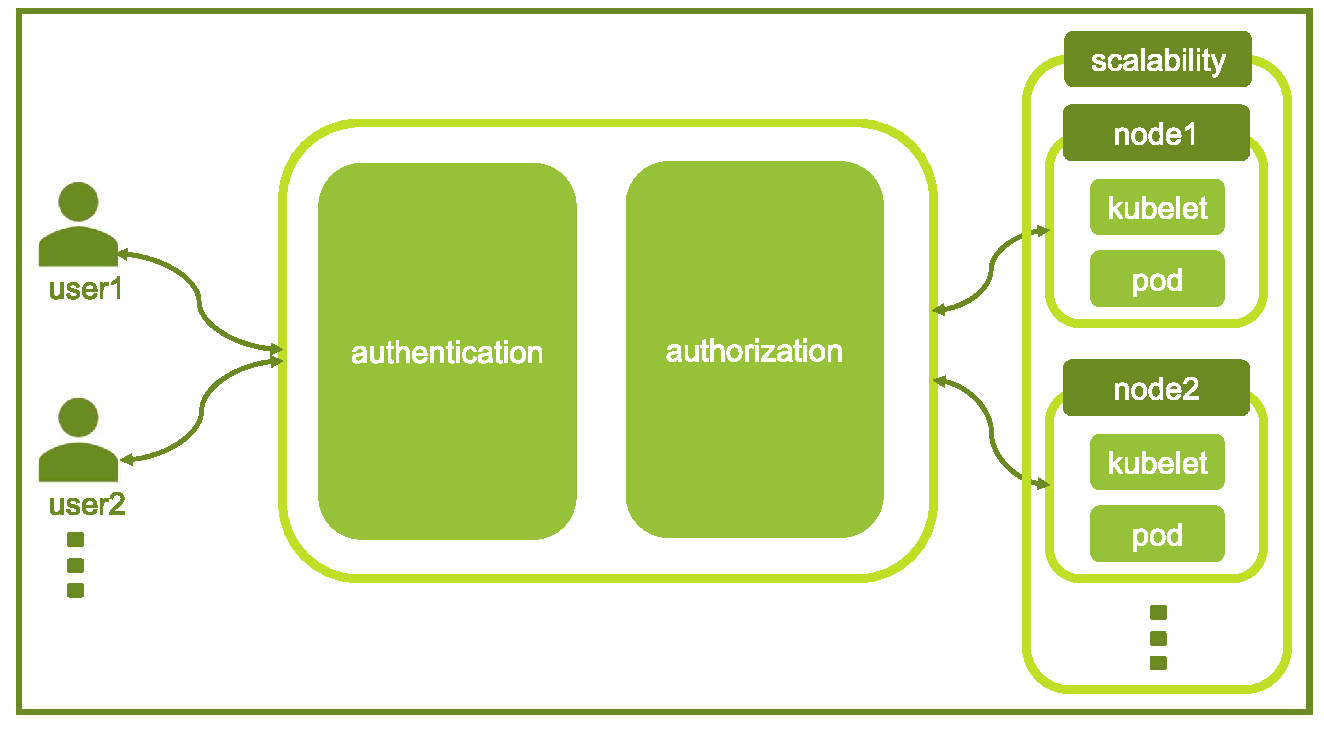
\includegraphics[width=16.88cm,height=9cm]{Thesis/Figures/title.pdf}
\end{textblock*}

\begin{textblock*}{13cm}[0,0](3.45cm, 2.9cm + 9cm + 9.2cm)
\singlespacing
\begin{table}[h!]
	\begin{tabular}{p{3.5cm}p{7cm}R{4.2cm}}
		Author: 	&	Muhammad Fahad Ali, 22995110\\
		& & \\
		Supervisor(s):		&	Prof. Dr.-Ing. Jörg Franke
            & &
                              &  Benedikt Scheffler, M.Sc.	& \\ 
		& & \\
                                    
		Submission date: 	&	30.10.2024 				& \\
		Processing time:	&	\BEARBEITUNGSZEIT\ months &
	\end{tabular}
\end{table}
\end{textblock*}

%\topmargin2cm
%\thispagestyle{empty}
%\renewcommand{\baselinestretch}{1.25}\normalsize
\mbox{ }

\newpage
\thispagestyle{empty}



			    % Deckblatt

	\chapter*{Declaration}
\thispagestyle{empty}
I hereby declare that I have written this thesis without outside help and without using any sources other than those indicated. This thesis has not been submitted in the same or a similar version to any other examination office and been accepted as part of an examination performance. All statements that have been adopted literally or paraphrased are marked as such.\\
\vspace{1.5cm}

Nürnberg, 30.09.2024\\[-5mm]
\hspace*{10.4cm}\rule[-0.3pt]{0.35\linewidth}{0.4pt}\\[0mm]
\hspace*{11.5cm}Muhammad Fahad Ali

%\newpage
\thispagestyle{empty}
\mbox{ }
\newpage			% Erklaerung, dass alles alleine gemacht wurde
        
	\frontmatter				% Roemische Seitennummerierung

	%\nopagebreak
	\cleardoublepage
	\currentpdfbookmark{Contents}{Contents}	% Lesezeichen fuer Inhaltsverzeichnis
	\tableofcontents			% Inhaltsverzeichnis
	
	

% Inhaltsverzeichnislayout
\setcounter{tocdepth}{3} % 3 Gliederungsebenen im Inhaltsverzeichnis

% Formatierung der Verzeichnisse im Inhaltsverzeichnis
\titlecontents{chapter}
[0em]	% Abstand linker Textrand bis Kapitelueberschriften
{}	% Textformatierung
{}	% Abstand und Nummerierung vor Kapitelueberschriften
{}
{\vzPunkte\contentspage} % Formatierung nach Titel bis zur Seitenzahl


% Define new list for code snippets
\newlistof{listingsnippets}{lol}{List of Code Snippets}


% Define how code snippets should appear in the list
\newcommand{\listingsnippet}[2]{
  \refstepcounter{listingsnippets} 
  \addcontentsline{lol}{listingsnippets}{\protect\numberline{\thelistingsnippets}#1}%
  \begin{tcolorbox}[colback=white, colframe=black, 
    boxrule=0.5mm, sharp corners=south, 
    bottomrule=0.5mm, toprule=0.5mm, left=0mm, right=0mm, coltitle=black]
    \begin{lstlisting}
#2
    \end{lstlisting}
  \end{tcolorbox}
  \vspace{-0.5\baselineskip}
  \begin{center} % Center the caption
    \textit{Code Snippet \thelistingsnippets: #1} 
  \end{center}
  \label{listingsnippet:\thelistingsnippets}
}



% Custom format for list of code snippets (optional)
\renewcommand{\cftlistingsnippetsleader}{\cftdotfill{\cftdotsep}} % Dotted lines in list


% Abbildungsverzeichnis
\cleardoublepage
\addtocontents{lof}{\vskip -0.35cm}
\renewcommand{\cftfigleader}{\vzPunkte}
\renewcommand{\cftfigindent}{0em}
\listoffigures%


% Tabellenverzeichnis
\cleardoublepage
\addtocontents{lot}{\vskip -0.35cm}
\renewcommand{\cfttableader}{\vzPunkte}
\renewcommand{\cfttabindent}{0em}
\listoftables%


\cleardoublepage
\listoflistingsnippets % Generates the list of code snippets
\addcontentsline{toc}{chapter}{List of Code Snippets} % Add the generated list to TOC

% Abkuerzungs- und Symbolverzeichnis
\cleardoublepage
\printnomenclature			% Abkürzungs- und Symbolverzeichnis


% Formatierung des Inhaltsverzeichnisses
\titlecontents{chapter}
[1em]	% Abstand linker Textrand bis Kapitelueberschriften
{\vspace{12pt}\bf}	% Textformatierung
{\contentslabel{1em}}	% Abstand und Nummerierung vor Kapitelueberschriften
{}
{\vzPunkte\contentspage\vspace{8pt}} % Formatierung nach Titel bis zur Seitenzahl

\titlecontents{section}
[2.79em] % Abstand linker Textrand bis Kapitelueberschriften
{} % Textformatierung
{\contentslabel{1.809em}} % Abstand und Nummerierung vor Kapitelueberschriften
{}
{\vzPunkte\contentspage} % Formatierung nach Titel bis zur Seitenzahl

\titlecontents{subsection}
[5.387em] % Abstand linker Textrand bis Kapitelueberschriften
{} % Textformatierung
{\contentslabel{3em}}% Abstand und Nummerierung vor Kapitelueberschriften
{}
{\vzPunkte\contentspage} % Formatierung nach Titel bis zur Seitenzahl

% Optional: Renaming Bibliography
%\renewcommand\bibname{References}


	\mainmatter				    % Arabische Seitennummerierung

	%%%%%%%%%%%%%%%%%%%%%%%%%%%%%%%%%%%%%%%%%%%%%%%%%%%%%%%%%%%%%%%%%%%%%%%%%%%%%%%%%%%%%%%%%%%%%%
	%%%%   FILL WITH OWN CONTENT                                                               %%%
	%%%%%%%%%%%%%%%%%%%%%%%%%%%%%%%%%%%%%%%%%%%%%%%%%%%%%%%%%%%%%%%%%%%%%%%%%%%%%%%%%%%%%%%%%%%%%%

%
%	The insertion of chapters is done here:
%

		\chapter[Introduction]{Introduction}
....


  
		
\chapter{State of the Art}

The basic ideas of cloud-native architecture and best practices for achieving a secure, scalable and distributed architecture for AI models are explained in detail in this chapter. A solid understanding of these underlying concepts is required to fully comprehend the approaches identified and explored in the literature review.

\section{Cloud-Native Architectures}

Cloud-native technologies have transformed the landscape of application development, deployment and management by leveraging cloud environments to their fullest potential \cite{r9}. These technologies focus on creating applications as a collection independently deployable services which are loosely coupled, allowing the integration of modules within a cloud-native infrastructure \cite{r10}. Key principles of this approach include containerization, microservices architecture, declarative APIs, continuous integration and delivery \abk{CI/CD}{Continuous Integration and Delivery} and infrastructure as code \abk{IAS}{Infrastructure as Code} \cite{r11}. By embracing cloud-native methodologies, organizations can achieve greater scalability, agility and resilience, enabling the delivery of innovative and dependable software solutions \cite{r12}. In modern software development, scalability and resilience are paramount due to the heightened demand for applications that are both highly available and responsive \cite{r13}. Scalability is the capability of a system to manage varying workloads effectively, accommodating sudden traffic spikes or a steady increase in users \cite{r14}. Resilience ensures that applications continue to function despite failures or disruptions in the underlying infrastructure \cite{r15}. To meet user expectations and ensure business continuity while competing in digital economy, scalability and resilience qualities must be achieved.



\section{Scope and Relevance}

Although this thesis report deals with the principles of secure, scalable and distributed computing, in particular the topic of authentication and authorization using the principles of RBAC and SSO. It also looks at the Ray framework for scalability in distributed computing. Ray is particularly effective in this area because, in addition to the ease of use of the \abk{API}{Application Programming Interface}, it provides easy scalability, effective and resilient fault tolerance and high performance. All of these features make Ray a worthy tool for developers and organizations that want to build highly efficient and reliable distributed applications. Thus, when considering the questions of secure and scalable distributed computation, it is paramount to achieve proper authentication and authorization. Computer security is in a state of flux constantly, with examples of effective solutions include RBAC as well as SSO, both of which help in the protection of resources as well as ease the management of user details. RBAC in Kubernetes, involves the use of RoleBinding and ClusterRoleBinding resources to enable efficient management of access control by namespace and cluster \cite{burns2022Kubernetes}. SSO improves the user experience and security since the user only has to provide the credentials once and the system provides access rights to multiple applications and services which helps to streamline the access control and ensure that the administrative overhead is also reduced \cite{jangda2020sso}. Through embedding the identified Ray framework in combination with such sound RBAC and SSO solutions, it is possible to provide organizations with the secure, large-scale and efficient distributed computation environments. \cite{zaharia2012resilient, moritz}


\section{Fundamentals of Cloud-Native Architecture}

Cloud-native technologies consist a set of methodologies, practices and tools designed for cloud environments. These include containerization and microservice architectures, which allows to achieve scalability, agility and resilience in cloud platforms to deliver cutting-edge and well grounded software solutions. \cite{r16}

\subsection{Containerization}

Containerization is a technique that packages an application with all its necessary dependencies into a lightweight, single unit called container. This approach guarantees consistent performance across different computing environments by encapsulating all components required to execute the application, such as libraries, dependencies and configuration files within the container. Unlike virtual machines, containers share the host system kernel, making them more efficient in terms of resource utilization and startup time. Docker is one of the most widely used containerisation platforms, providing tools for creating, managing and deploying containers, enabling developers to build, test and deploy applications with ease and consistency. The containers architecture, including their interaction with the host system, can be visualized in \autoref{fig:Container Architecture}. \cite{Docker_container}

\captionsetup{justification=centering}
\begin{figure}[h]
\centering
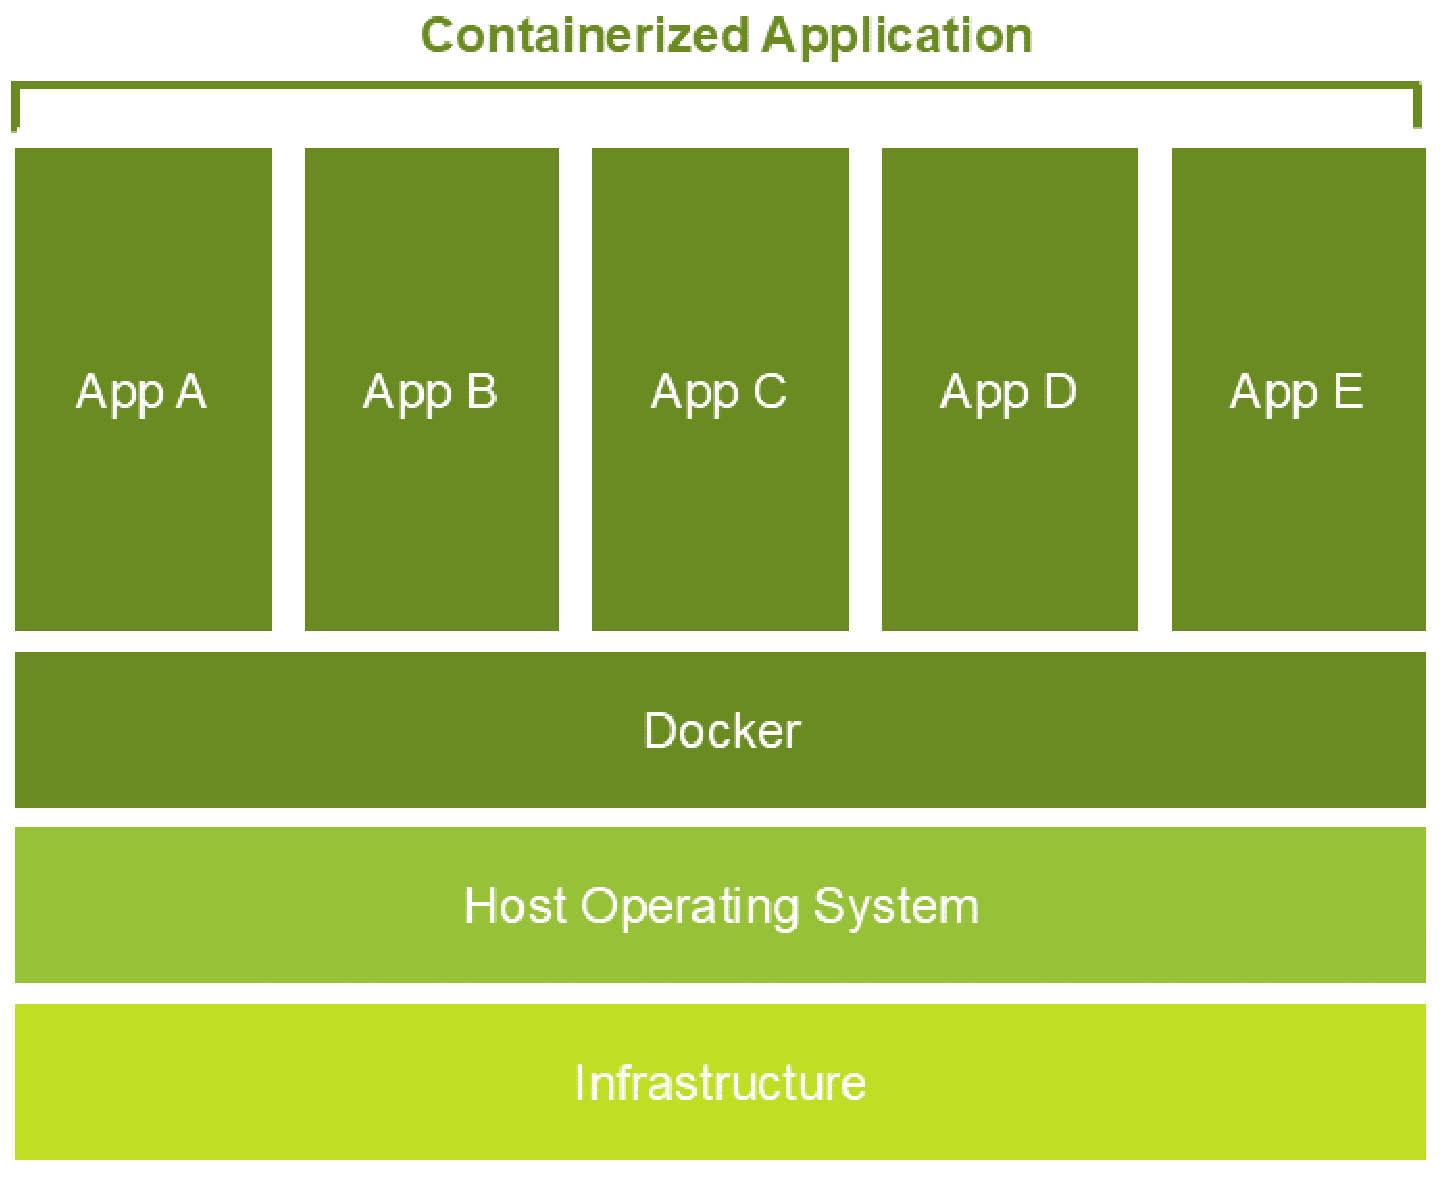
\includegraphics[width=0.8 \linewidth]{Thesis/Figures/Slide3.pdf}
\caption{\label{fig:Container Architecture}Container Architecture \cite{Docker_container}}
\end{figure}

\vspace{0.2cm}

The architecture of containers allows for significant improvements in development workflows and operational efficiency \cite{Kubernetes_doc}. By isolating applications and their dependencies from the host system, containers eliminate the common problem of \texttt{dependency hell} and environment inconsistencies \cite{Kubernetes_doc}. This isolation also enhances security by limiting the applications access to the host system \cite{Kubernetes_doc}. Additionally, container orchestration tools like Kubernetes have emerged to manage the deployment, scaling and operation of containerized applications across clusters of machines, further enhancing the robustness and scalability of containerized solutions \cite{Kubernetes_doc}. Overall, containerization has revolutionized the way applications are developed, deployed and managed, making it a cornerstone technology in modern DevOps practices \cite{redhat_docs}.

\textbf{Docker}

Docker is an open source platform that simplifies the development, deployment and distribution of applications. It packages applications and their necessary dependencies into standardised units called containers. These containers run in isolation on top of the operating system kernel, providing a lightweight and efficient environment for running code. Docker enables developers to easily create, manage and deploy containers, allowing applications to run anywhere without modification and ensuring seamless portability across environments. In addition, Docker integrates with third party tools to improve the deployment and management of containers, particularly in cloud-native environments. Docker works on a client server model, where the Docker client sends requests to the Docker server, which handles those requests. The platform consists of several key components including the Docker client, Docker server, Docker images, Docker registries and Docker containers. Docker images are created using read-only templates, with a base image such as Ubuntu serving as the foundation. Images can either be created from scratch or modified. Docker files provide an automated method of building images by following a set of instructions. These images are stored in Docker registries, such as Docker Hub, which can be public or private. Finally, Docker containers are created from Docker images and encapsulate everything needed to run an application in an isolated environment. This isolation ensures consistency and reliability across different platforms, making Docker a powerful tool for modern software development. \cite{rad2017introduction}

\subsection{Microservices Architecture}

Microservices architecture is an approach where applications are divided into small, independently deployable services, each responsible for handling different business functions, as shown in \autoref{fig:Microservice Architecture}. These services interact with each other using well-defined APIs and communication protocols, allowing developers to focus on individual components separately. This approach promotes scalability, flexibility and modularity by allowing teams to develop and scale services independently, resulting in faster development cycles and improved fault isolation. \cite{r22}

\clearpage

\captionsetup{justification=centering}
\begin{figure}[h]
\centering
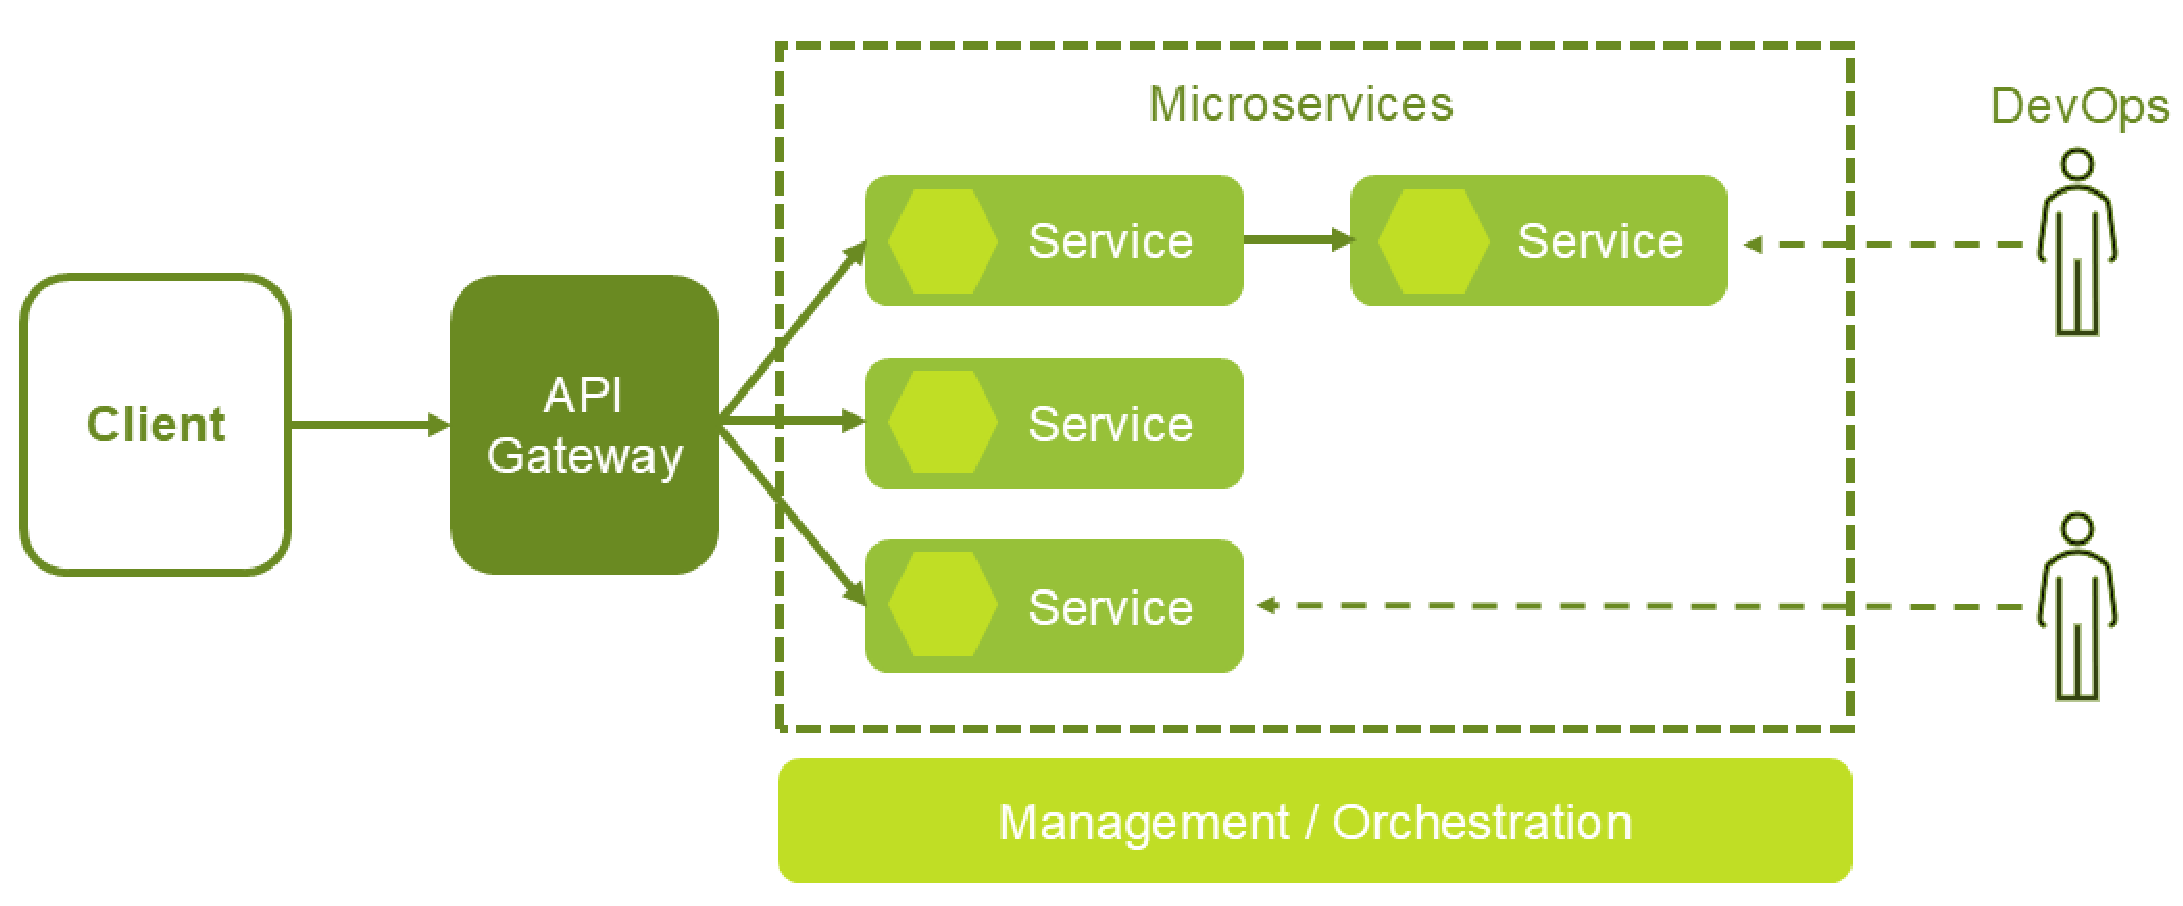
\includegraphics[width=0.9 \linewidth]{Thesis/Figures/Slide4.pdf}
\caption{\label{fig:Microservice Architecture}Microservice Architecture \cite{r23}}
\end{figure}


\subsection{Container Orchestration}

Container orchestration remains essential for scalable and automated coordination of microservice architectures, managing the lifecycle of containers and services in a compute cluster. Typically, end users submit their jobs to a cluster manager, one of the core components of the orchestration system. The cluster manager is responsible for assigning tasks to worker nodes within the cluster. These clusters, composed of either physical or virtual machines, execute the required tasks. An application or job often relies on multiple services, each running in containers with diverse tasks. Container orchestrators provide an abstraction layer that simplifies the management of complex environments and architectural solutions, whether for client facing infrastructures or cloud services. Popular on premise orchestrators include Kubernetes, Borg and Mesos, typically installed and configured as standalone software. In the cloud, Google Kubernetes engine \abk{GKE}{Google Kubernetes Engine}, Microsoft Azure Kubernetes service \abk{AKS}{Azure Kubernetes Service} and Amazon elastic Kubernetes service \abk{EKS}{Elastic Kubernetes Service} are widely used hosted solutions with predefined, easily configurable setups. \cite{carrion2022Kubernetes}

Another core component of the container orchestrators is the scheduling module, which embodies the component in question and aimed towards finding which node should execute an incoming task considering various factors which include availability of resources, necessary node affinities, or location of the data to be processed. Furthermore, there is also the rescheduler component that assists in transforming tasks location to group loads or optimise the usage of resource. Others consist of the resource allotment module through which resources of the cluster are assigned either dynamically or even statically and the load distribution module which enforces the distribution of the submitted tasks in line with some specified criteria within the cluster. The autoscaling module where resources are adjusted either horizontally or vertically based on the workload within the cluster. Also, the admission control module tries to guarantee that the resources requested fit within the cluster’s capacity, whereas the accounting and monitoring modules provide information regarding resource utilization and node health, respectively, for system dependability and fault tolerance purposes as shown in \autoref{fig:Container Orchestration}. These components in total deliver a strong environment for optimal and distributed container processes. \cite{carrion2022Kubernetes}


\captionsetup{justification=centering}
\begin{figure}[h]
\centering
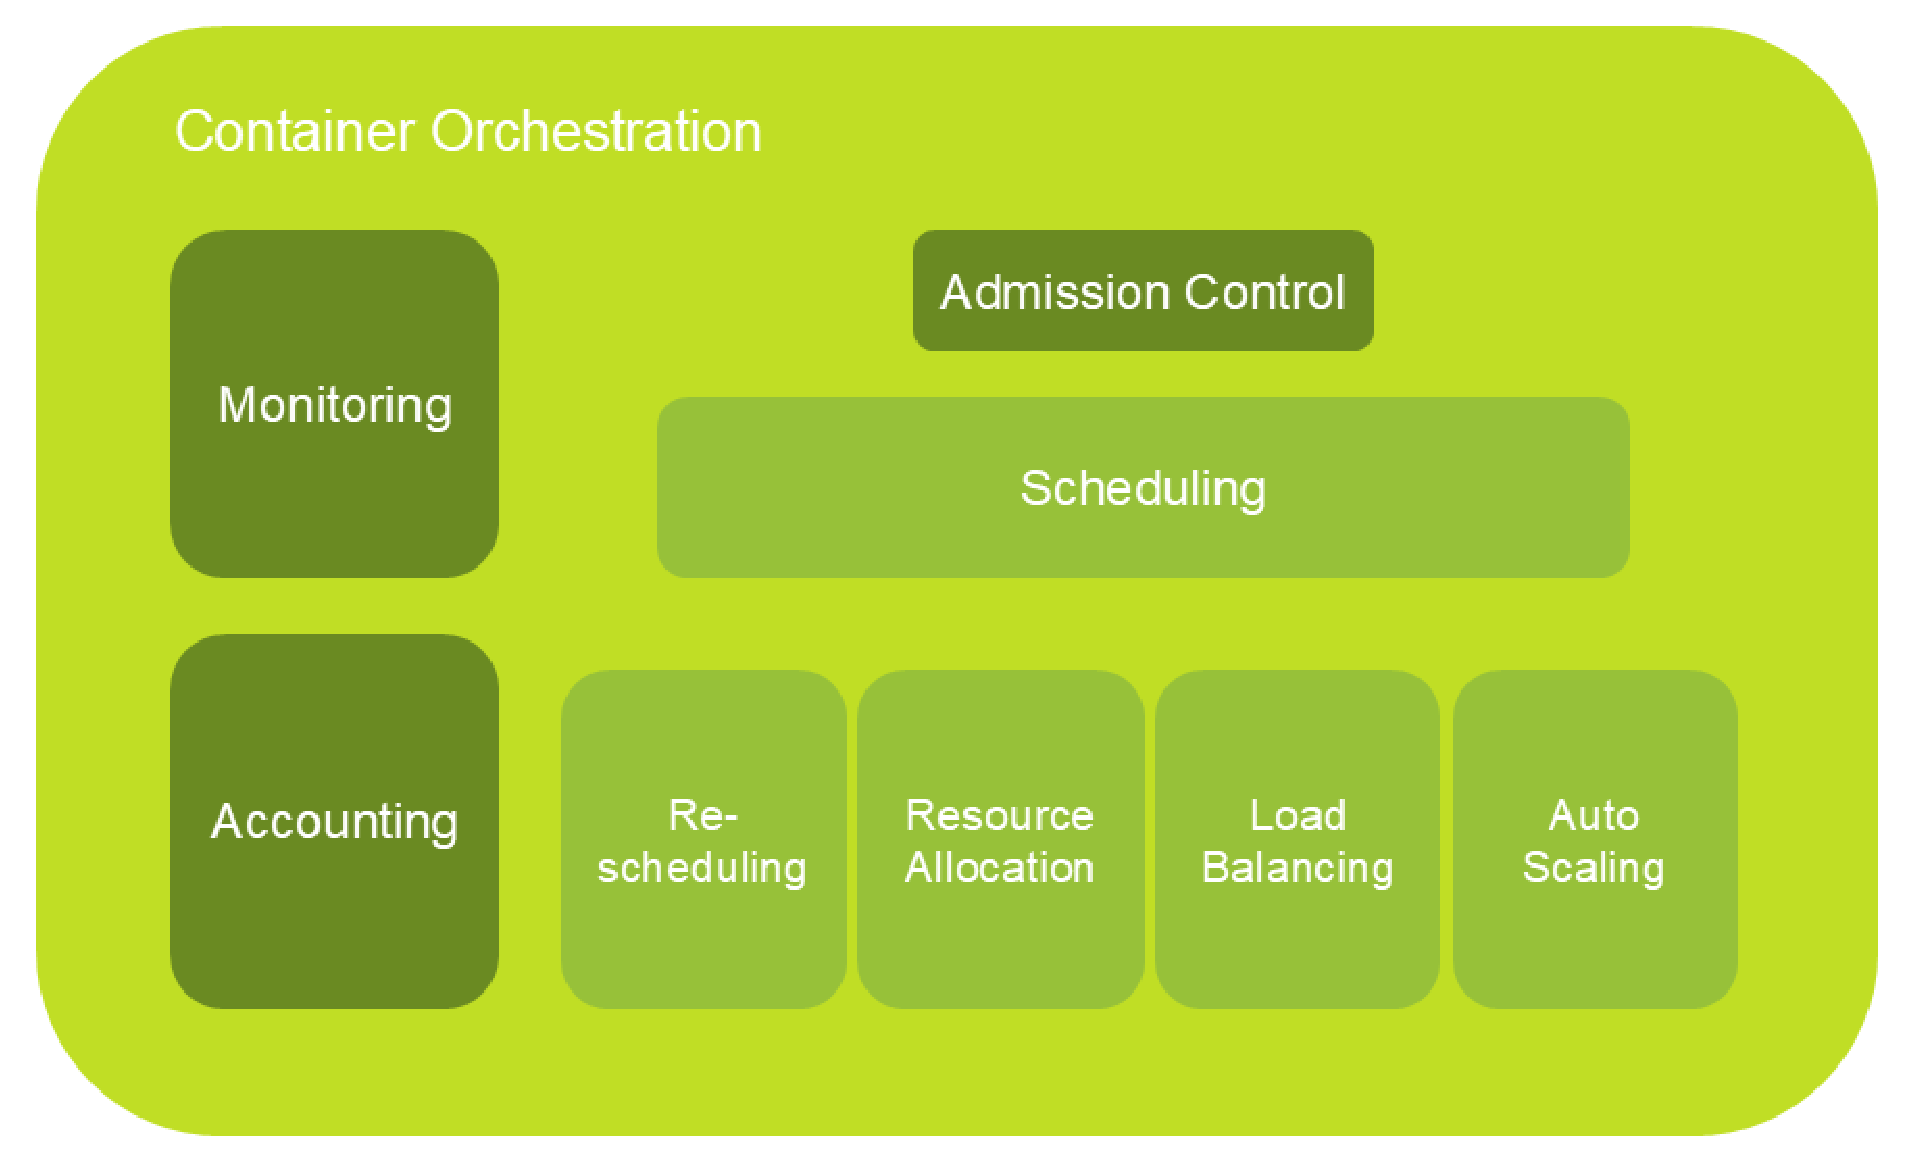
\includegraphics[width=0.8 \linewidth]{Thesis/Figures/Slide34.pdf}
\caption{\label{fig:Container Orchestration}Container Orchestration \cite{carrion2022Kubernetes}}
\end{figure}


\section{Best Practices for Designing Scalable Cloud-Native Architectures}

By integrating technologies like distributed tracing, chaos engineering and circuit breaking, cloud-native architectures can achieve high levels of scalability, flexibility and reliability. These practices allows organizations to fully leverage the advantages of cloud computing, ensuring their applications are resilient and capable of handling diverse and unpredictable workloads. \cite{r16}

\subsection{Distributed Tracing}

Distributed tracing is essential to understand how the requests flow through complex distributed systems \cite{r24}. It allows developers to track each requests as they passed through multiple microservices, facilitating the diagnosis of performance issues, pinpointing bottlenecks and enhancing application performance \cite{r25}. As shown in \autoref{fig:Distributed Tracing}, a service with a unique ID initiates a transaction by calling microservices A through E. Microservice A starts by invoking microservice B, which in turn calls microservices C and D, while A also calls microservice E, all of which are visualized as time spans to represent the complete trace of the request \cite{logz2024tracing}.

\clearpage

\captionsetup{justification=centering}
\begin{figure}[h]
\centering
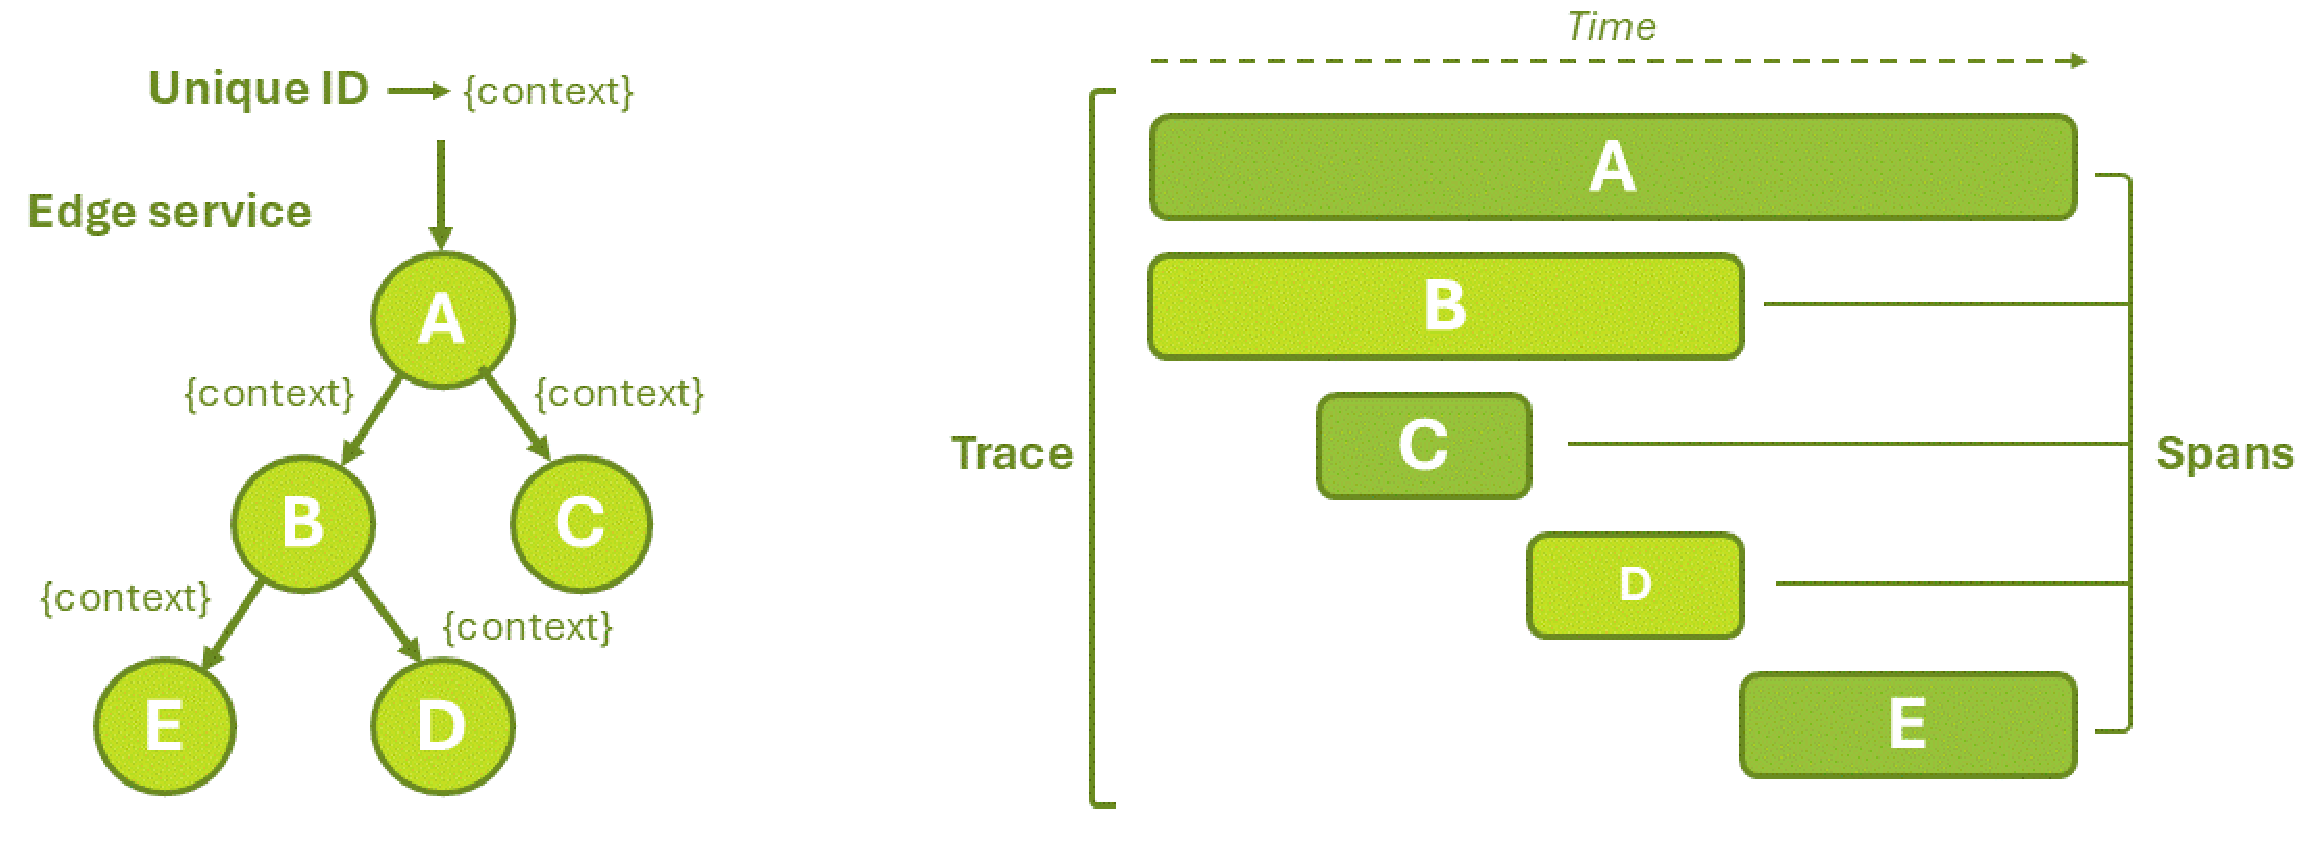
\includegraphics[width=1 \linewidth]{Thesis/Figures/Slide33.pdf}
\caption{\label{fig:Distributed Tracing}Distributed Tracing \cite{logz2024tracing}}
\end{figure}


\subsection{Circuit Breaking}


Circuit breaking is a technique that uses interceptors to check the health of services in terms of availability and responsiveness.The circuit breaker automatically rejects requests when a microservice is down, as shown in \autoref{fig:Circuit Breaker}. This prevents applications from waiting for a timeout due to service unavailability. This approach reduces application response time by eliminating unnecessary retries. When the service becomes available again, the circuit breaker automatically resets, allowing requests to pass through. To implement circuit breakers, all microservices must update and call each other using circuit breaker proxies. In addition, choosing appropriate timeout values for the circuit breaker can be challenging. Despite these trade-offs, circuit breakers are essential for maintaining and improving system responsiveness. \cite{r28}.


\captionsetup{justification=centering}
\begin{figure}[h]
\centering
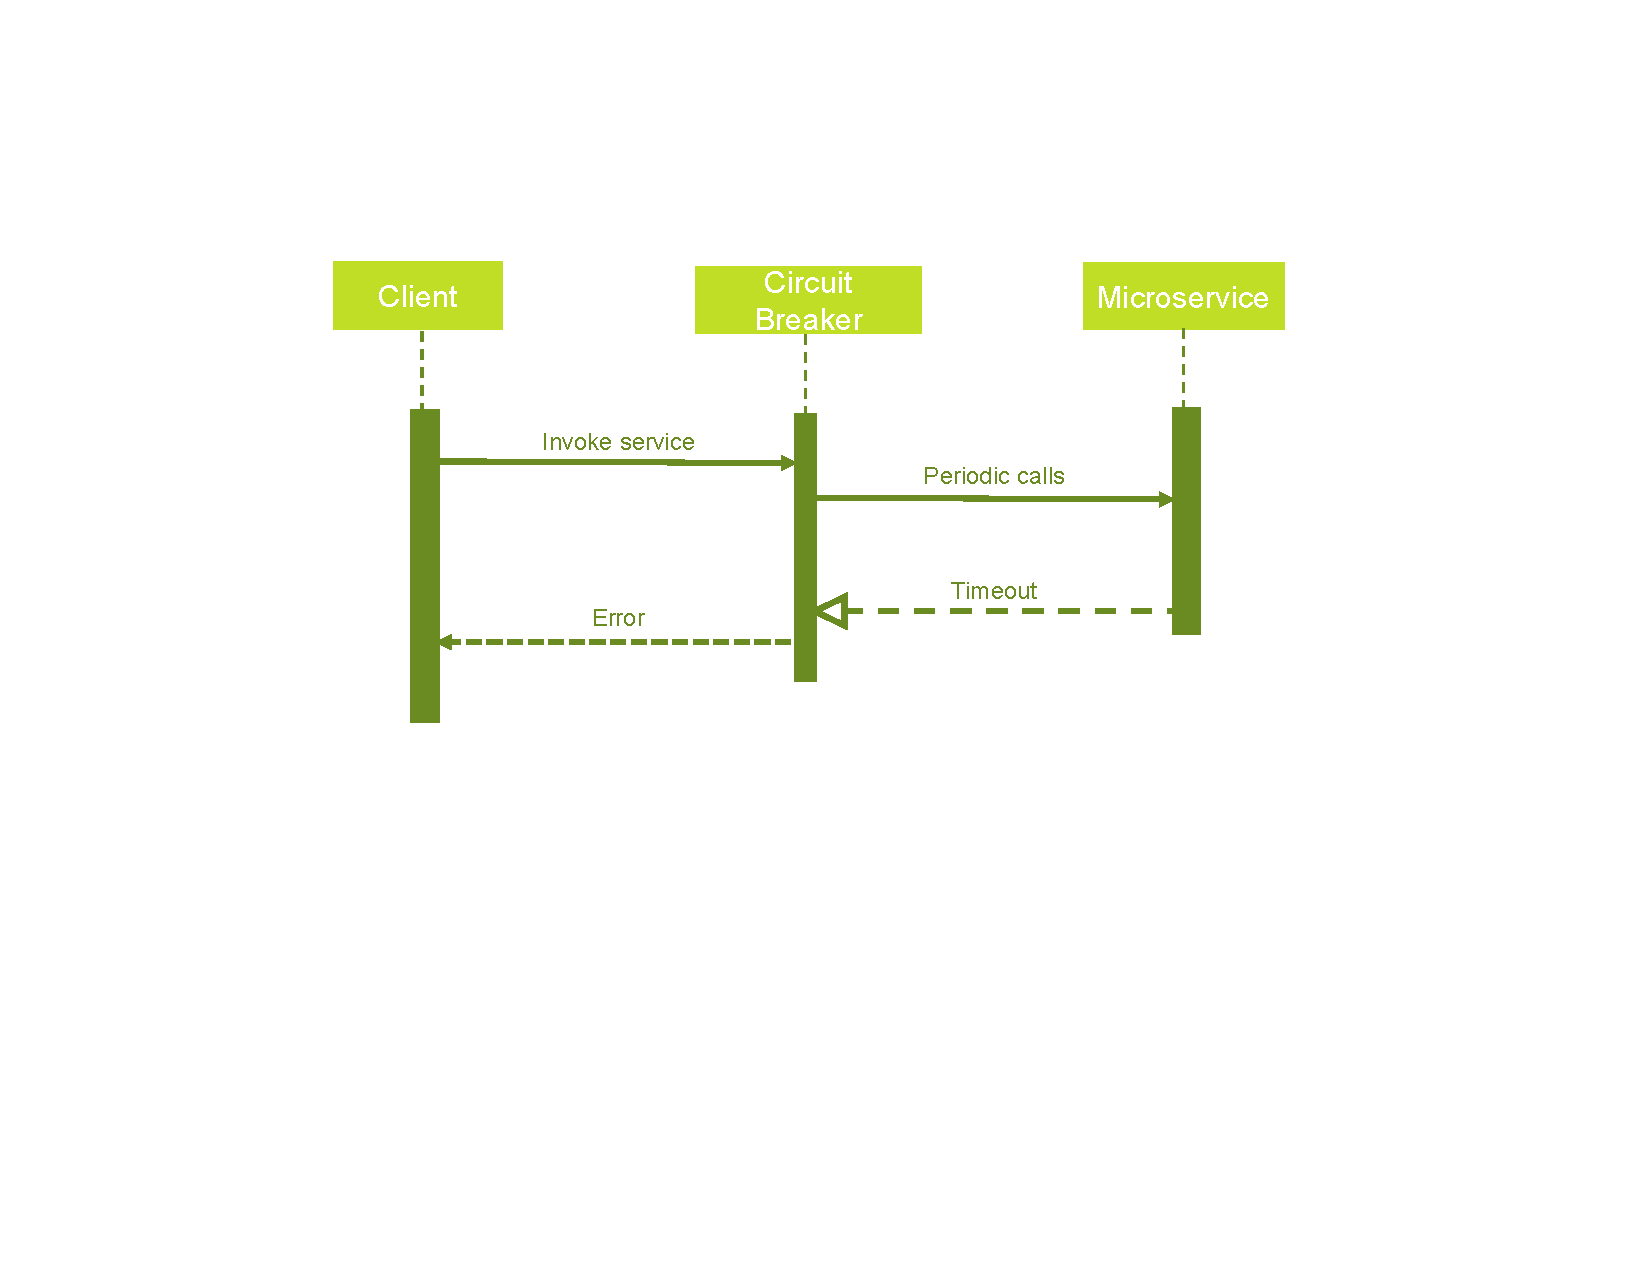
\includegraphics[width=1 \linewidth]{Thesis/Figures/Slide32.pdf}
\caption{\label{fig:Circuit Breaker}Circuit Breaker \cite{goyal2019circuit}}
\end{figure}


\subsection{Chaos Engineering}

The aim of chaos engineering is to test the resilience of distributed systems to determine how resilient they are. It involves simulation-based fault injection and is defined as "The discipline of experimenting on a distributed system to build confidence in the system's ability to withstand turbulent conditions in production". The basic idea behind chaos engineering is to deliberately subject the system to adverse conditions modelled on those that may occur in a real production environment. This method helps to identify any defects and provides insight into the resilience of the system. Organisations can proactively avoid such problems by identifying these vulnerabilities before they result in user problems. \cite{r29}

\section{Key Components of Cloud-Native Ecosystems}

This section examines the essential elements of cloud-native ecosystems, focusing on Kubernetes for container orchestration and resource autoscaling, as well as the tools and technologies required to secure and scale cloud-native architectures.

\subsection{Kubernetes}

Kubernetes is an open source container orchestration platform that automates the deployment, scaling and management of containerised applications. It provides a robust set of features, including a key-value pair store, API server, controller manager and scheduler, that streamline container operations and abstract the complexity of the underlying infrastructure, as shown in \autoref{fig:Kubernetes Architecture}. This abstraction allows developers to focus on building and deploying applications without worrying about the internal infrastructure. \cite{r32}

\captionsetup{justification=centering}
\begin{figure}[h]
\centering
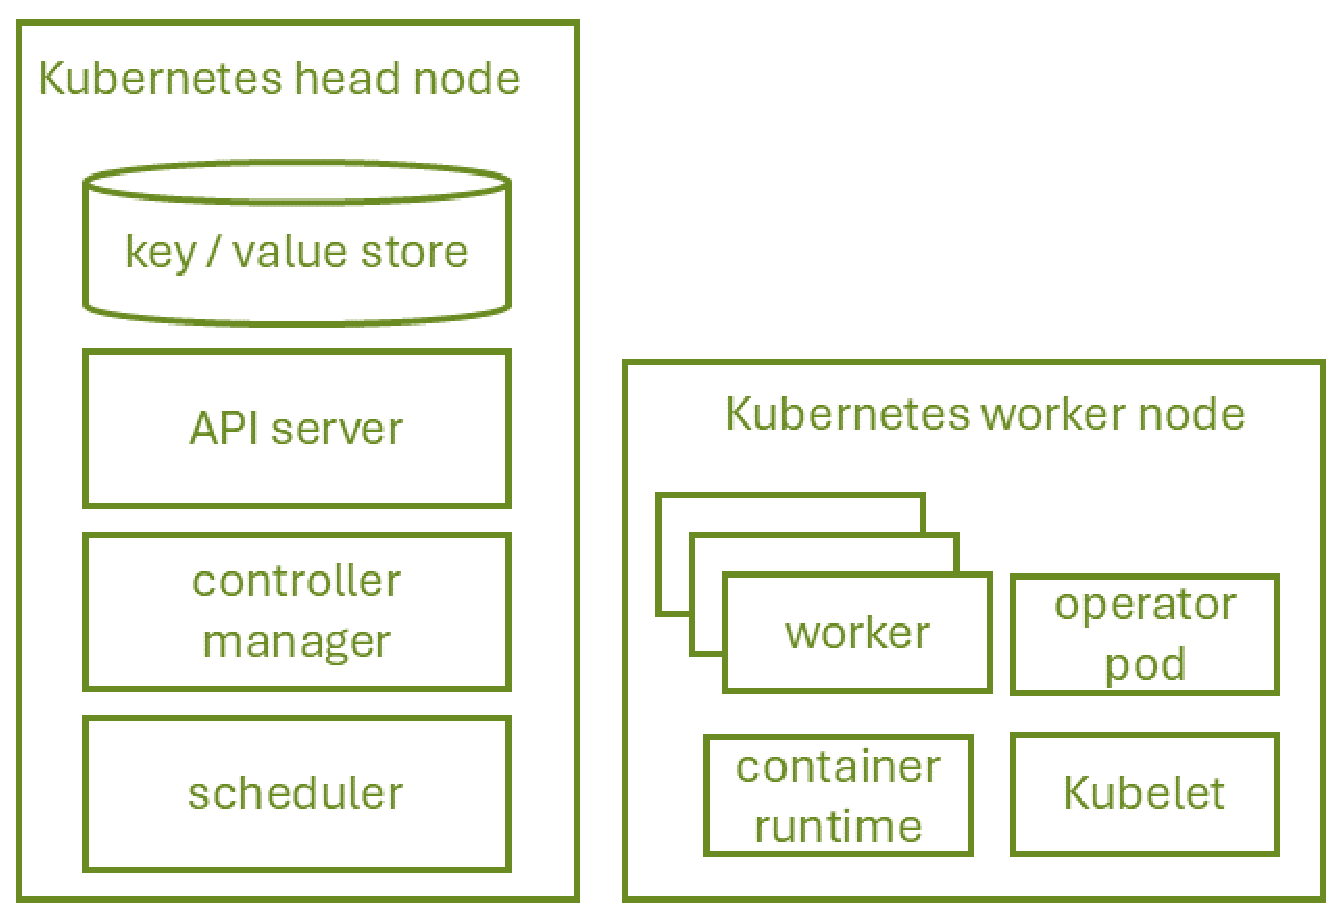
\includegraphics[width=0.8 \linewidth]{Thesis/Figures/Slide16.pdf}
\caption{\label{fig:Kubernetes Architecture}Kubernetes Architecture \cite{r34}}
\end{figure}

Kubernetes has become the de facto container management platform. It defines a declarative model for specifying a desired system state and implements controller logic that constantly strives to reconcile the actual system state with the desired state. The Kubernetes API server serves REST operations and provides the frontend to the clusters shared state. This state is stored in a key-value store. The values of these keys represent artifacts managed by Kubernetes, such as pods. Pods, which abstract containers, are the smallest deployable units in Kubernetes. Kubernetes manages the lifecycle of pods through various controllers, with the controller manager overseeing numerous controllers, such as the deployment and replica set controllers. For instance, the deployment controller continuously monitors the deployment manifest, which defines how replicated pods should be managed and ensures that the number of running pods matches the desired count in the cluster. \cite{r34}




\textbf{Minikube}


Minikube is a tool that allows developers to run Kubernetes clusters locally, providing a lightweight and easy to use solution for testing and developing Kubernetes applications. It creates a single node Kubernetes cluster within a virtual machine \abk{VM}{Virtual Machine} on a local system, providing an environment that closely simulates a Kubernetes cluster in production. This allows developers to experiment and test Kubernetes applications without having to deploy them to a full scale cloud-based cluster. To get started with Minikube, a few installation steps are required. First, it is necessary to install a hypervisor, which Minikube will use to create the VM. Next, kubectl the command-line tool for managing and interacting with Kubernetes clusters. After that, download and install the Minikube binary specific to the operating system, which simplifies the setup process by providing a single executable. Once everything is installed, you can start the Minikube cluster using the \texttt{minikube start} command. This command starts a local Kubernetes cluster, with Minikube automatically taking care of creating the VM, installing the Kubernetes components and configuring kubectl for use with the local cluster. \cite{sayfan2019hands}

\textbf{Kubectl}


Kubectl is a command-line tool used to interact with the Kubernetes control panel via the Kubernetes API. It allows users to perform various operations on Kubernetes resources. The config file contains kubectl configurations, which are located in the \texttt{\$HOME/.kube} directory, which can also be placed in other locations using the \texttt{KUBECONFIG} environment variable or the \texttt{kubeconfig} flag. The general syntax for using kubectl consists of four elements: command, type, name and flag. The command represents the operation you want to perform, such as creating, retrieving or deleting resources. The resource TYPE refers to the type of Kubernetes resource being managed, such as pod, service or deployment, which can be singular, plural or abbreviated. The NAME is the resource identifier, which is case-sensitive. If the name is omitted, kubectl will retrieve information for all resources of that type. In addition, flags allow you to customise commands by overriding defaults or environment variables. Kubectl also supports operations on multiple resources at once. You can either group resources of the same type, or specify different resource types individually. \cite{Kubernetes_doc}

\clearpage

\textbf{Helm}

Helm is a tool for managing Kubernetes packages, known as charts. A Helm chart is essentially a collection of files and information needed to deploy a Kubernetes application. Helm's purpose is to create charts from scratch, package them into \texttt{.tgz} files and store them in chart repositories or deploy them to Kubernetes clusters. Helm also manages the lifecycle of these charts, which includes installation, upgrades and uninstallation. There are three key components to Helm's structure a chart, a configuration and a release. A chart bundles all the resources needed to create an application, the config contains configuration settings that can be applied to the chart when creating a custom deployment and the release refers to a running instance of the chart combined with a specific configuration. Helm is divided into two primary components the Helm client and the Helm library. The Helm client is serve a command-line interface used by end users for tasks such as local chart development, repository management and release handling. On the other hand, Helm library, handles the core logic for operations like installing, upgrading, or uninstalling charts, while interfacing with the Kubernetes API server to provision resources. \cite{helm_docs}

\textbf{Kind}

Kind (Kubernetes in Docker) is a tool that allows users to create and manage local Kubernetes clusters using Docker containers. It's particularly useful for testing and development, providing a lightweight, easy way to spin up clusters without needing a full cloud-native environment. Kind works by running Kubernetes nodes inside Docker containers, simulating a full Kubernetes cluster. This makes it a preferred choice for local Kubernetes development, as it integrates well with existing Docker environments and simplifies the setup process. One of the key benefits of using Kind is its ability to create multi node clusters with minimal overhead. Developers can easily create clusters to test different Kubernetes features, workflows or applications on their local machines. Kind also inherits Docker's portability, allowing the same Kubernetes environment to be replicated across different machines. It supports most of the core Kubernetes features and can be integrated with continuous integration \abk{CI}{Continuous Integration} pipelines, making it a handy tool for automatically testing Kubernetes deployments during software development processes. However, because it's designed for local use, it lacks some of the scalability and performance optimisations found at the production level in Kubernetes clusters. Kind is a widely adopted solution in the Kubernetes ecosystem, particularly for developers who need a local Kubernetes environment for testing without the complexity of managing an actual Kubernetes infrastructure. \cite{kind_Kubernetes}


\subsection{Kubernetes Autoscaling}

Kubernetes autoscaling is used to control and manage the number of instances running in a cluster based on the load. This capability is necessary for sustaining efficient performance and expenditure in cloud-native applications. Kubernetes supports various types of autoscaling, including horizontal, vertical and cluster level autoscaling. horizontal pod autoscaling \abk{HPA}{Horizontal Pod Autoscaling} is used to increase the number of pods in deployment or replica set while vertical pod autoscaling \abk{VPA}{Vertical Pod Autoscaling} is used to change the container resource requirements. The process of scaling up or down the Kubernetes cluster is done by cluster autoscaler considering the usage of the pods. To achieve autoscaling in Kubernetes, there has to be creation of metrics and specifications of the parameters that should be crossed as the requirements for scaling. For example, the HPA uses metrics that come from the Kubernetes metrics server or any other custom metrics. If the defined metric proves to be higher than a set limit, the HPA will add more pod to help in handling the demand. On the other hand, if the usage goes below the set figure, the status will prescribe the number of pods to decrease. To achieve dynamic scaling, the loads that an application experiences are smoothed out and this makes the application adapt to changing loads on the system without the need for intervention thus increasing resource usage efficiency as well as decreasing the operational costs. \cite{Kubernetes_doc}


\textbf{Horizontal Pod Autoscaler}

HPA is one of the core components of Kubernetes that scales a deployment, a replica set, or a stateful set up or down depending on the observed central processing unit \abk{CPU}{Central Processing Unit} usage or other, user supplied metrics. Specifically, the primary goal of HPA is to make sure that the application can effectively respond to changes in load through the process of scaling out by creating more pods or scaling in by removing the unnecessary pods see \autoref{fig:Horizontal Pod Autoscaling}. HPA operates by constantly making a call to the Kubernetes metrics server to fetch the pods current utilization and then comparing it to the desired or target utilization from the HPA configuration. HPA configuration entails the identification of the target and a value below which a warning message should be generated. For instance, the specific goal of CPU utilization might be set at 70 percent. When the average CPU utilization of all pods in the deployment, HPA will scale up the pods, to spread the load evenly. On the other hand, if the present CPU usage is lesser than this indication, HPA will scale down the amount of pods. This process guarantees the responsiveness of the application in terms of internal and external loads, additionally it ensures efficiency in the use of resources. \cite{Kubernetes_doc}


\captionsetup{justification=centering}
\begin{figure}[h]
\centering
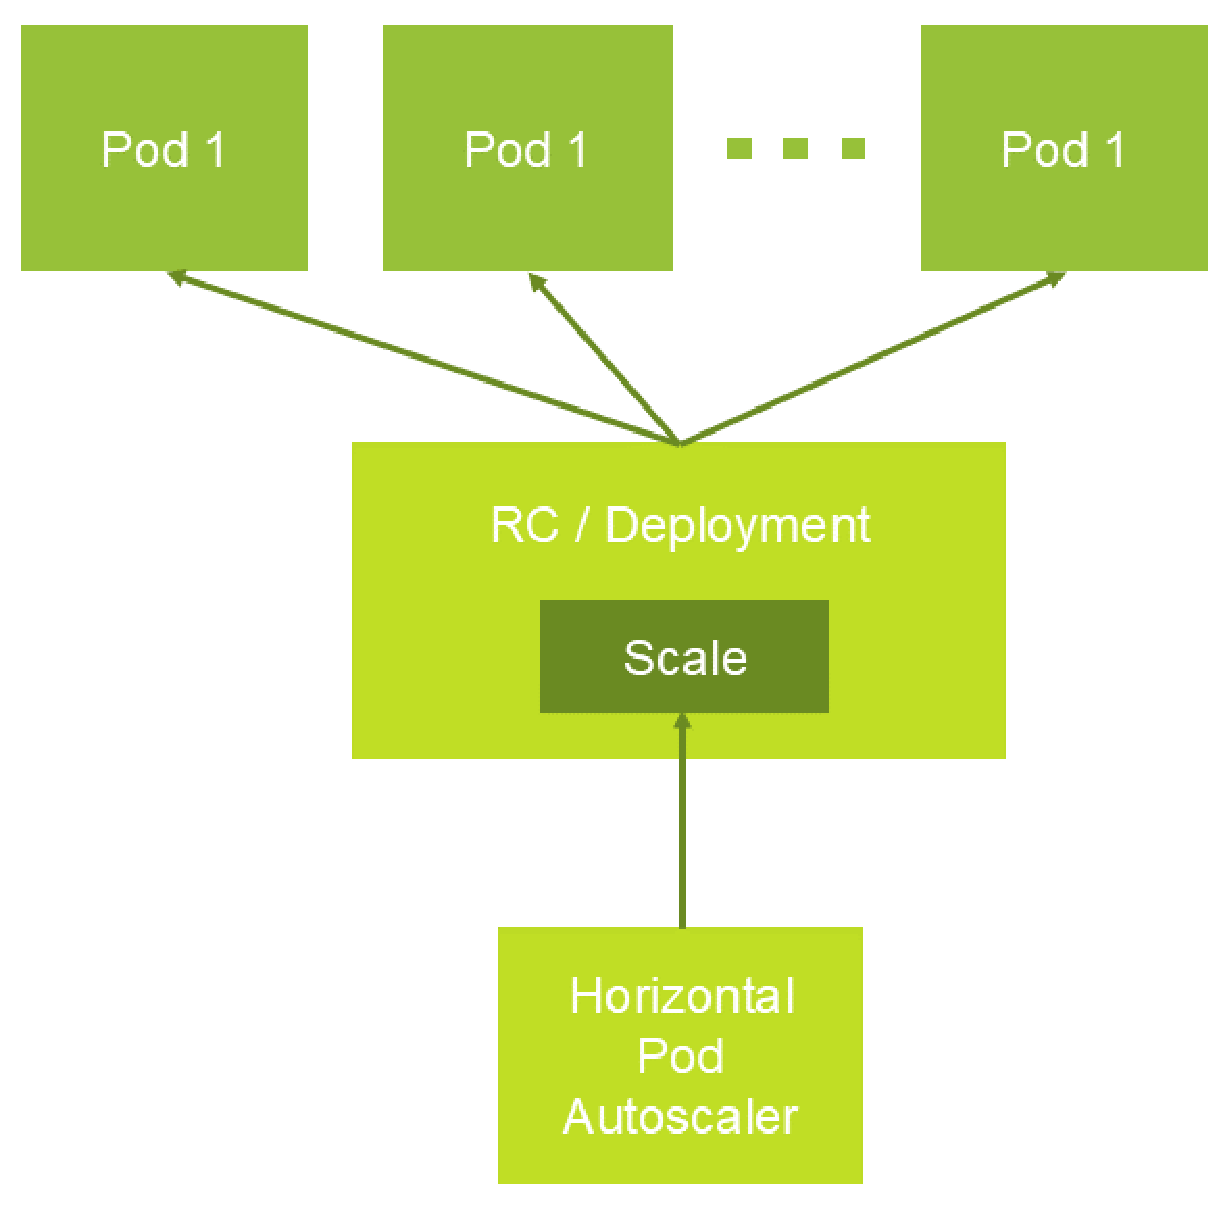
\includegraphics[width=0.6 \linewidth]{Thesis/Figures/Slide35.pdf}
\caption{\label{fig:Horizontal Pod Autoscaling}Horizontal Pod Autoscaling \cite{Kubernetes_doc}}
\end{figure}


\clearpage

\textbf{Vertical Pod Autoscaler}

VPA is another autoscaling feature in Kubernetes that focuses on adjusting the resource requests and limits for containers within a pod, rather than changing the number of pods as shown in \autoref{fig:Vertical Pod Autoscaling}. This autoscaling is very helpful for the applications with fluctuating demand in resources because with this approach the correct amount of CPU and RAM is allocated to each pod. VPA is always checking the resource utilization of pods and may give suggestions on increasing or decreasing the amount of resource provided or even making such changes on its own. \cite{vertical_pod_autoscaler}

\captionsetup{justification=centering}
\begin{figure}[h]
\centering
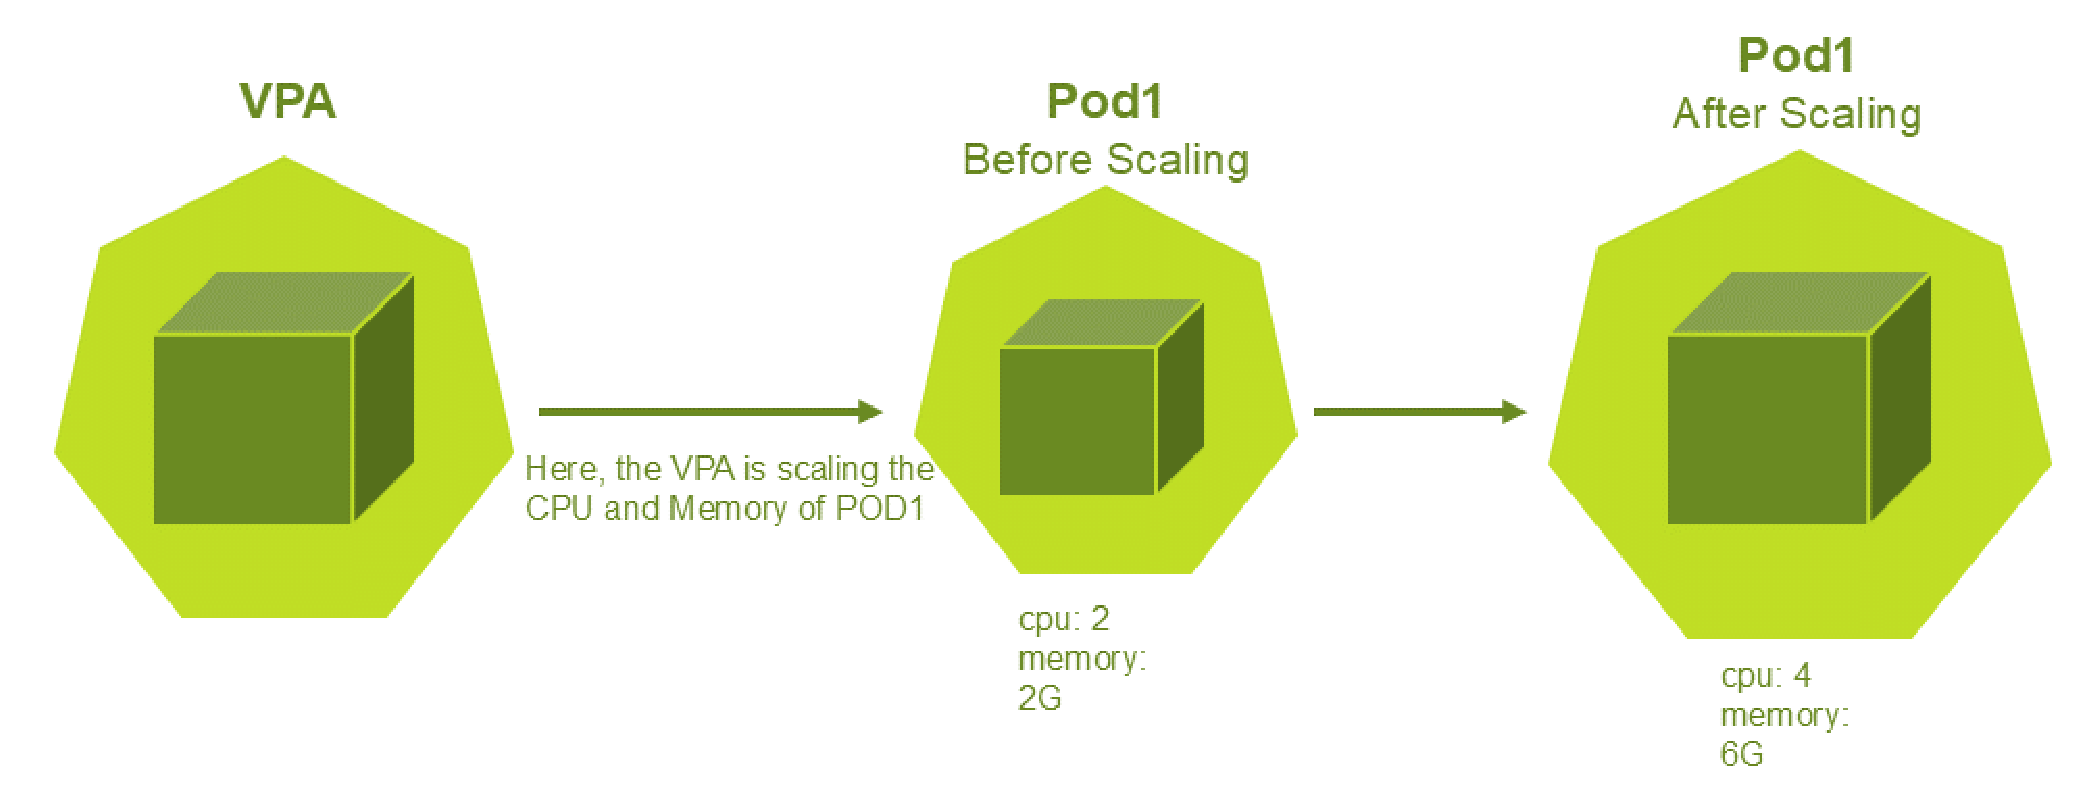
\includegraphics[width=1 \linewidth]{Thesis/Figures/Slide36.pdf}
\caption{\label{fig:Vertical Pod Autoscaling}Vertical Pod Autoscaling \cite{Kubernetes-vpa}}
\end{figure}

The VPA operates in three modes \texttt{Off}, \texttt{Auto} and \texttt{Recreate}. In \texttt{Off} mode, the VPA provides recommendations of changes that need to be made without actually making the changes. In \texttt{Auto} mode, which means that it optimizes them during the pod’s existence. \texttt{Recreate} mode entails restating the pod to make necessary changes on the available resource options. Still, this kind of flexibility is very useful to administrators because they can select a flow that is suitable for their application and the manner in which it will be run. In preventing wastage of resources, VPA assists in avoiding scenarios that may lead to performance throttle by ensuring that the value of pods converge towards the set limit, thus improving the stability of the Kubernetes applications. \cite{vertical_pod_autoscaler}




\section{Authentication and Authorization in Cloud-Native Architectures}

Authentication and authorization are critical to securing applications and services in cloud-native architectures. These architectures leverage the clouds inherent scalability, flexibility and distributed nature, necessitating modern, dynamic approaches to access control. Traditional security measures are often inadequate in such environments, where resources are highly distributed and dynamically scaled \cite{mohamed2024cloud}. Authentication involves verifying the identity of users or services, often implemented through techniques such as multi factor authentication \abk{MFA}{Multi Factor Authentication}, SSO and federated identity providers. SAML OAuth and OIDC are widely used standards that facilitate secure authentication and authorization, ensuring that users identities are verified and managed securely across various applications and services. \cite{r38, r39}

Authorization, on the other hand, determines the actions that authenticated users or services are allowed to perform only within a pod, rather than changing the number of pods as shown in \autoref{fig:Authentication and Authorization}. Cloud-native environments commonly employ RBAC and ABAC to manage permissions efficiently. RBAC assigns permissions to roles, simplifying management by grouping users into roles, based on their job functions, as seen in systems like Kubernetes \cite{r40}. ABAC, however, provides more granular control by using user attributes, resource types and environmental contexts to define access policies, thus allowing for dynamic and context aware access decisions \cite{r41}. Both methods are essential in ensuring that only authorized users can access specific resources, thereby enhancing security and operational efficiency in cloud-native architectures.

\captionsetup{justification=centering}
\begin{figure}[h]
\centering
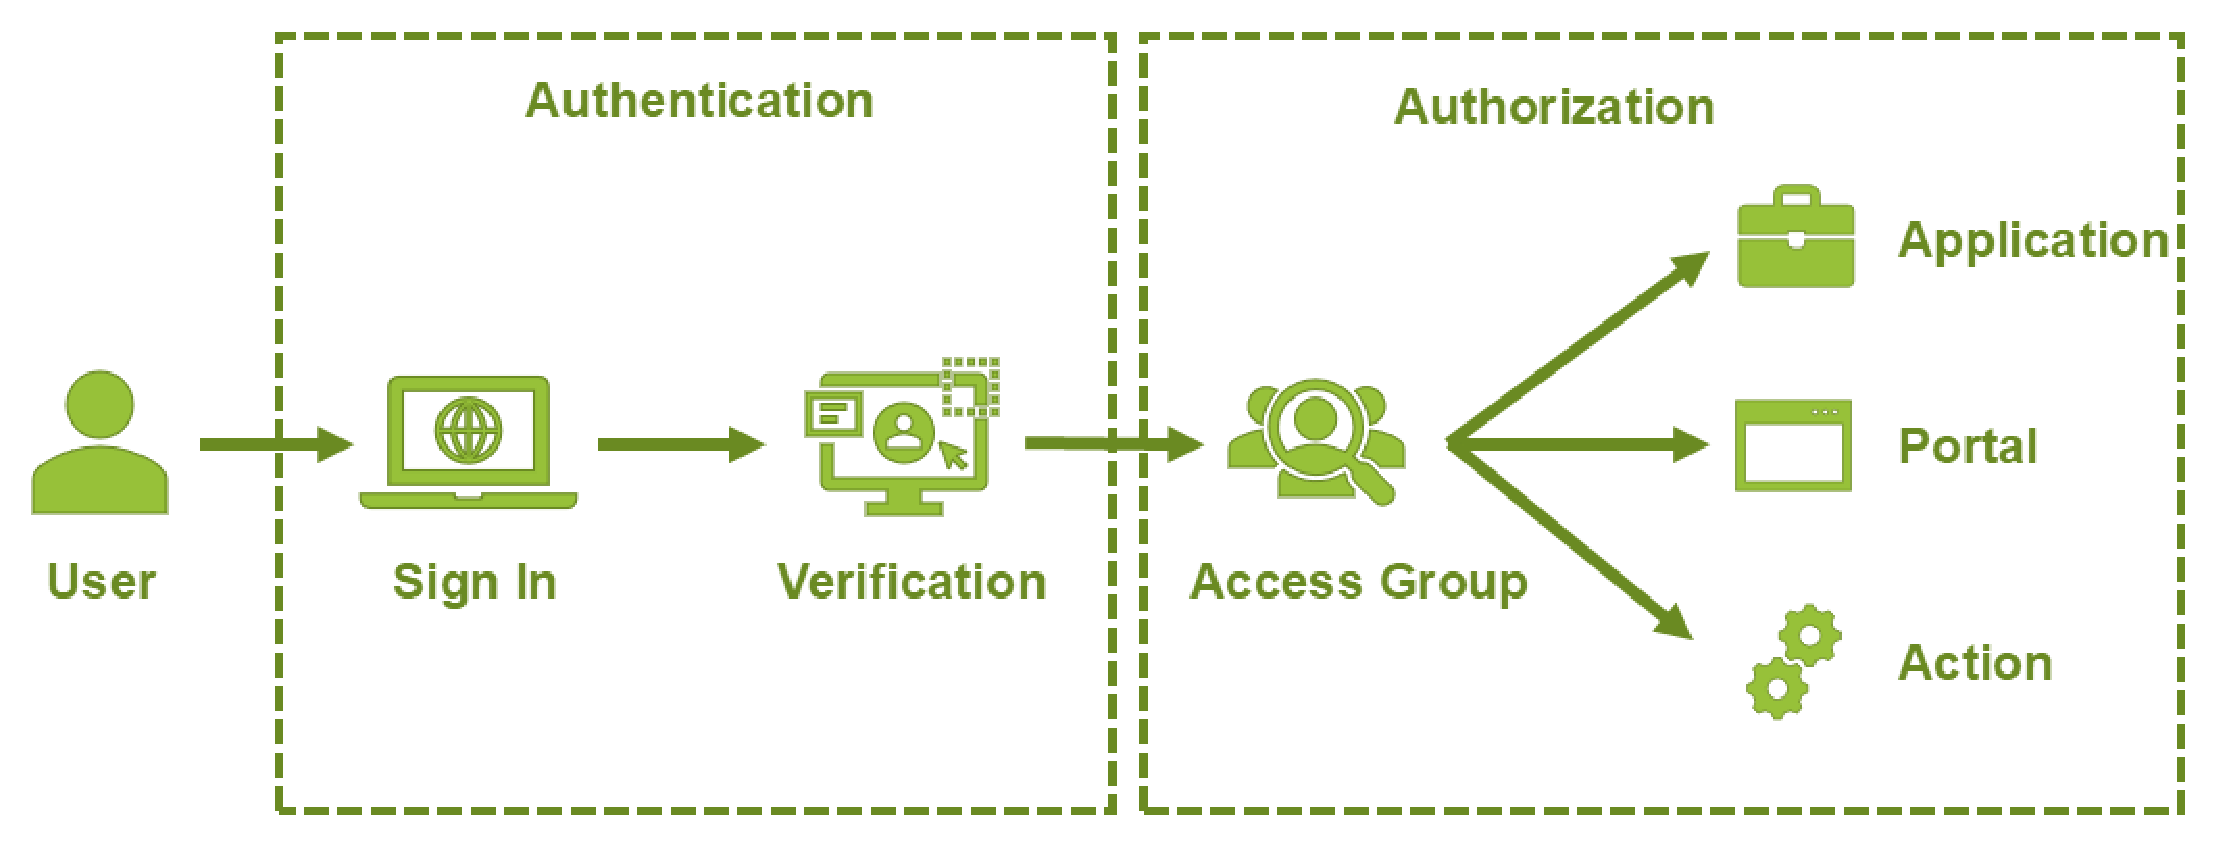
\includegraphics[width=1 \linewidth]{Thesis/Figures/Slide7.pdf}
\caption{\label{fig:Authentication and Authorization}Authentication and Authorization Flow \cite{r42}}
\end{figure}

\subsection{Keycloak for Authentication}

Keycloak is an open source identity and access management \abk{IAM}{Identity and Access Management} solution that provides a comprehensive approach for authentication in cloud-native architectures. The process begins when the client passes user data to Keycloak for authentication. After successful authentication, the application receives the access and ID tokens see \autoref{fig:Authentication}. Keycloak supports a wide range of authentication mechanisms, including multi-factor authentication MFA, SSO and social login, integrating seamlessly with modern applications and services. Keycloak simplifies the process of securing applications by providing built-in support for standards such as OAuth 2.0, OpenID Connect and SAML 2.0, which are crucial for verifying user identities and managing access across distributed systems. \cite{r38}

One of the primary advantages of Keycloak is its ability to act as a centralized authentication server, offering a single point of management for user identities and credentials. This centralized approach enhances security by enabling consistent application of authentication policies and reducing the complexity of managing credentials across multiple services. Keycloak also supports federated identity providers, allowing users to authenticate using their existing accounts from platforms like Google, Facebook and Microsoft Azure AD. This flexibility not only improves user experience by simplifying login processes but also strengthens security through robust identity verification methods \cite{keycloak_doc}. Moreover, Keycloak provides an intuitive administrative console for managing users, roles and permissions, making it easier for administrators to implement and enforce security policies across their cloud-native environments.


\captionsetup{justification=centering}
\begin{figure}[h]
\centering
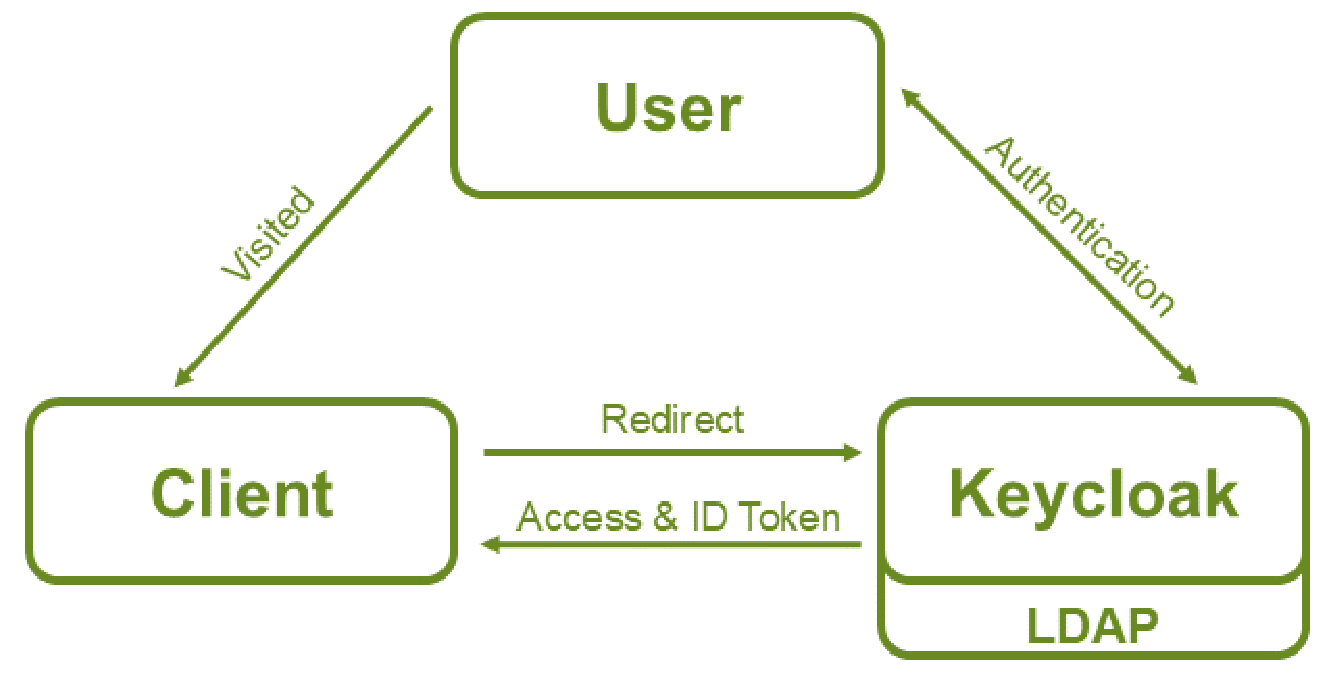
\includegraphics[width=0.65 \linewidth]{Thesis/Figures/Slide5.pdf}
\caption{\label{fig:Authentication}Keycloak Authentication Flow \cite{r45}}
\end{figure}



\textbf{Security Assertion Markup Language}

Security assertion markup language \abk{SAML}{Security Assertion Markup Language} is an open standard that uses XML encoding for security assertions and SAML messages as captured by the SAML specifications. It supports protocol bindings, which can be thought of as the insertion of SAML constructs into different transport layers, such as simple object access protocol \abk{SOAP}{Simple Object Access Protocol} over hypertext transfer protocol \abk{HTTP}{Hypertext Transfer Protocol}. In addition to profiles, SAML also describes in detail how a SAML assertion should be used in a communication protocol and also details security considerations when using SAML in different applications. An example is the artifact profile that ensures SSO of a user with a browser, a source site and a target site. In this protocol, there is a user who has already authenticated to the source site and returns, possibly by redirecting to the target site. The source site, which identifies the user's browser, stores the user's identity credential and sends the browser with the stored credential an identity credential and a SAML artifact, which is a reference to the stored credential, to the target site. When this artifact is received, the target site requests an assertion from the source site, which then verifies the user's authentication by providing the assertion to the target site, as shown in \autoref{fig:Security Assertion Markup Language (SAML)}. \cite{gross2003security}



\captionsetup{justification=centering}
\begin{figure}[h]
\centering
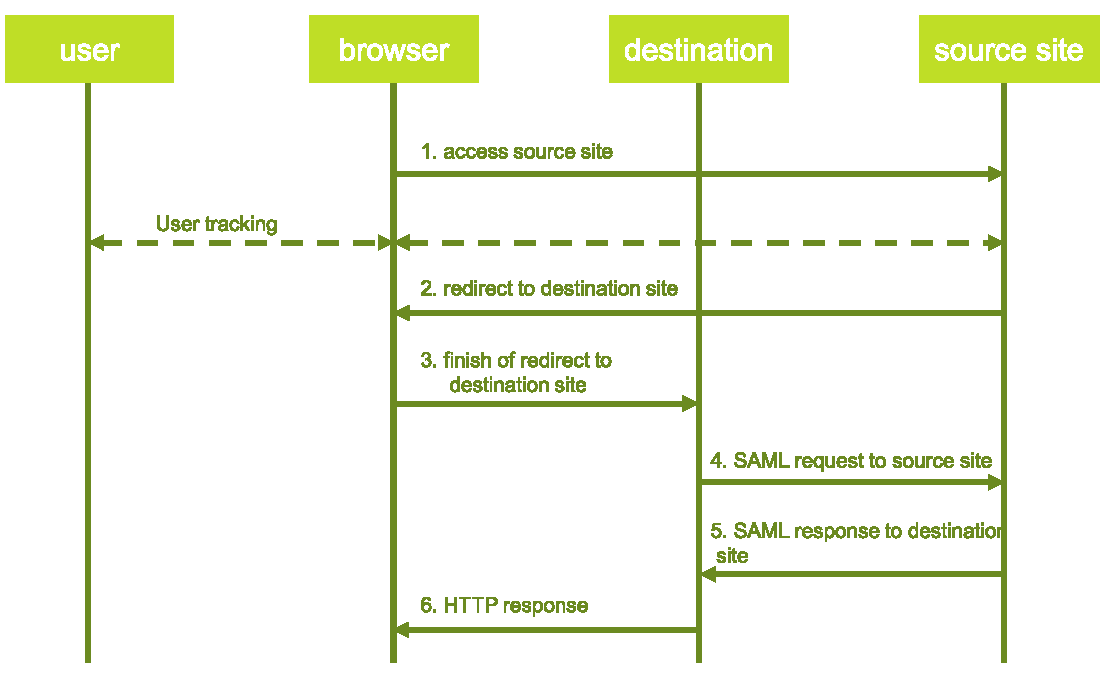
\includegraphics[width=0.75 \linewidth]{Thesis/Figures/Slide37.pdf}
\caption{\label{fig:Security Assertion Markup Language (SAML)}Authentication Flow of SAML \cite{gross2003security}}
\end{figure}

\clearpage

\textbf{Open Authorization}

Open Authorization \abk{OAuth}{Open Authorization} is an open standard that provides an efficient mechanism for users to use APIs in a standardized and secure way. The system allows users, known as resource owners, to allow third party applications, known as clients, to interact with their online resources on their behalf without having to share their credentials. The OAuth protocol consists of four primary components The resource server, which hosts the user's data. The client, which requests access to protected content from the resource server on behalf of the user and the authorization server, which authenticates the user and returns tokens that act as credentials for the client to access the resource server. In addition, the OAuth protocol allows end users to specify the level of access granted to applications, ensuring that only authorised applications can perform the required tasks. The authorization code flow is a key OAuth flow, often used for server side applications with a back-end server. In this flow, the client initiates an authorisation request by redirecting the user to the authorization server, which performs an authentication process and prompts the user for consent to grant access. Once the user has agreed, the authorisation server sends the required authorisation code back to the client via the user's browser or mobile application. The client then exchanges the code with the authorisation server in return for an access token, which is then used to access the relevant data held by the resource server on behalf of the user, as shown in \autoref{fig:OAuth 2.0}. This flow provides enhanced security by ensuring that access tokens are not exposed directly to the user but are securely handled by the clients backend server. The use of the authorization code flow facilitates secure and controlled access to user data across a broad spectrum of applications and platforms in accordance with the standards set out by OAuth. \cite{ranjbar2012authentication}
 

\captionsetup{justification=centering}
\begin{figure}[h]
\centering
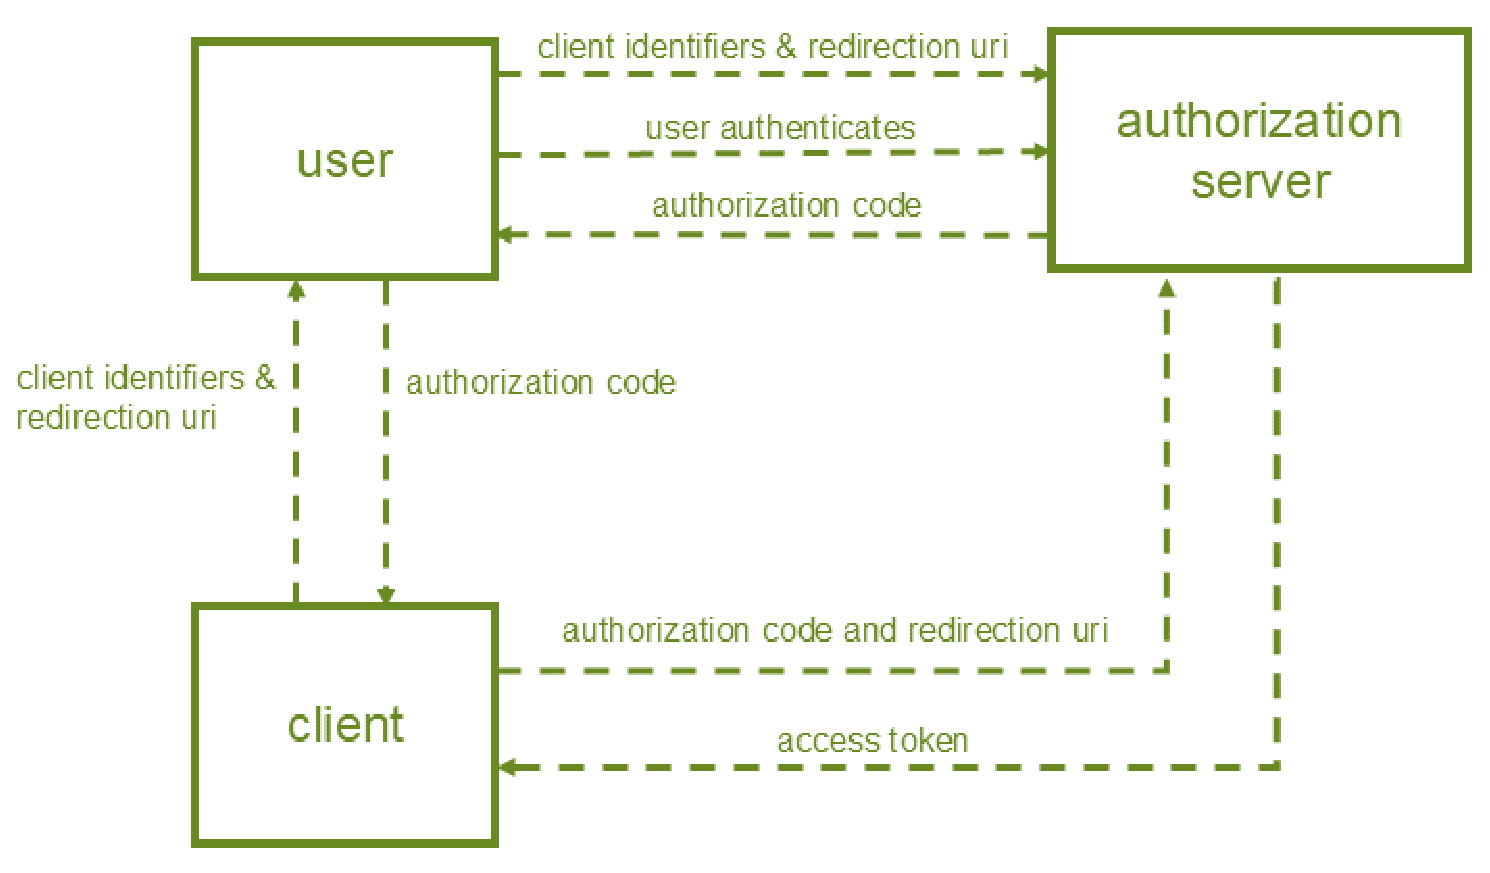
\includegraphics[width=1 \linewidth]{Thesis/Figures/Slide39.pdf}
\caption{\label{fig:OAuth 2.0}OAuth Authorization Flow \cite{ranjbar2012authentication}}
\end{figure}

\clearpage

\textbf{OpenID Connect}

OpenID Connect is a simple identity layer built on top of the OAuth 2.0 protocol that allows clients to verify the identity of end users based on authentication performed by an authorization server, also called an OpenID provider. It extends OAuth 2.0 by using authentication requests that include the OpenID scope, allowing the OpenID provider to issue ID tokens in the form of JSON web tokens \abk{JWT}{JSON Web Tokens} that contain information about the user's authentication. The protocol follows a flow where the client sends an authentication request to the OpenID provider, the OpenID provider verifies the end user and grants the permission. An access token is then returned by the OpenID provider. The client can use the access token to request additional information about the end user from the OpenID provider's UserInfo endpoint. The endpoint responds with user profile information. OpenID Connect thus extends OAuth 2.0 by adding a standardised way of providing authentication and identity information, making it interoperable and suitable for a wide range of web, mobile and API based applications. \autoref{fig:OIDC} shows the complete authentication protocol flow. \cite{openid-connect-core-1_0}


\captionsetup{justification=centering}
\begin{figure}[h]
\centering
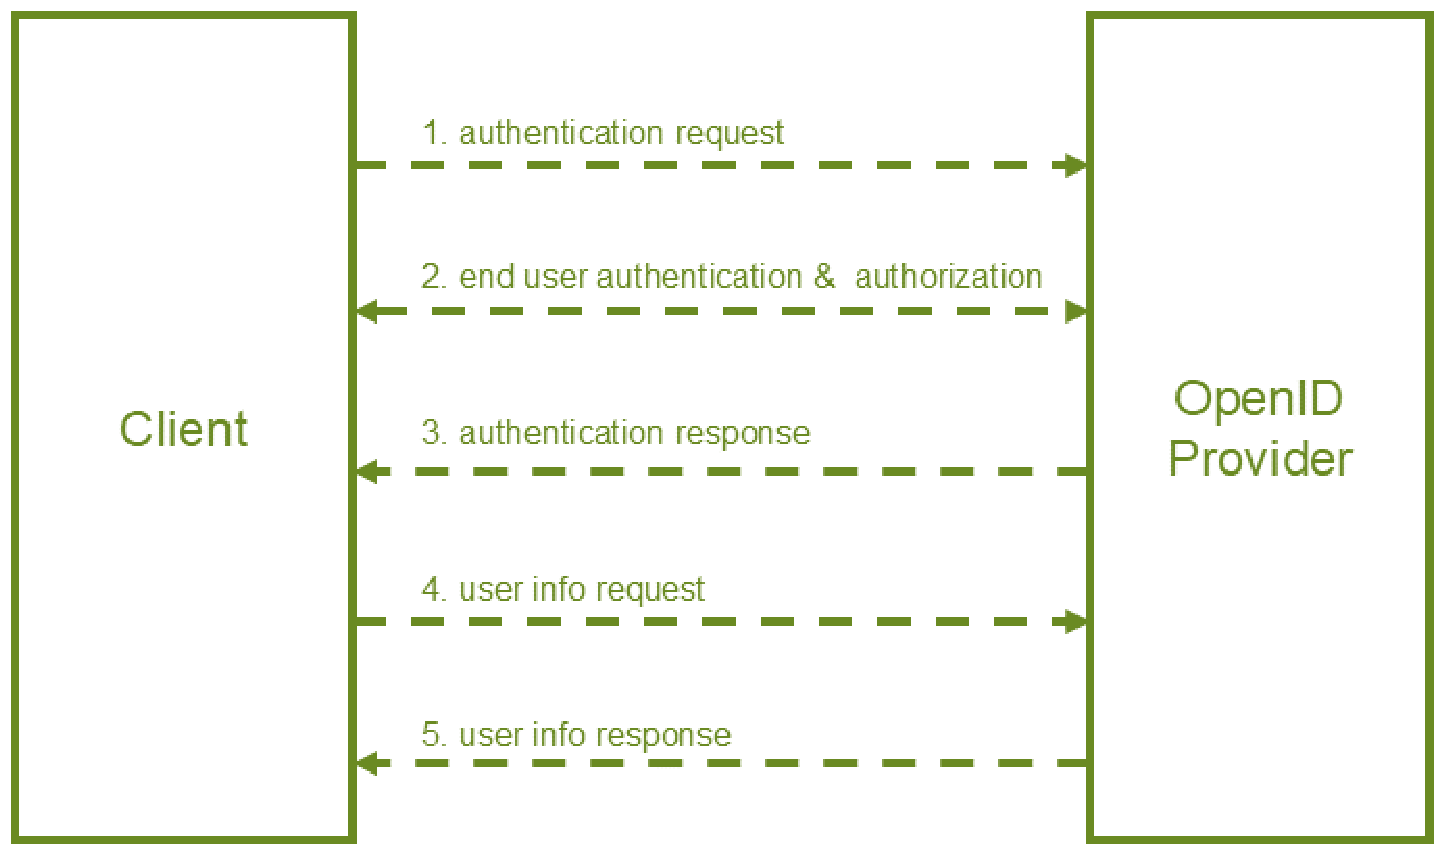
\includegraphics[width=0.9 \linewidth]{Thesis/Figures/Slide38.pdf}
\caption{\label{fig:OIDC}OpenID Connect Protocol \cite{openid-connect-core-1_0}}
\end{figure}

\subsection{Kubernetes Role-Based Access Control for Authorization}

RBAC is a comprehensive mechanism for managing authorization in cloud-native environments. It allows administrators to define and enforce policies using config files that dictate what actions users and services can perform within a Kubernetes cluster as shown in \autoref{fig:Authorization}. RBAC achieves this by assigning roles to users, groups, or service accounts and then binding these roles to specific permissions. This model simplifies the management of access control by organizing permissions based on roles rather than individual users, which is particularly beneficial in large and dynamic environments like those managed by Kubernetes. \cite{r40}
\clearpage

\captionsetup{justification=centering}
\begin{figure}[h]
\centering
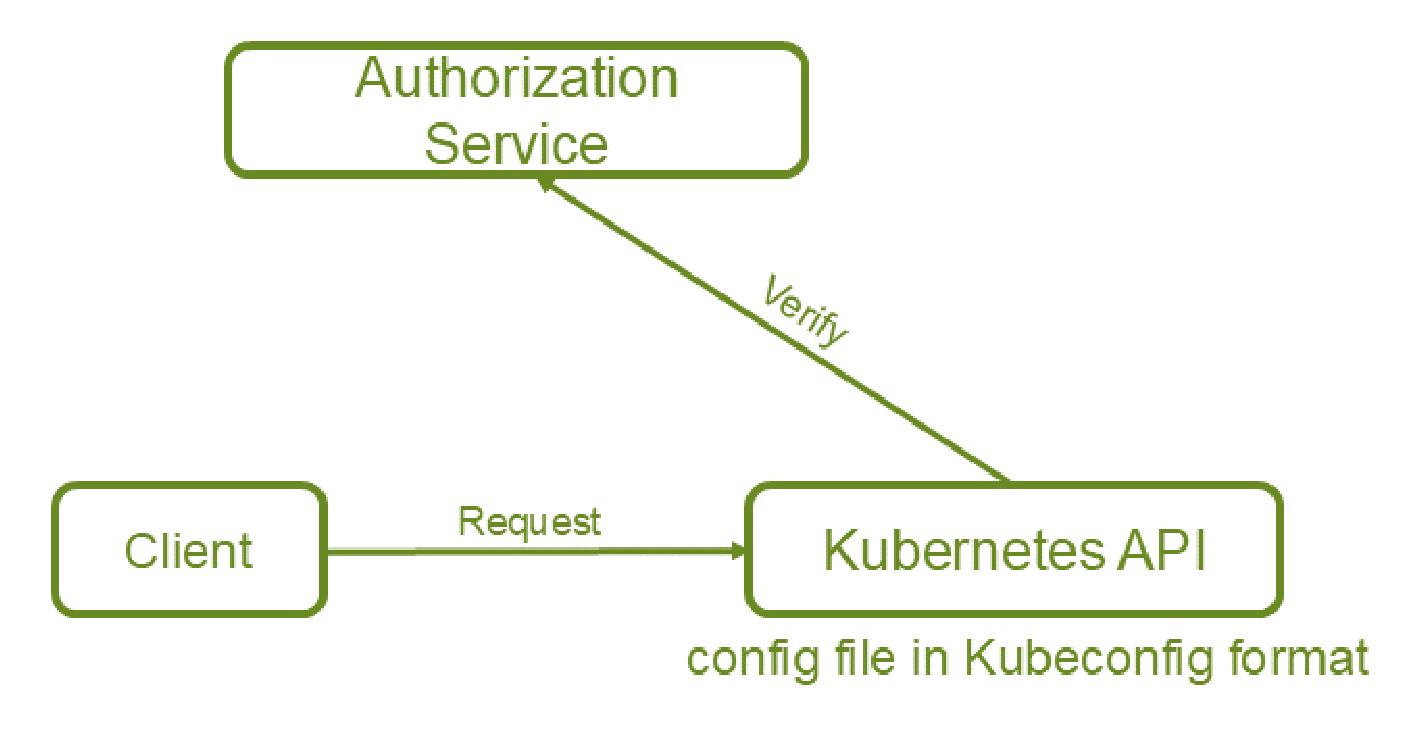
\includegraphics[width=0.7 \linewidth]{Thesis/Figures/Slide6.pdf}
\caption{\label{fig:Authorization}Authorization Request Flow \cite{r47}}
\end{figure}


\textbf{Components of Role-based Access Control:}

Roles, RoleBindings, ClusterRoles and ClusterRoleBindings are four components of RBAC. Roles and RoleBindings are namespace scoped allowing for fine-grained control over resources within the specific namespaces. ClusterRoles and ClusterRoleBindings on the other hand are cluster scoped allowing administrators to define global permissions that apply across all namespaces. This flexibility allows for precise and scalable access control management. By leveraging RBAC, organizations can ensure that users and services operate with the principle of least privilege, enhancing the security and stability of their cloud-native applications. Additionally, Kubernetes RBAC integrates seamlessly with other authentication mechanisms, such as OAuth 2.0 and OIDC , providing a comprehensive security solution that covers both authentication and authorization. \cite{Kubernetes_doc}

\textbf{User Accounts}

In Kubernetes, user accounts are identities assigned to human users, such as administrators, developers, or other team members, who need to access the Kubernetes cluster to perform tasks like development, maintenance, or administrative operations. These user accounts are managed outside of Kubernetes, typically by an identity provider and are used to authenticate and authorize access to the cluster resources. RBAC policies are applied to these user accounts to define what actions they can perform within the cluster, ensuring that access is restricted based on roles and responsibilities. \cite{rahasak_Kubernetes_rbac}


\textbf{Service Accounts}

Service accounts are identities specifically designed for software resources and processes that run within the Kubernetes environment. Unlike user accounts, service accounts are used by applications and processes, such as pods, to authenticate with the Kubernetes API server. Each namespace in Kubernetes comes with a default service account, which is automatically assigned to pods unless a different service account is specified. However, this default service account has minimal permissions. To grant more specific permissions or to have finer control over what an application or process can do within the cluster, custom service accounts can be created and managed using RBAC policies, allowing secure and restricted access for the applications running in the Kubernetes environment. \cite{rahasak_Kubernetes_rbac}

\clearpage

\textbf{Role}

A role in Kubernetes is a namespaced resource that defines a set of permissions specific to a particular namespace. When you create a role, you need to specify the namespace it belongs to, as its permissions are limited to that namespace only. Roles are used to grant access to resources such as pods, services or config maps within a particular namespace. For example, a role might only allow a user or service account to read, watch and list pods within the default namespace. This is achieved by defining the permissions in a role configuration. In the \autoref{listingsnippet:1} code snippet, the Role named \texttt{pod-reader} grants read-only access to pods in the \texttt{default} namespace. The rules section specifies that the role will allow the get, watch and list actions to be performed on pods, but only within this particular namespace. \cite{Kubernetes_doc}


\listingsnippet{Role Example \cite{Kubernetes_doc}}{

\vspace{0.3cm}

\hspace{0.25cm} \texttt{apiVersion: rbac.authorization.k8s.io/v1}

\hspace{0.25cm} \texttt{kind: Role}

\vspace{0.3cm}

\hspace{0.25cm} \texttt{metadata:}

\hspace{1cm} \texttt{namespace: default}

\hspace{1cm}name: \texttt{pod-reader}

\vspace{0.3cm}

\hspace{0.25cm} \texttt{rules:}

\hspace{0.25cm} \texttt{- apiGroups: [""]}

\hspace{1cm}  \texttt{resources: ["pods"]}
  
\hspace{1cm}  \texttt{verbs: ["get", "watch", "list"]}

\vspace{0.3cm}

}


\textbf{ClusterRole}

In Kubernetes, the ClusterRole is a non-namespaced resource, meaning it has cluster wide scope. ClusterRoles are more versatile than Roles because they can define permissions not only for cluster scoped resources, such as nodes, but also for namespaced resources across all namespaces. ClusterRoles can be used to grant broad permissions, such as reading secrets in any namespace or accessing non resource 
\abk{URL}{Uniform Resource Locator}. For instance, the following ClusterRole configuration grants read access to secrets across all namespaces. In code snippet \autoref{listingsnippet:2}, the ClusterRole named \texttt{secret-reader} allows the get, watch and list actions on secrets, enabling the user or Service Account to read secrets in any namespace. Since ClusterRoles are cluster scoped, they provide a more flexible and powerful way to manage permissions across the entire Kubernetes cluster. \cite{Kubernetes_doc}

\listingsnippet{ClusterRole Example \cite{Kubernetes_doc}}{

\vspace{0.3cm}

\hspace{0.25cm} \texttt{apiVersion: rbac.authorization.k8s.io/v1}

\vspace{0.3cm}

\hspace{0.25cm} \texttt{kind: ClusterRole}

\vspace{0.3cm}

\hspace{0.25cm} \texttt{metadata:}

\hspace{1cm}\texttt{name: secret-reader}

\vspace{0.3cm}

\hspace{0.25cm} \texttt{rules:}

\hspace{0.25cm} \texttt{- apiGroups: [""]}

\hspace{1cm}\texttt{resources: ["secrets"]}

\hspace{1cm}\texttt{verbs: ["get", "watch", "list"]}

\vspace{0.3cm}
}

\textbf{RoleBinding}

A RoleBinding in Kubernetes is used to associate a Role with one or more users, groups, or service accounts within a specific namespace. This means that the permissions defined in the Role are granted to the specified subjects, but only within the namespace where the RoleBinding is created. For example, you might have a RoleBinding that grants a \texttt{pod-reader} role to a user in the namespace named \texttt{namespace1}, allowing her to read pod information only in that namespace as shown in the \autoref{fig:RoleBinding}. RoleBindings can also reference ClusterRoles to apply cluster scoped permissions to resources within a single namespace. This flexibility allows administrators to define common roles across the cluster and then apply them in different namespaces using RoleBindings. \cite{Kubernetes_doc}



\captionsetup{justification=centering}
\begin{figure}[h]
\centering
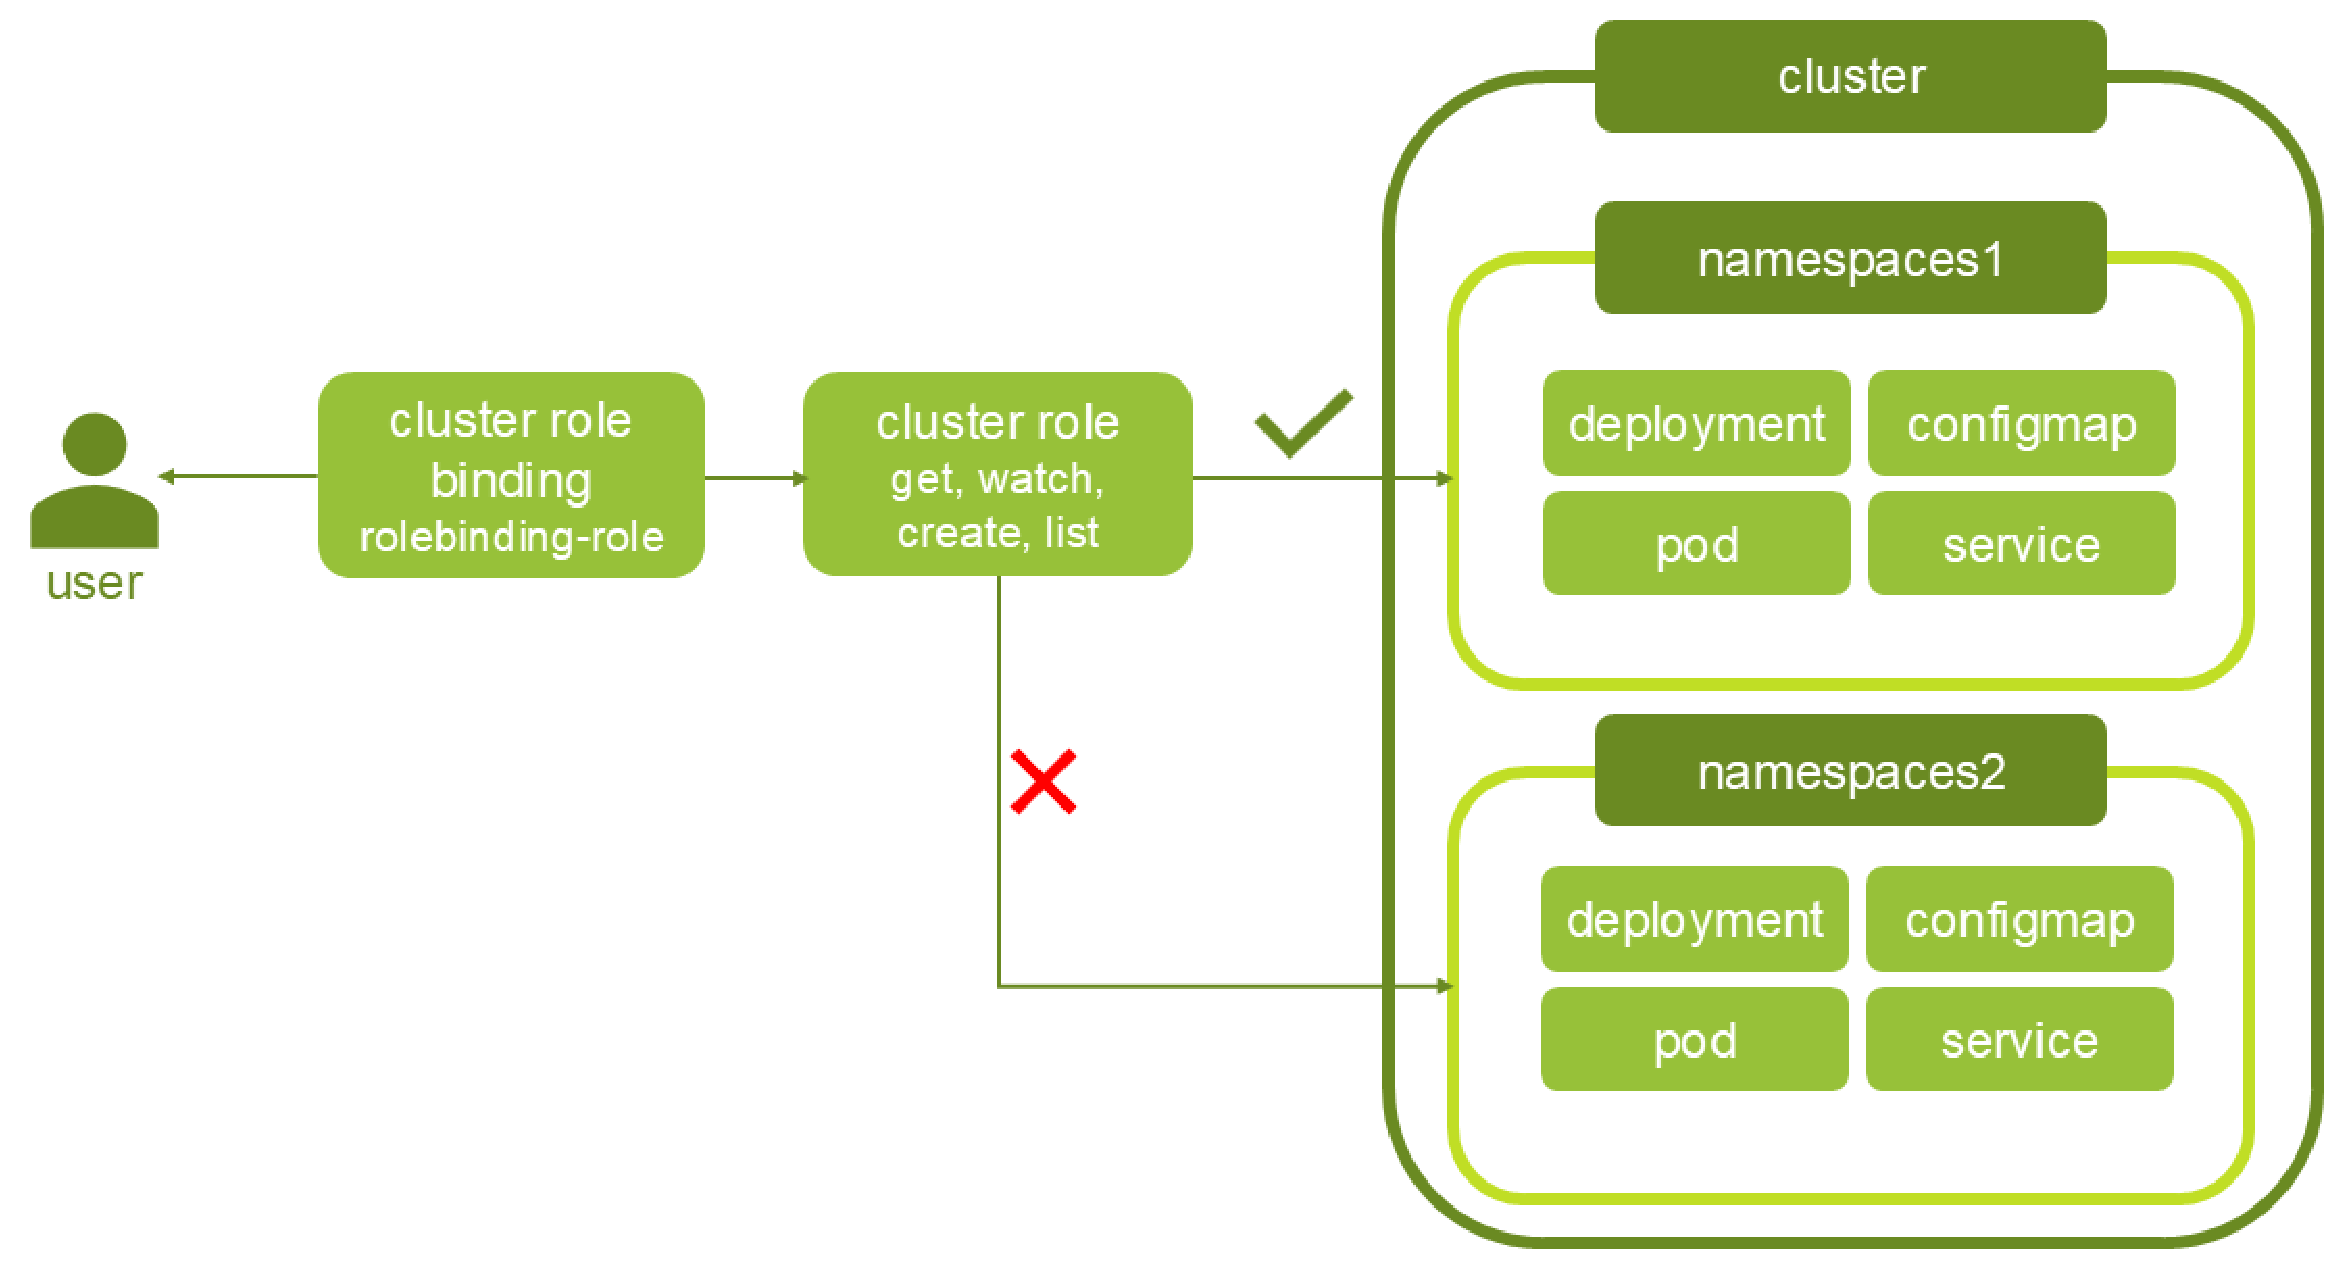
\includegraphics[width=1 \linewidth]{Thesis/Figures/Slide41.pdf}
\caption{\label{fig:RoleBinding}RoleBinding \cite{rahasak_Kubernetes_rbac}}
\end{figure}

\clearpage

\textbf{ClusterRoleBinding}

A ClusterRoleBinding, on the other hand, grants permissions cluster wide by associating a ClusterRole with one or more users, groups, or service accounts across the entire Kubernetes cluster. Unlike RoleBindings, which are confined to a single namespace, ClusterRoleBindings apply the permissions defined in a ClusterRole to all namespaces or to cluster scoped resources, as illustrated in the \autoref{fig:ClusterRoleBinding}. This makes ClusterRoleBindings ideal for granting broad access, such as allowing a group of managers to read secrets across all namespaces. Once a ClusterRoleBinding is created, it cannot be modified to reference a different role, if a change is needed, the binding must be deleted and recreated to ensure that the new roles permissions are intentionally granted to the subjects. \cite{Kubernetes_doc}


\captionsetup{justification=centering}
\begin{figure}[h]
\centering
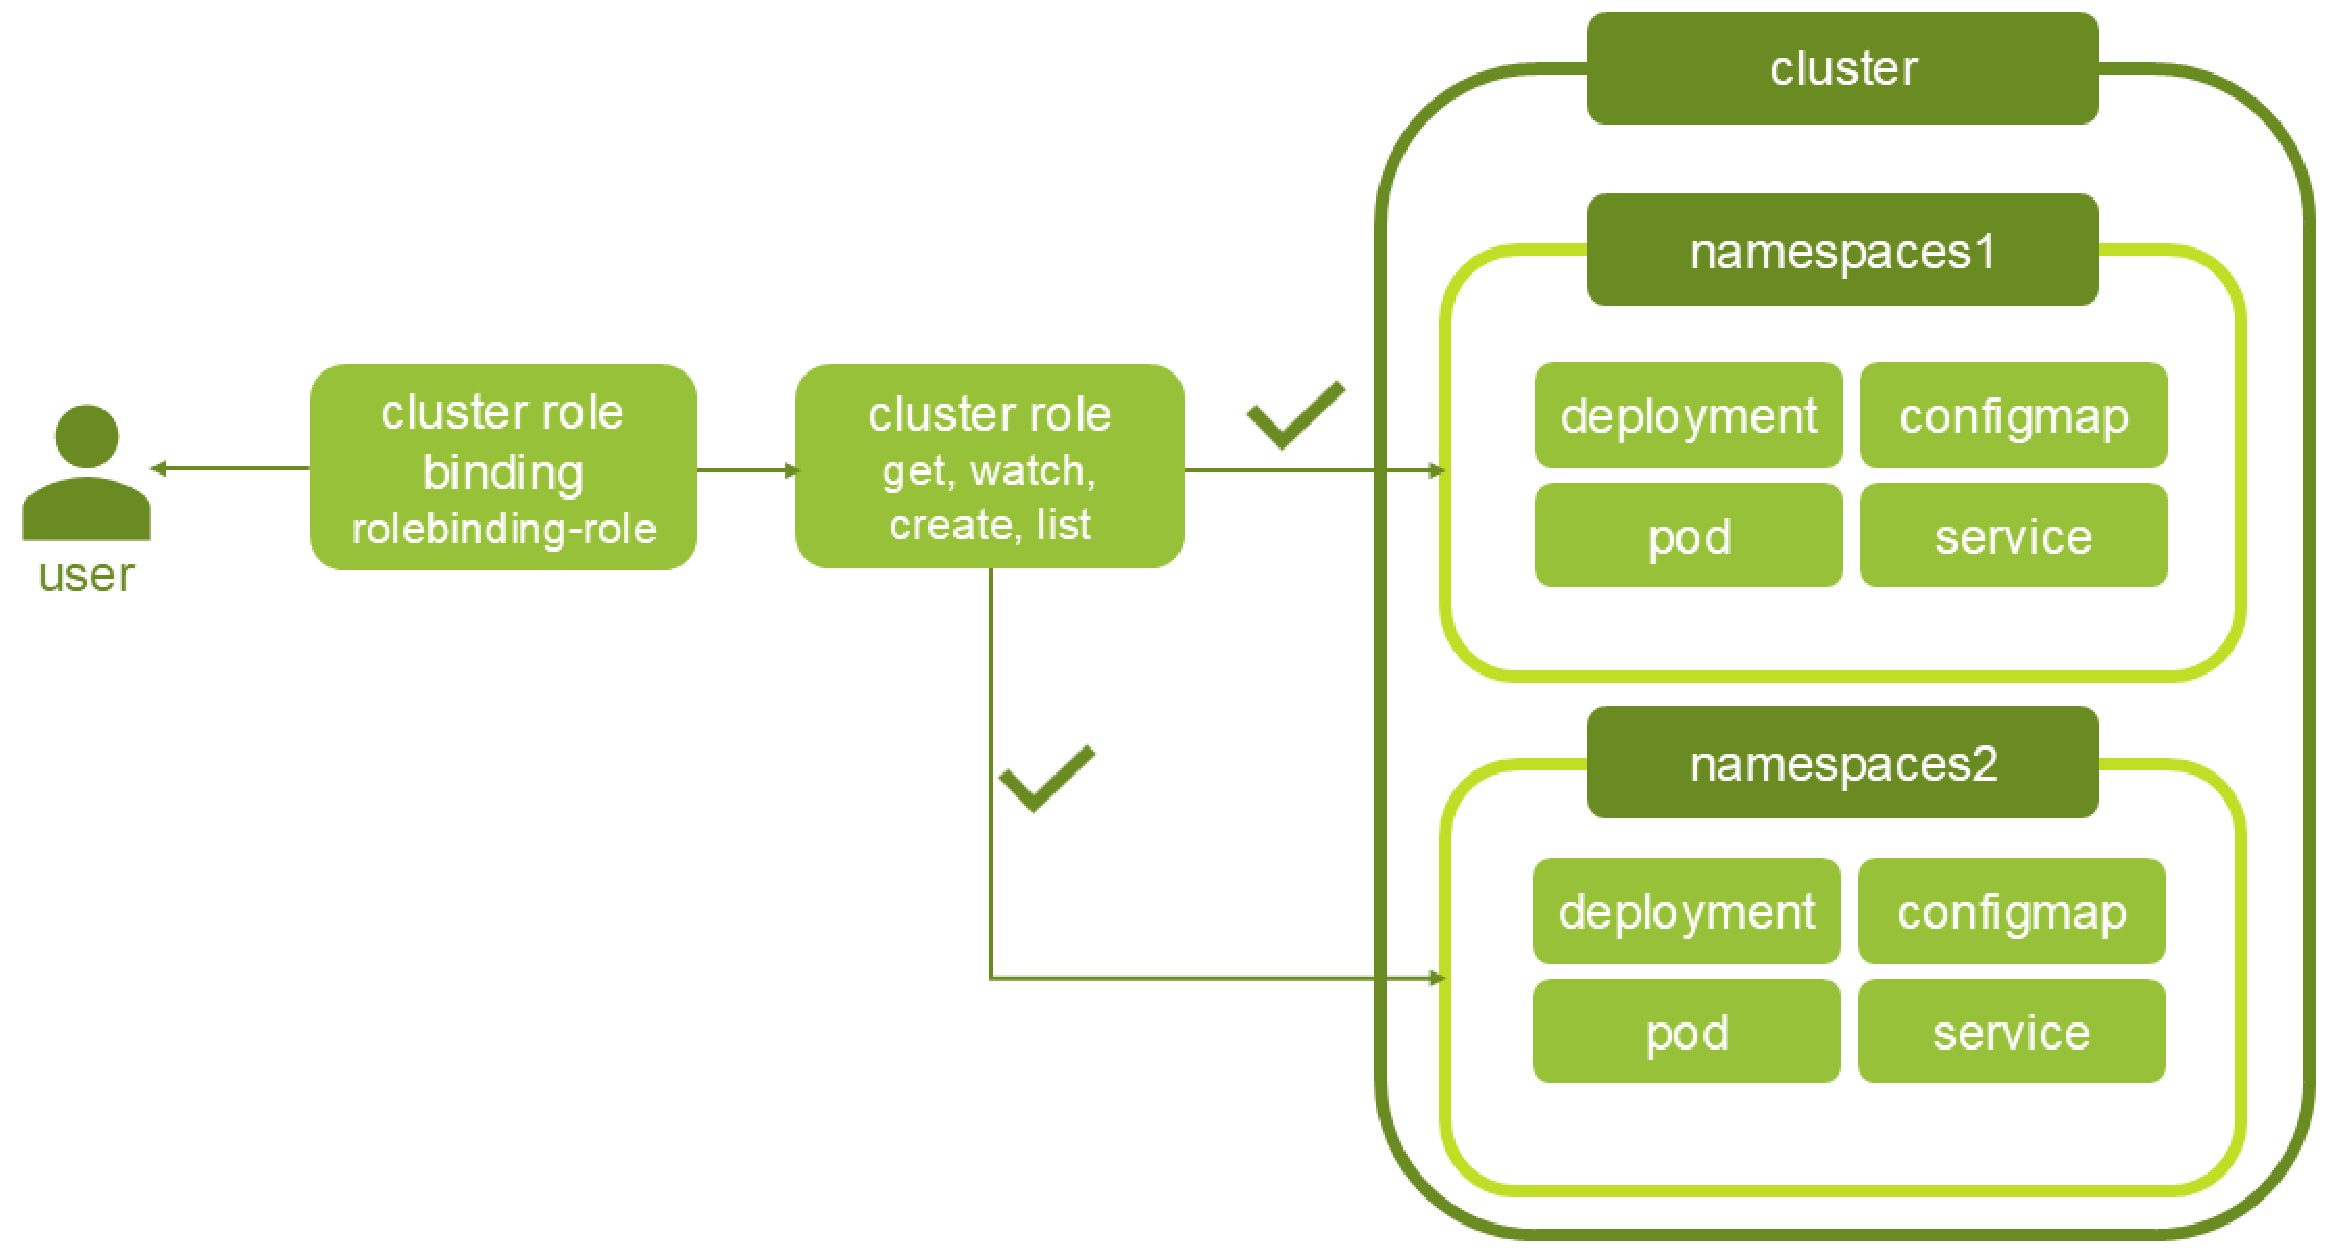
\includegraphics[width=1 \linewidth]{Thesis/Figures/Slide42.pdf}
\caption{\label{fig:ClusterRoleBinding}ClusterRoleBinding \cite{rahasak_Kubernetes_rbac}}
\end{figure}

\section{Scalable and Distributed Architecture for AI Models}

This section describes scalable and distributed architectures for AI models, focusing on concepts such as distributed and parallel computing, batch processing and frameworks that support large-scale workloads. It explains core architectural components, cluster management and autoscaling techniques to enable efficient model training and deployment.

\subsection{Distributed Computing}

Distributed computing is a system where multiple independent entities, often called nodes, collaborate to solve problems or tasks by sharing resources and information. These nodes operate in different physical or virtual locations, each potentially having its own hardware, software and tasks. Despite their independence, these nodes must coordinate their actions to achieve a common goal. This coordination involves managing communication between nodes, ensuring the system remains functional even if some nodes fail and optimizing the distribution of tasks to improve efficiency and performance as shown in \autoref{fig:Distributed Computing}. A defining characteristic of distributed computing is the diversity in how these systems are structured and operate. Nodes may work synchronously or asynchronously, communicate through message passing or shared memory. The challenges in distributed computing include managing communication costs, ensuring fault tolerance, coordinating tasks effectively and addressing uncertainty due to the lack of global knowledge among nodes. As a result, distributed computing is a complex and dynamic field, encompassing a wide range of models and techniques to address the varying needs and constraints of different applications. \cite{podc_roger_2015}

\captionsetup{justification=centering}
\begin{figure}[h]
\centering
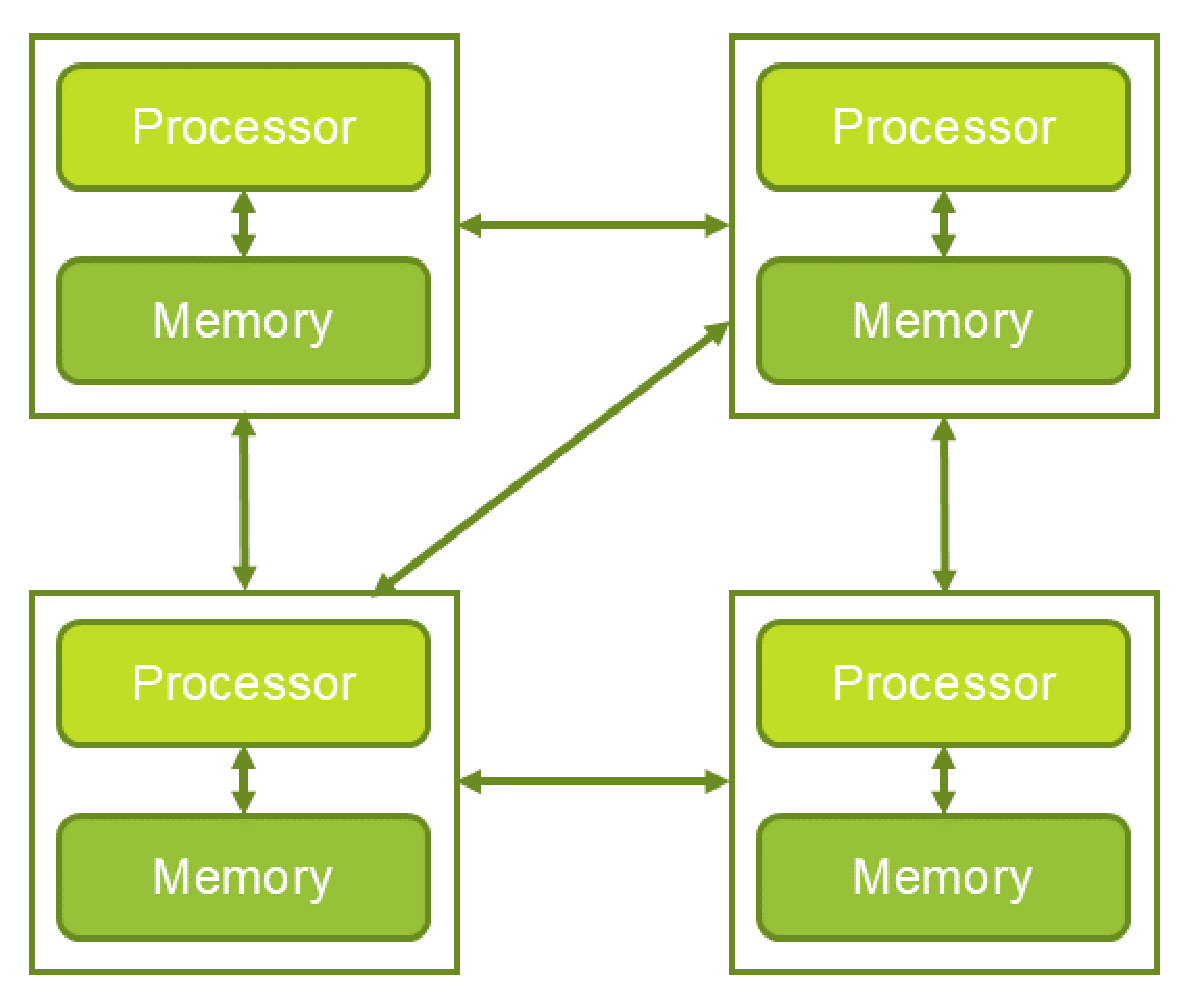
\includegraphics[width=0.7 \linewidth]{Thesis/Figures/Slide43.pdf}
\caption{\label{fig:Distributed Computing}Distributed Computing \cite{parallel_vs_distributed}}
\end{figure}

\subsection{Parallel Computing}

Parallel processing involves performing multiple tasks at the same time by using multiple processors, known as CPUs. This method is essential for handling complex problems that exceed the capabilities of traditional sequential computing systems. By dividing a task into smaller sub tasks through techniques such as divide and conquer and assigning these sub tasks to different processors, parallel processing significantly enhances computational efficiency and performance. This approach allows for the concurrent handling of diverse processes, which leads to a substantial increase in computing power compared to single processor systems as shown in \autoref{fig:Parallel Computing}. The push towards parallel processing is driven by several factors, including the growing computational demands of scientific and business applications. Sequential processors are reaching their performance limits due to physical constraints and the diminishing returns of hardware improvements like pipelining architectures. While vector processing works well for certain scientific applications, it is less effective for more general use cases. However, advances in parallel processing technology and networking have made it a viable and commercially exploitable solution, facilitating the development of more powerful and versatile computing systems. \cite{buyya2012microkernel}

\captionsetup{justification=centering}
\begin{figure}[h]
\centering
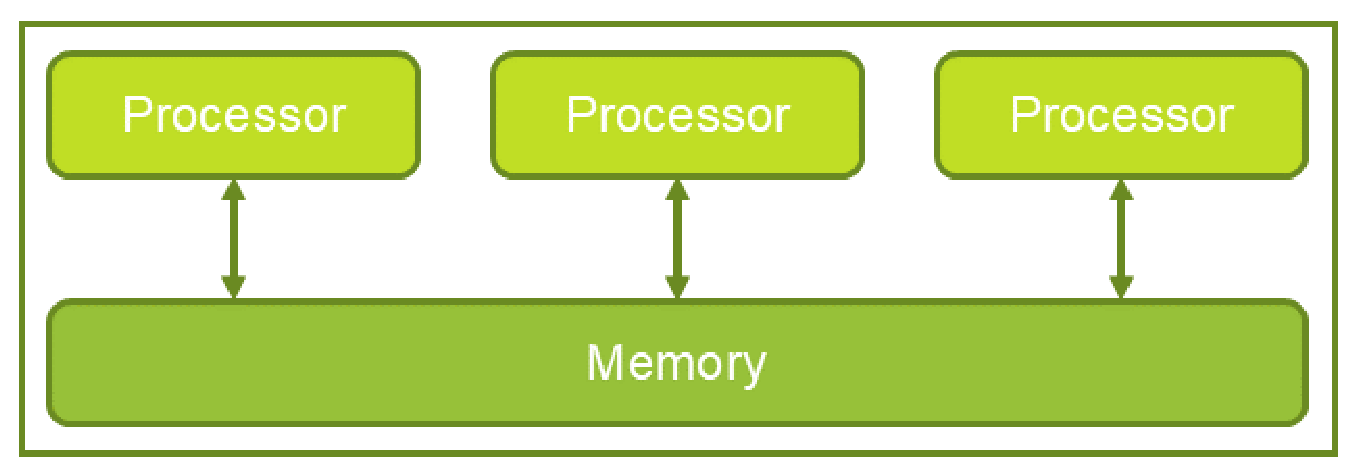
\includegraphics[width=0.9 \linewidth]{Thesis/Figures/Slide44.pdf}
\caption{\label{fig:Parallel Computing}Parallel Computing \cite{parallel_vs_distributed}}
\end{figure}



\subsection{Batch Processing}
Batch processing is a computing technique where a set of tasks or jobs is processed in a group or batch rather than individually as shown in \autoref{fig:Batch Processing}. This method is particularly efficient for handling large volumes of data or executing repetitive tasks with minimal human intervention. By queuing jobs and processing them sequentially, batch processing can optimize resource utilization and improve overall system throughput. For instance, in large-scale data analysis, batch processing allows for the aggregation and analysis of massive datasets in a structured and efficient manner, reducing the overhead associated with constant task switching and manual processing. The primary advantages of batch processing include its ability to perform operations during off peak hours, which minimizes the impact on system performance during peak times. Additionally, it supports automation and scheduling, which can significantly enhance productivity and reduce human error \cite{silberschatz2011database}. However, batch processing can introduce latency because jobs are only processed at scheduled intervals, which may not be suitable for applications that require real-time data processing. As a result, balancing batch processing with real-time systems is critical to optimising performance in different computing environments. \cite{tanenbaum2009modern}

\captionsetup{justification=centering}
\begin{figure}[h]
\centering
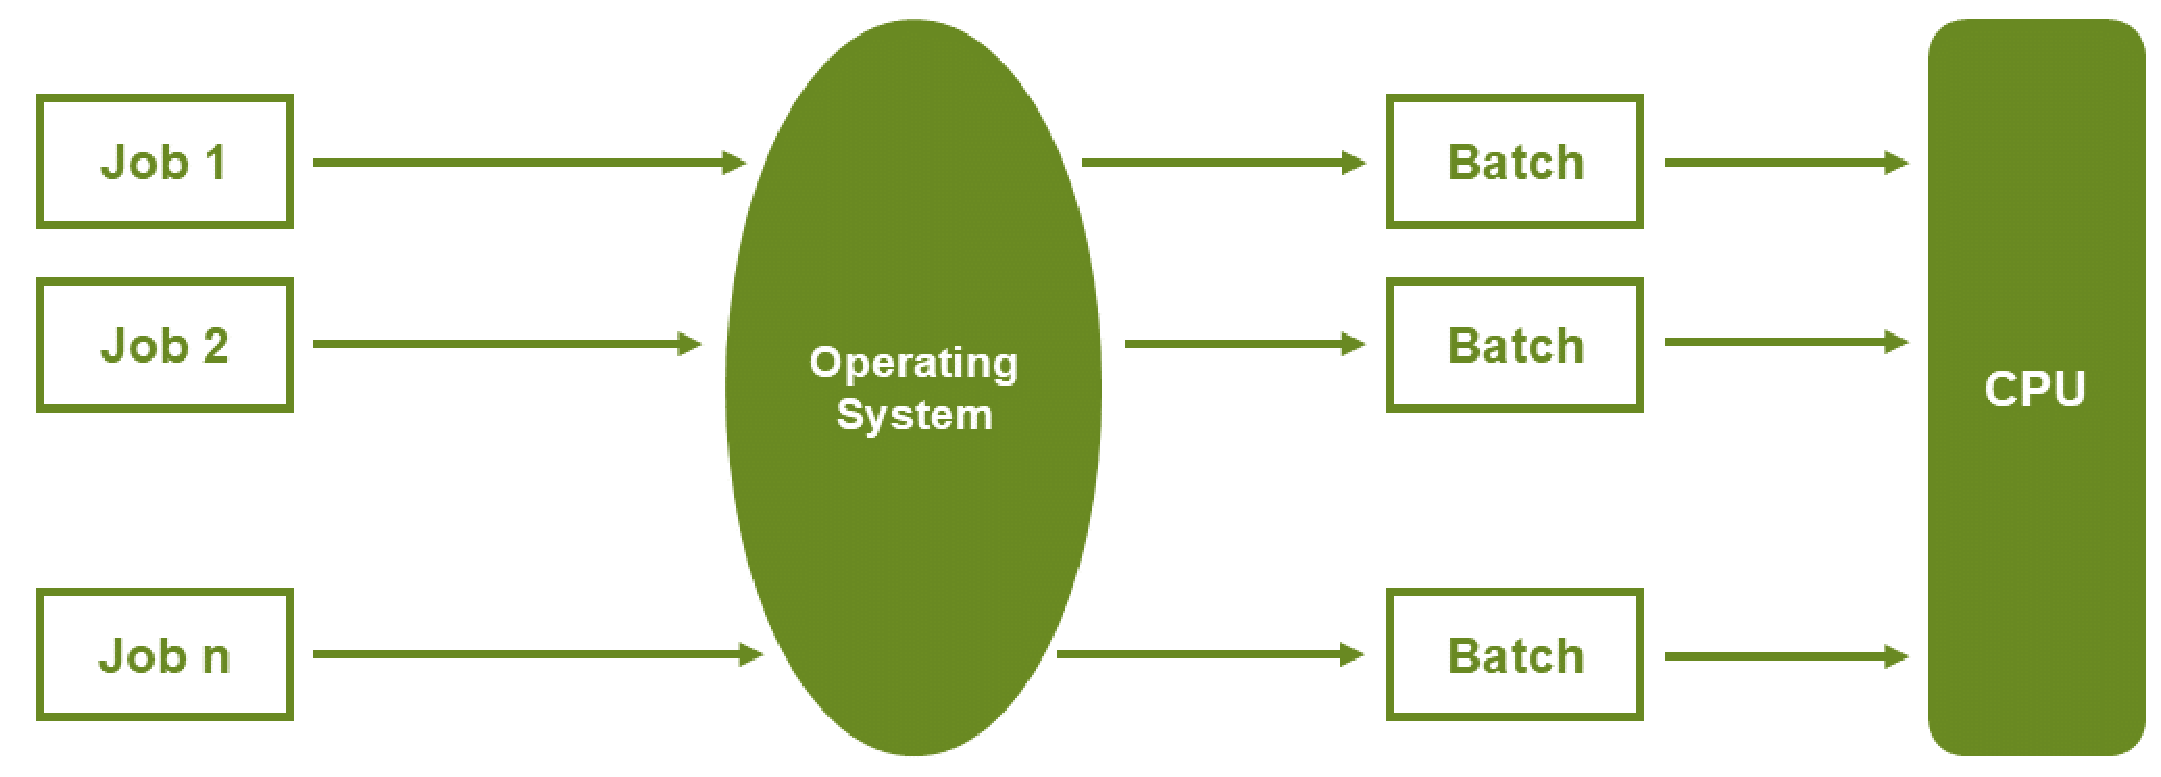
\includegraphics[width=0.9 \linewidth]{Thesis/Figures/Slide45.pdf}
\caption{\label{fig:Batch Processing}Batch Processing \cite{batch_processing_os}}
\end{figure}

\subsection{Ray Framework}

Ray is an open source framework that makes it easy to scale AI and ML applications with minimal effort. It enables developers to efficiently build distributed applications using a simple, flexible API. Ray core features include parallel and distributed computation, enabling the scaling of machine learning models across multiple nodes with minimal code changes. It supports a range of libraries based on Ray core, such as Ray data for distributed data processing, Ray train for ML and DL model training, Ray tune for hyperparameter tuning as shown in \autoref{fig:Ray Framework}. These features make Ray particularly advantageous for AI model deployment and scaling, as it abstracts the complexity of distributed computing, allowing researchers and engineers to focus more on model development rather than the underlying infrastructure. \cite{anyscale_blog}

The primary advantages of using Ray for AI model deployment include its ease of use, flexibility and robust performance. Ray architecture supports both stateless and stateful computations, enabling it to handle a wide variety of workloads. Additionally, Ray offers fault tolerance and dynamic resource management, which are critical for maintaining performance and reliability in large-scale AI systems. These capabilities are particularly beneficial for scaling AI models, as they allow for seamless integration and execution across diverse computational environments, from single machines to large clusters. Ray's flexibility and efficiency make it an optimal selection for the development and deployment of scalable AI applications. \cite{ray_doc}


\captionsetup{justification=centering}
\begin{figure}[h]
\centering
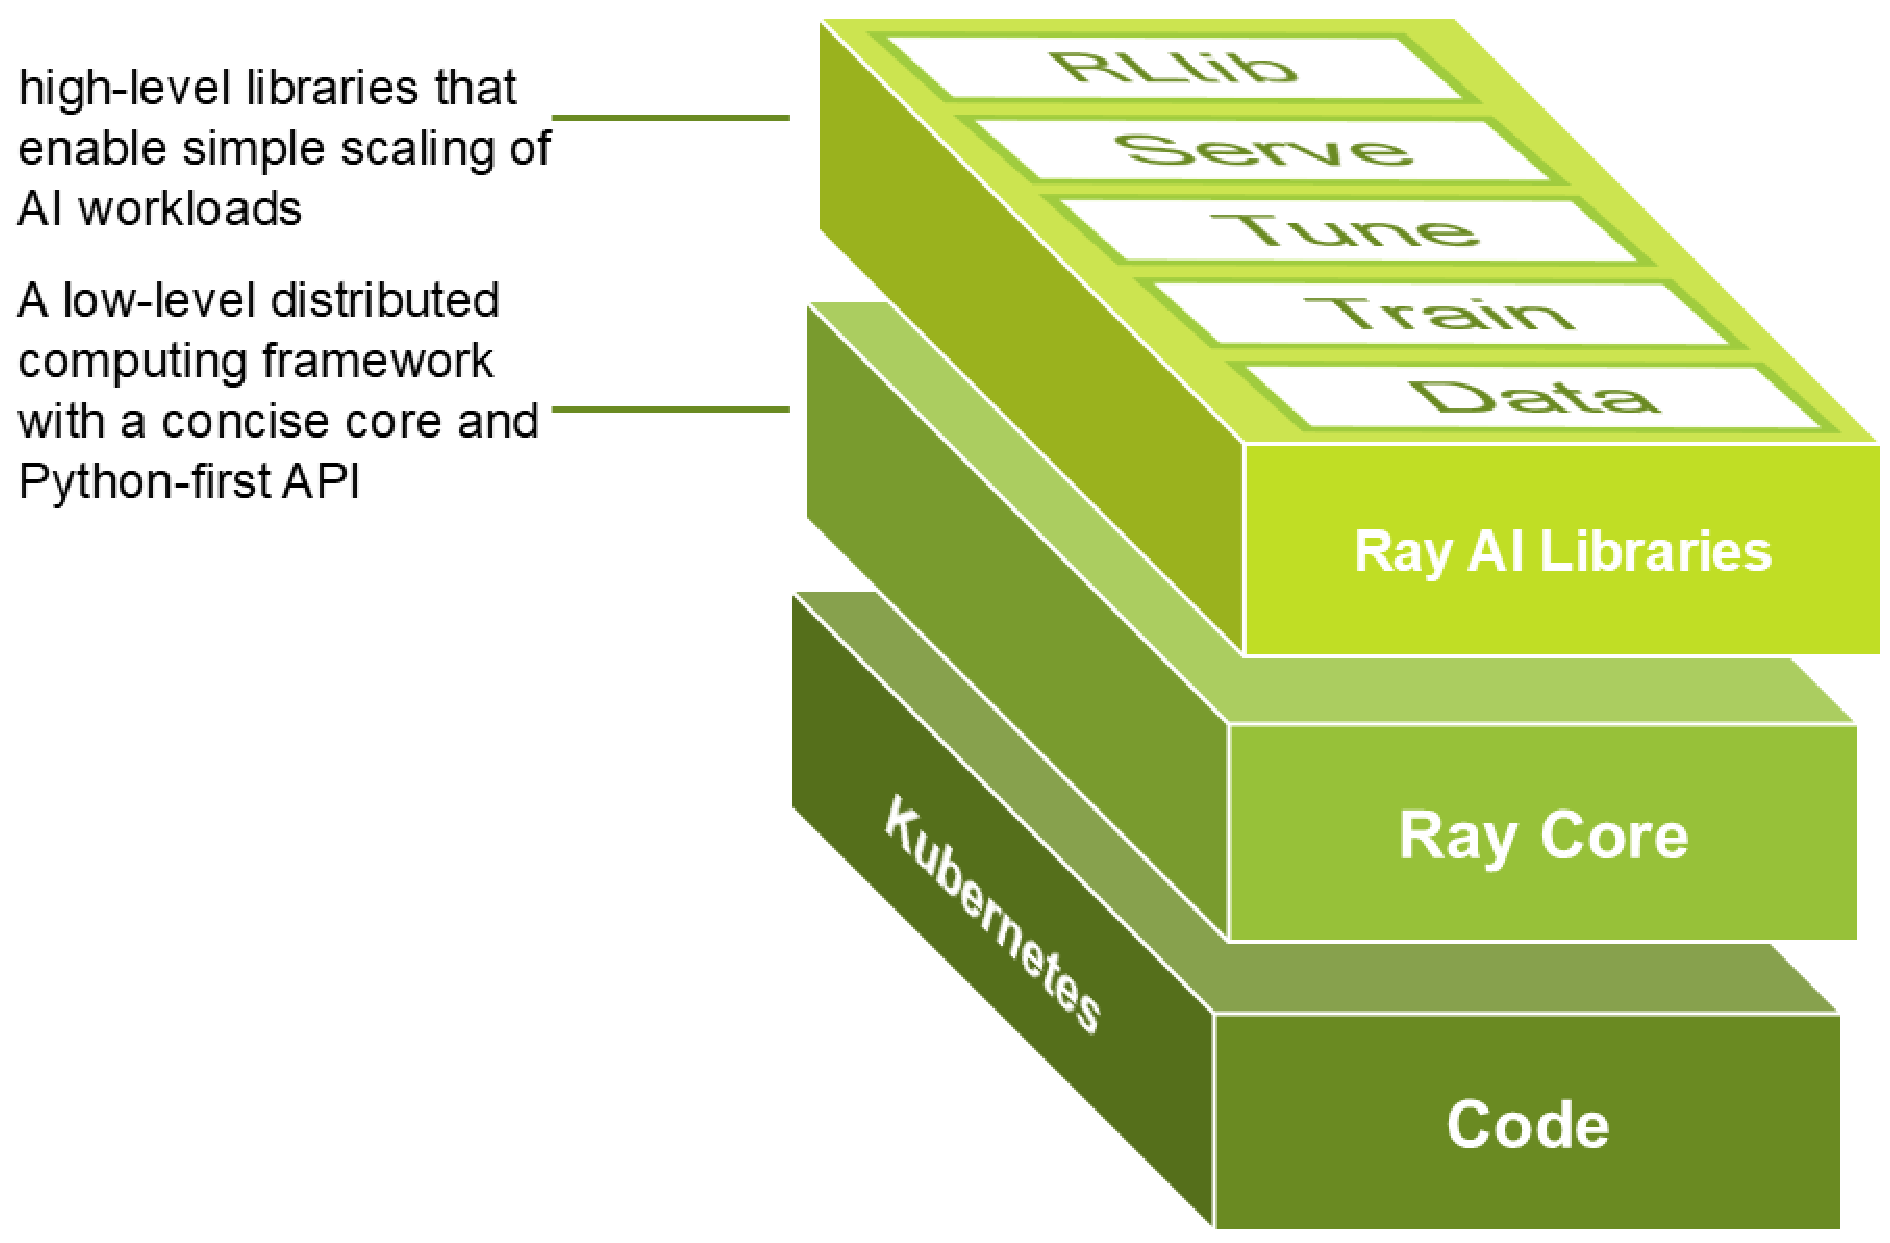
\includegraphics[width=1 \linewidth]{Thesis/Figures/Slide31.pdf}
\caption{\label{fig:Ray Framework}Ray Framework \cite{ray_doc}}
\end{figure}


\subsection{Ray Architecture}

Ray architecture is consist of two types of nodes, the head nodes and the worker nodes. A Ray head node is defined as a compute instance that executes the Ray components. Where a worker node is responsible for executing tasks based on Python process that is embedded within the head node. The head node is responsible for managing metadata and can be accessed by other nodes within the cluster. The head node contains a global control store, which provides assistance to workers in locating large objects within the cluster. The head node is furnished with a Raylet, comprising a scheduler for the administration of resources and an object store for the management of memory and state. The structure of the worker node is analogous to that of the head node, although it lacks the global control store and driver process. Each worker node is furnished with its own Raylet, which is responsible for the supervision of resource management and the administration of the object store as shown in \autoref{fig:Ray Architecture}. The distributed object store enables the sharing of large objects among worker nodes. The location of these objects can be determined by utilising the metadata stored within the global control store. Ray facilitates dynamic scaling, allowing for the addition or removal of worker nodes during the execution of an application. \cite{r34}



\captionsetup{justification=centering}
\begin{figure}[h]
\centering
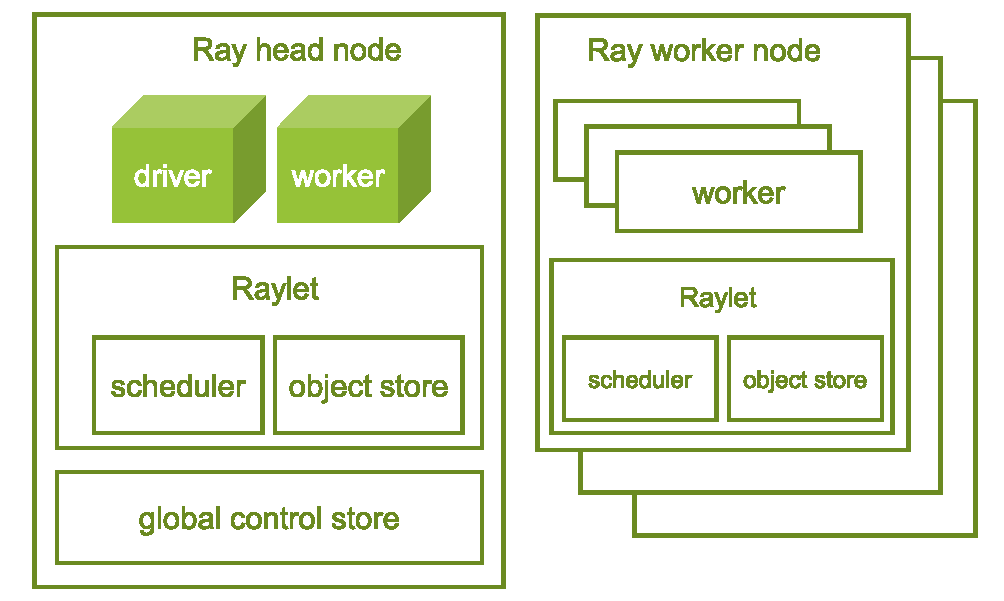
\includegraphics[width=1 \linewidth]{Thesis/Figures/Slide15.pdf}
\caption{\label{fig:Ray Architecture}Ray Architecture \cite{r34}}
\end{figure}


\subsection{Ray Cluster}

Ray enables seamless scaling of workloads from a single laptop to a large cluster. To run Ray applications across multiple nodes, deploying a Ray cluster is necessary. A Ray cluster comprises a head node and multiple worker nodes, which can be configured to autoscale based on the resource demands of the applications. This flexibility allows Ray clusters to efficiently handle varying workloads by scaling up or down as required and shown in \autoref{fig:Ray Cluster}.
A Ray cluster with two worker nodes. Each node runs Ray helper processes to facilitate distributed scheduling and memory management. The head node runs additional control processes. \cite{ray_doc}


\captionsetup{justification=centering}
\begin{figure}[h]
\centering
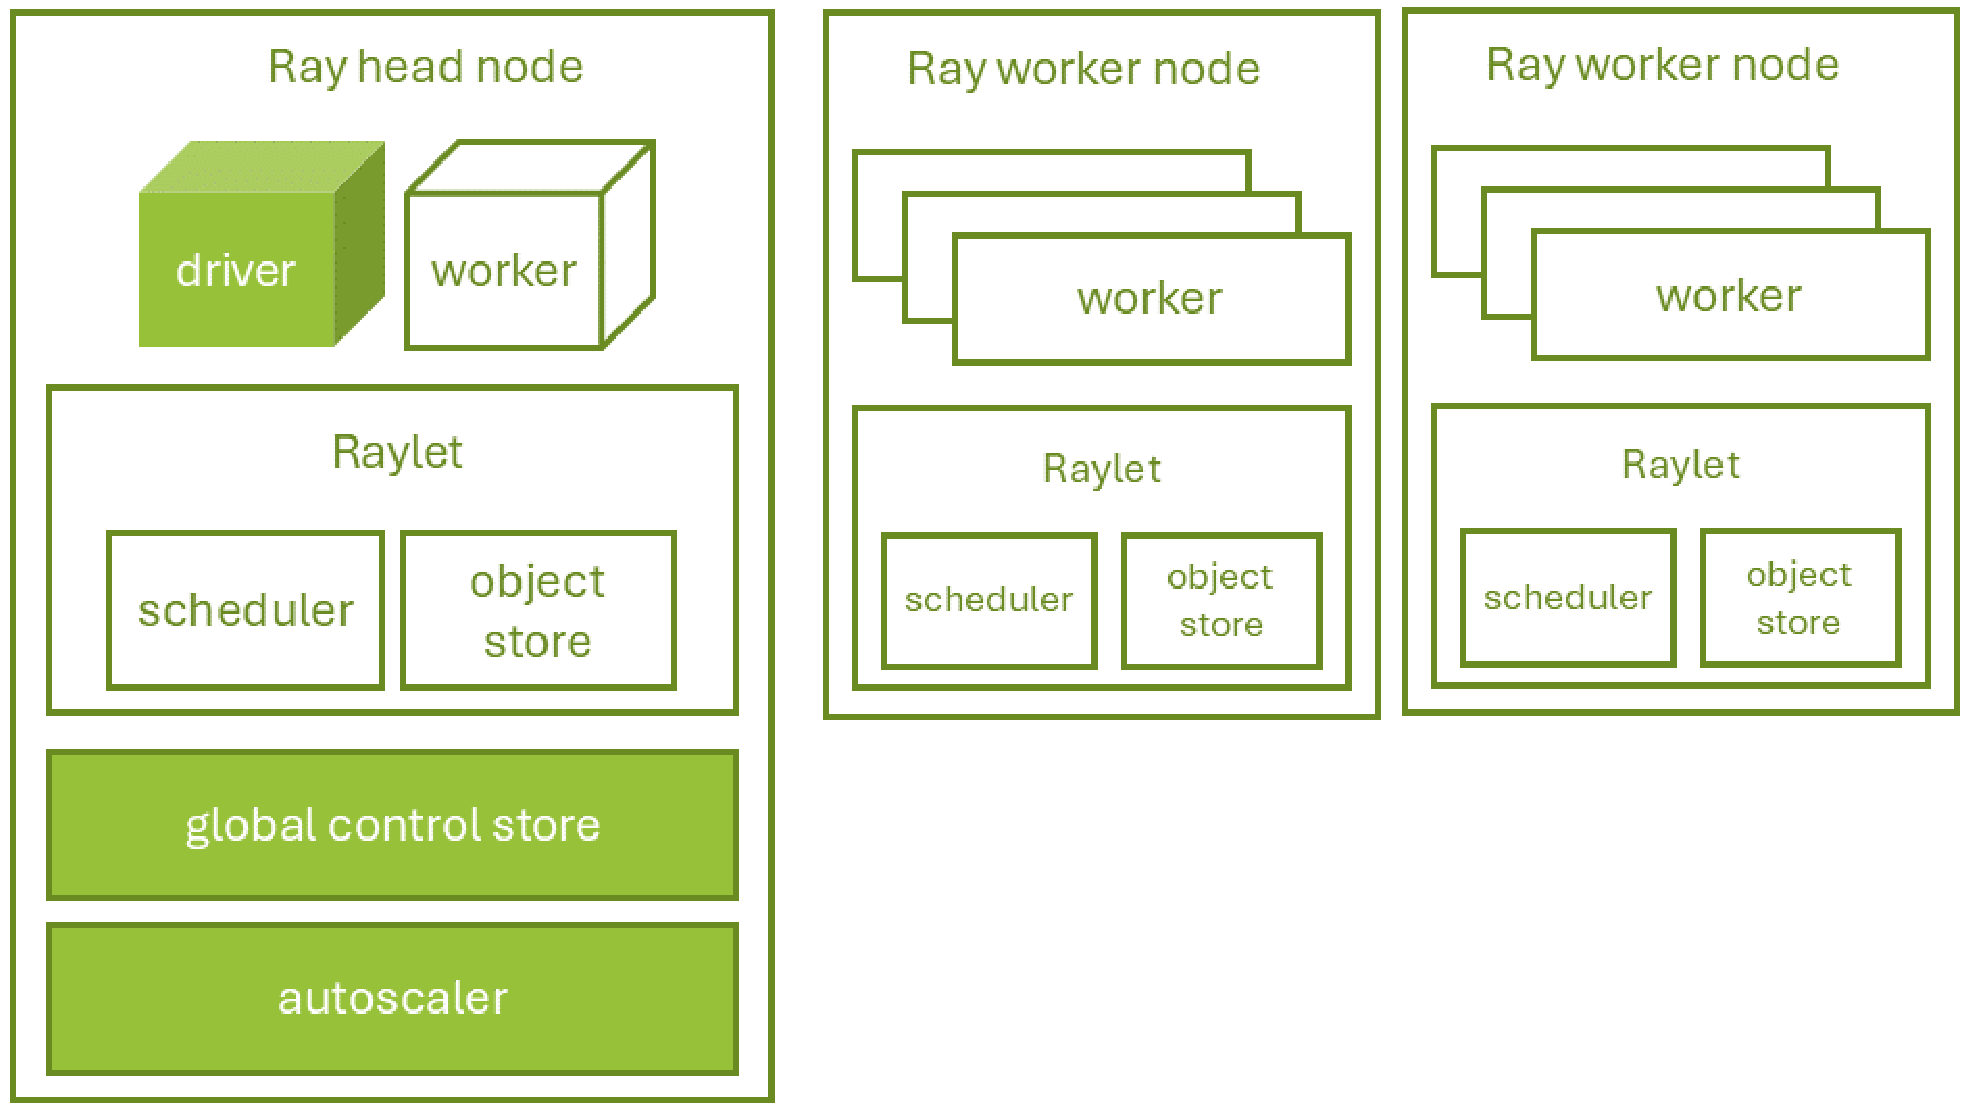
\includegraphics[width=1 \linewidth]{Thesis/Figures/Slide40.pdf}
\caption{\label{fig:Ray Cluster}Ray Cluster Architecture \cite{ray_doc}}
\end{figure}

\textbf{Head Node}

Each Ray cluster has a designated head node, which differs from worker nodes in that it manages cluster operations. The head node runs several essential singleton processes including the autoscaler, the global control store and the Ray driver processes responsible for executing Ray jobs. Although the head node can participate in task scheduling and actor management like any other worker node, it is generally recommended to avoid running tasks on it in large-scale clusters. This ensures optimal performance and resource allocation across the cluster. \cite{ray_doc}

\textbf{Worker Node}

Worker nodes are integral to running user code within Ray tasks and actors. Unlike the head node, worker nodes do not handle cluster management processes. Instead, they focus on distributed scheduling, storage and distribution of Ray objects within the cluster memory. The primary role of worker nodes is to execute tasks and actors, thus enabling efficient parallel processing across the cluster. \cite{ray_doc}

\textbf{Autoscaling}

The autoscaler, a process that operates on the head node or as a sidecar container in Kubernetes environments, manages the dynamic adjustment of worker nodes. When the resource demands of the Ray workload surpass the cluster’s current capacity, the autoscaler increases the number of worker nodes. Conversely, it will reduce the number of worker nodes when there is idle capacity. It is crucial to note that the autoscaler responds to task and actor resource requests rather than application metrics or physical resource utilization. \cite{ray_doc}

\clearpage

\textbf{Ray Jobs}

A Ray job refers to a single application consisting of Ray tasks, objects and actors derived from the same script. The worker running the Python script is termed the driver of the job. Ray jobs can be executed in two main ways as shown in \autoref{fig:Ray Job} by submitting the job using the Ray jobs API, which is the recommended approach, or by running the driver script directly on the Ray cluster for interactive development. The Ray jobs API guide provides additional details on these workflows. \cite{ray_doc}


\captionsetup{justification=centering}
\begin{figure}[h]
\centering
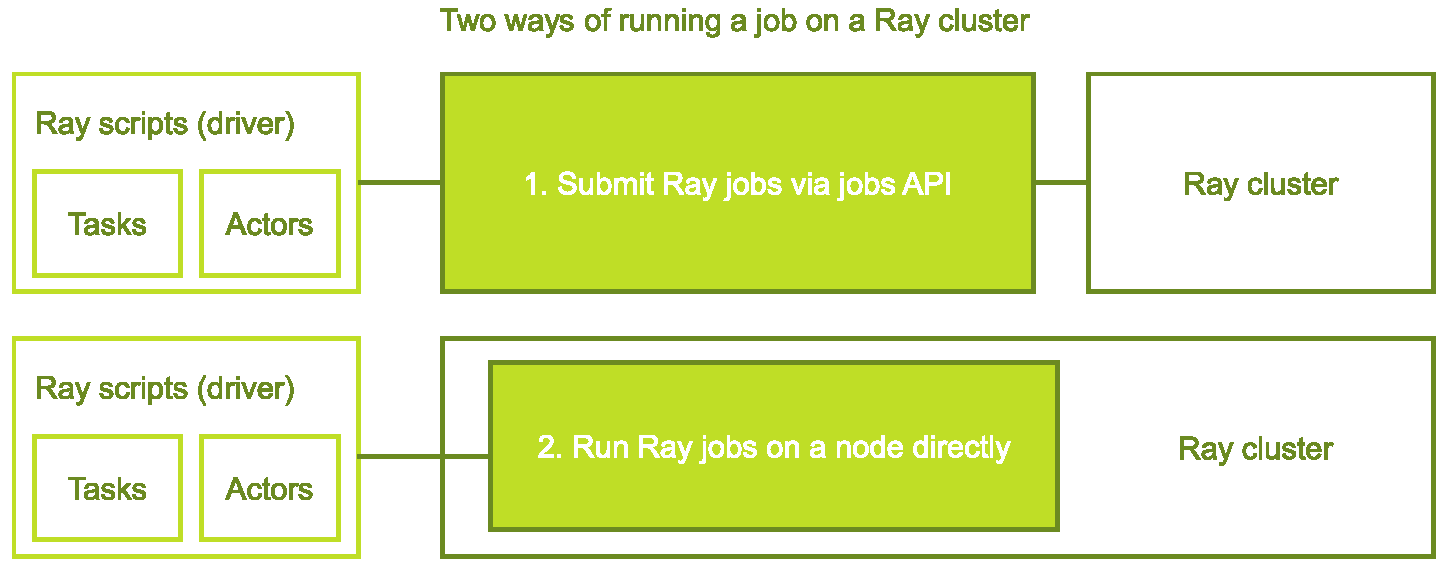
\includegraphics[width=1 \linewidth]{Thesis/Figures/Slide22.pdf}
\caption{\label{fig:Ray Job}Ray Job \cite{ray_doc}}
\end{figure}



\subsection{KubeRay Operator}

The KubeRay operator is a Kubernetes native operator designed to manage Ray clusters on Kubernetes efficiently. It simplifies the deployment, scaling and management of Ray clusters by leveraging Kubernetes robust orchestration capabilities. By using the KubeRay operator, developers can benefit from Kubernetes features such as automated rollouts, rollbacks, service discovery and resource management, which are seamlessly integrated into Ray architecture. This integration allows for enhanced scalability and reliability of distributed AI workloads running on Ray. The KubeRay operator defines custom resource definitions \abk{CRD}{Custom Resource Definitions} that represent the desired state of a Ray cluster. It ensuring that the cluster remains in optimal condition by continuously monitors the actual state of the cluster and reconciles it with the desired state. This includes managing Ray head and worker nodes shown in \autoref{fig:KubeRay Operator}, handling node failures and scaling the cluster based on workload demands. By automating these tasks the KubeRay operator reduces the operational burden on developers and enables them to focus more on developing AI models and less on infrastructure management.This integration of Ray with Kubernetes through the KubeRay operator provides a powerful solution for delivering and managing scalable AI applications in a cloud-native architecture. \cite{anyscale_blog, ray_doc}

\clearpage

\captionsetup{justification=centering}
\begin{figure}[h]
\centering
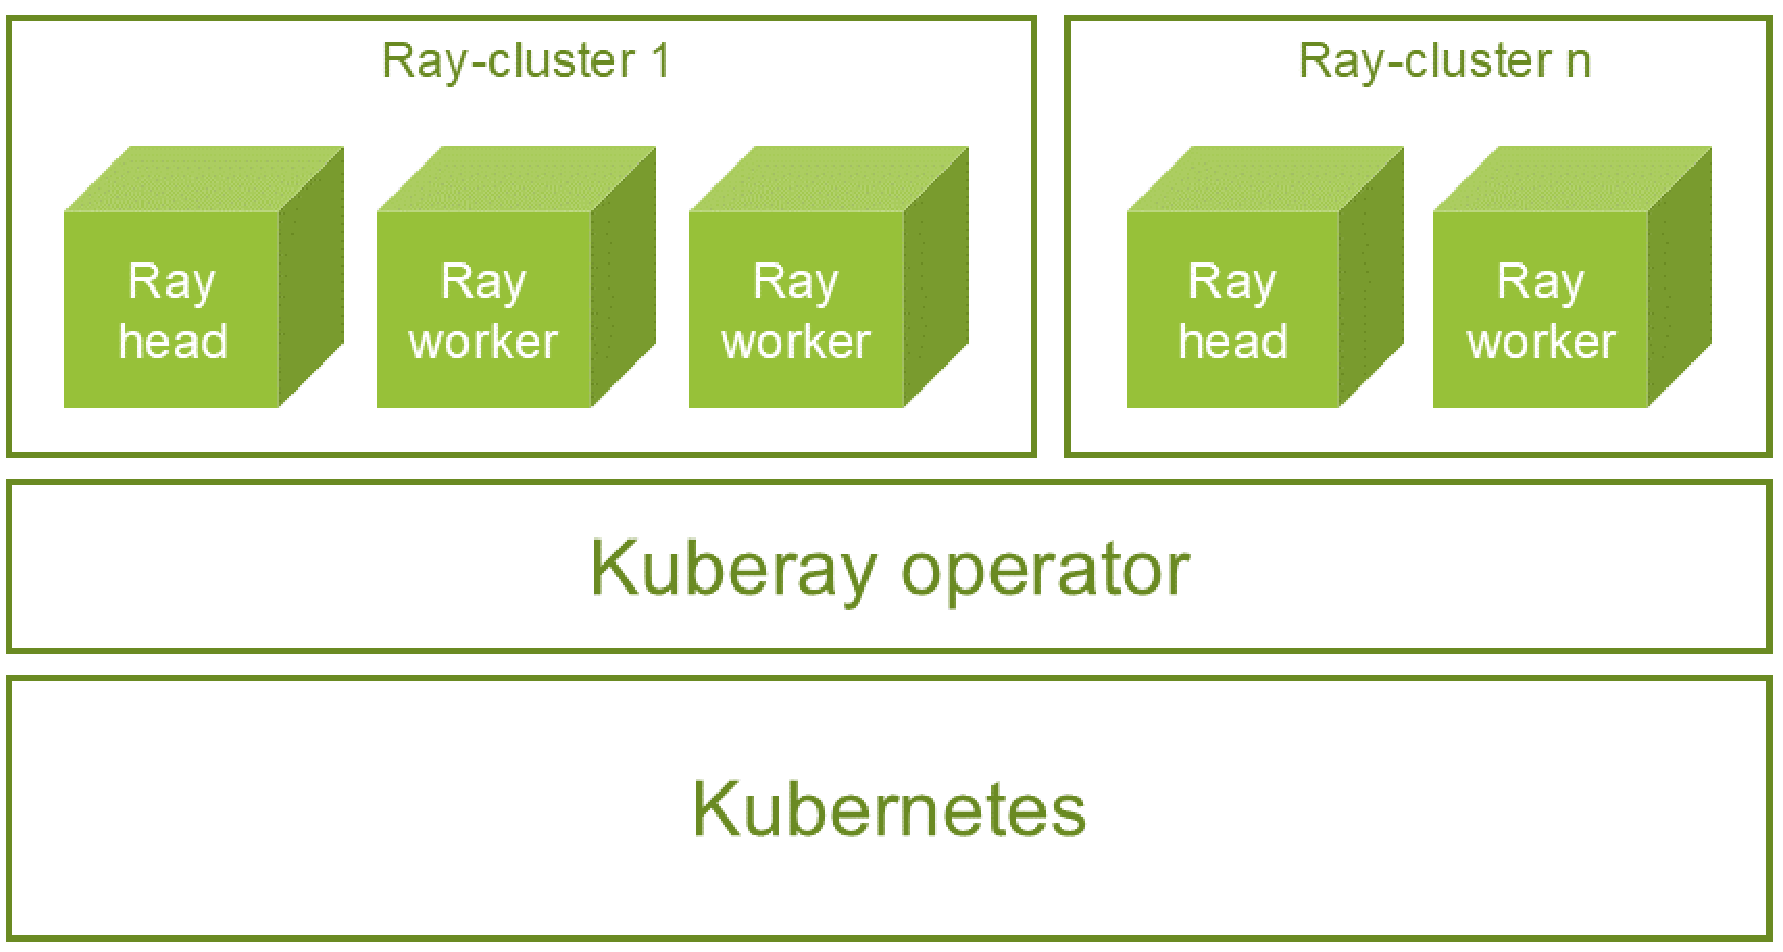
\includegraphics[width=1 \linewidth]{Thesis/Figures/Slide14.pdf}
\caption{\label{fig:KubeRay Operator}KubeRay Operator \cite{r34}}
\end{figure}

\subsection{Ray Core}

Ray core is the fundamental building block of the Ray ecosystem, it offers a distributed execution engine that support scalability and parallelism required for AI and ML workloads. The setup Ray core environment Helm charts or Kubernetes manifests is used, which outline the required configuration for Ray components. Configurations typically specify the cluster size, resource allocations and environment variables, ensuring that the Ray cluster can dynamically scale in response to workload demands. Ray core serves as the backbone for other Ray libraries, such as Ray tune, Ray train and Ray serve. It manages distributed task scheduling, state management and fault tolerance which are essential for the efficient execution of parallel computations. The integration of Ray core with Kubernetes through KubeRay allows for advanced features like autoscaling and resource management, ensuring that the cluster adapts to varying workloads while maintaining optimal performance. \cite{ray_doc}


\textbf{Ray Task}

Ray tasks are functions that can be executed remotely, allowing them to run concurrently across different nodes in the cluster. These tasks are defined using the \texttt{@Ray.remote} decorator and their execution is managed by distributed scheduler of Ray. The code snippet \autoref{listingsnippet:3} shows, a simple Ray task. This task will be executed on one of the available worker nodes and the result will be returned to the head node. \cite{ray_doc}


\listingsnippet{Ray Task Example \cite{ray_doc}}{

\vspace{0.3cm}

\hspace{0.25cm}\texttt{import ray}

%\vspace{0.1cm}

\hspace{0.25cm}\texttt{ray.init()}

%\vspace{0.1cm}

\hspace{0.25cm}\texttt{@ray.remote}

\vspace{0.3cm}

\hspace{0.25cm}\texttt{def mytask(x):}

\hspace{0.75cm}\texttt{return x + x}

\vspace{0.3cm}

\hspace{0.25cm}\texttt{result = ray.get(my-task.remote(4))}


\hspace{0.25cm}\texttt{print(result)  \# Output: 8}

\vspace{0.3cm}
}


\textbf{Ray Actor}

Ray actors extend the concept of Ray task by allowing stateful computations. An actor is essentially a Python class where each method invocation is treated as a remote task. Actors are particularly useful when managing state across tasks, as they maintain their state in-memory across multiple invocations. Code snippet \autoref{listingsnippet:4} shows the example how actors are used in scenarios where maintaining state consistency across distributed tasks is critical. \cite{ray_doc}

\listingsnippet{Ray Actor Example \cite{ray_doc}}{

\vspace{0.3cm}

\hspace{0.25cm}\texttt{@ray.remote}

\hspace{0.25cm}\texttt{class Counter:}

\vspace{0.3cm}

\hspace{0.75cm}\texttt{def init(self):}

\hspace{1.5cm}\texttt{self.count = 0}

\vspace{0.3cm}

\hspace{0.75cm}\texttt{def increment(self):}

\hspace{1.5cm}\texttt{self.count += 1}

\hspace{1.5cm}\texttt{return self.count}

\vspace{0.3cm}

\hspace{0.25cm}\texttt{counter = Counter.remote()}

\hspace{0.25cm}\texttt{print(ray.get(counter.increment.remote()))  \# Output: 1}

}


\textbf{Ray Core Methods}

Ray Core provides a number of methods that facilitate distributed computing. These methods simplify the process of parallelizing and distributing tasks across a cluster of machines. Key methods include

\begin{itemize}
    \item Ray.init()
    \item Ray.remote()
    \item Ray.get()
    \item Ray.put()
    \item Ray.shutdown()
\end{itemize}

The \texttt{Ray.init()} method initializes the Ray runtime and connects the Python program to the Ray cluster. It's the first step in setting up a Ray program and can be configured to connect to either a local Ray instance or a remote cluster. The \texttt{Ray.remote()} decorator is used to define Ray tasks or actors. By marking a Python function or class with \texttt{Ray.remote}, It automatically distributes the function execution or class instantiation across the cluster, allowing parallel computation. The \texttt{Ray.get()} method is used to retrieve results from Ray tasks or actor methods. As Ray executes tasks asynchronously, \texttt{Ray.get()} is used to block execution until the results are available to facilitate synchronization across the distributed system. The \texttt{Ray.put()} method allows large objects to be stored in the distributed object store so that they can be shared efficiently between tasks and actors without duplication, thus optimising memory usage in the cluster. Finally, the \texttt{Ray.shutdown()} method neatly shuts down the Ray runtime, ensuring that all tasks are completed and resources are properly freed, which is critical to maintain cluster stability. Ray core methods enable seamless interaction with the distributed system, allowing developers to focus on their application logic without worrying about the complexities of distributed computing. These methods, combined with the orchestration capabilities of Kubernetes, provide a powerful platform for scaling AI and ML workloads. \cite{ray_doc}


\textbf{Sequential Implementation}

In a sequential implementation of Ray, tasks or functions are executed one at a time, in a single thread or process, as shown in \autoref{fig:sequential}. This traditional approach works well for simpler workloads or where the overhead of parallelism outweighs the benefits. However, it limits the ability to take full advantage of multi-core CPUs and distributed systems. In this mode, Ray behaves like a normal Python program, where each function is executed in the order it's called and the system waits for the current task to finish before moving on to the next. This limits scalability, but can be easier to debug and manage for small tasks. \cite{ray_doc}



\begin{figure}[h]
\centering
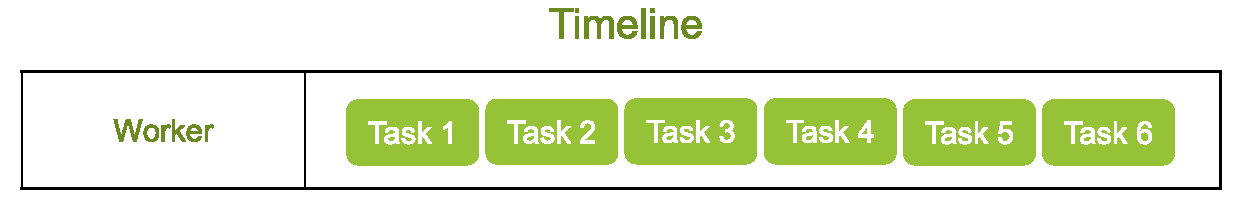
\includegraphics[width=1 \linewidth]{Thesis/Figures/Slide68.pdf}
\caption{\label{fig:sequential}Sequential Implementation of Tasks \cite{ray_doc}}
\end{figure}



\textbf{Parallel Implementation}

Parallel implementation of Ray, uses all available resources to train models in parallel, maximizing computational efficiency. Ray automatically detects the number of cores on your machine, or the available resources in a cluster and dynamically distributes each task across them as shown in \autoref{fig:parallel}. Instead of processing tasks sequentially, Ray introduces a scheduler that manages incoming requests, assigns them to nodes and monitors resource availability to ensure optimal use. This parallel execution model accelerates processing by using multiple cores or machines simultaneously, resulting in significant performance improvements, especially for resource intensive tasks such as ML model training. \cite{ray_doc}

\clearpage

\begin{figure}[h]
\centering
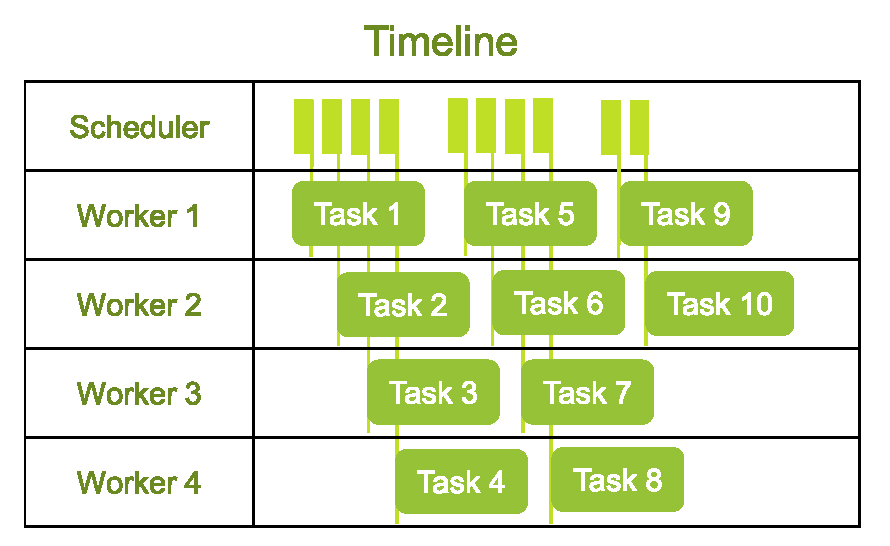
\includegraphics[width=1 \linewidth]{Thesis/Figures/Slide69.pdf}
\caption{\label{fig:parallel}Parallel Implementation of Tasks \cite{ray_doc}}
\end{figure}

\subsection{Ray Data}

Ray data is a key component of the Ray ecosystem, designed to handle large-scale data processing tasks in a distributed manner across multiple nodes within a cluster. It facilitates the seamless distribution of datasets, enabling parallel processing and transformation of data, which is essential for scaling ML and data intensive applications. By integrating with other Ray modules, Ray Data enables efficient handling of diverse workloads such as data loading, pre processing and transformation, while ensuring that operations are distributed to maximize resource utilization and minimize processing time. Ray Data emerges as the most suitable solution for scalable and high performance data processing. Ray Data provide the distributed processing capabilities to efficiently manage the dataset across the Ray cluster. Instead of relying on traditional single node data handling, the dataset was distributed across multiple nodes, ensuring that data loading and processing tasks were executed concurrently. This approach allows to scale operation with less processing time by distributing tasks across the cluster and achieve high level of parallelism as shown in \autoref{fig:Ray Data}, which significantly improved the throughput and responsiveness of our system. This implementation demonstrated the effectiveness of Ray Data in managing large-scale data processing workflows within a distributed environment, aligning with the goals of scalability and efficiency. \cite{ray_doc}

\clearpage

\begin{figure}[h]
\centering
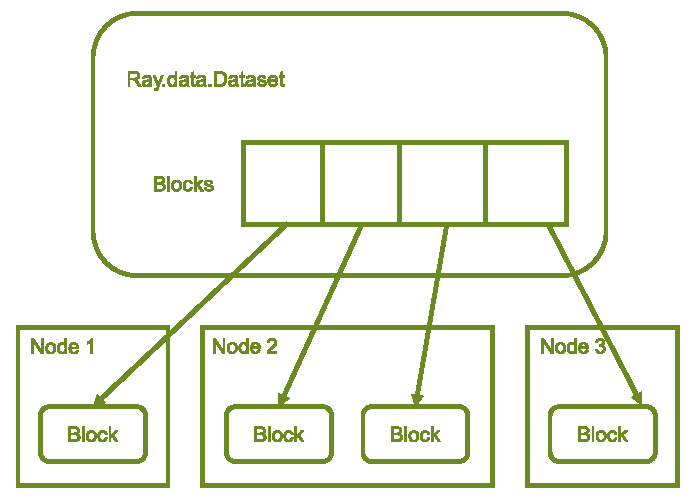
\includegraphics[width=0.9 \linewidth]{Thesis/Figures/Slide52.pdf}
\caption{\label{fig:Ray Data}Ray Data Overview \cite{anyscale_blog}}
\end{figure}



\subsection{Ray Train}

Ray train is a core component of the Ray ecosystem that enables distributed training of model across multiple nodes. It is designed to handle large ML and DL workloads by distributing tasks in parallel to speed up the training process. Ray train integrates easily with other ML frameworks and provides built-in fault tolerance ensuring continues training even if some nodes fail. This capability is particularly useful when working with large datasets that require high computational resources. By using Ray train ML engineers can optimise their training workflows, reducing required time and efficiently scaling operations within a Kubernetes environment. The training process in Ray is organized around several components, such as training function, worker, scaling configuration and trainer. The training function consist of the core logic of model training including loading dataset, defining model and performing training iterations. The function is distributed across multiple nodes by Ray train, allowing parallel processing. By assigning each worker a separate process to perform the training function. The workers are distributed across the cluster, allowing the training logic to be executed concurrently. The distribution of workers allows efficient use of computational resources, whether CPUs or GPUs. Scaling configurations specify the number of workers and the computing resources allocated to each worker. This configuration is critical for optimising resource usage and ensuring that the training workload is appropriately balanced across the cluster. The trainer class then brings together the training function, the workers and the scaling configuration and orchestrates the execution of the distributed training job, managing the distribution of data and synchronization of results across the workers. Ray train conduct large-scale distributed training effectively also shown in \autoref{fig:Ray Train}. The scalability and fault tolerance provided by Ray train were essential in managing complex training tasks within the Kubernetes environment, ensuring high performance and reliability. \cite{ray_doc}

\begin{figure}[h]
\centering
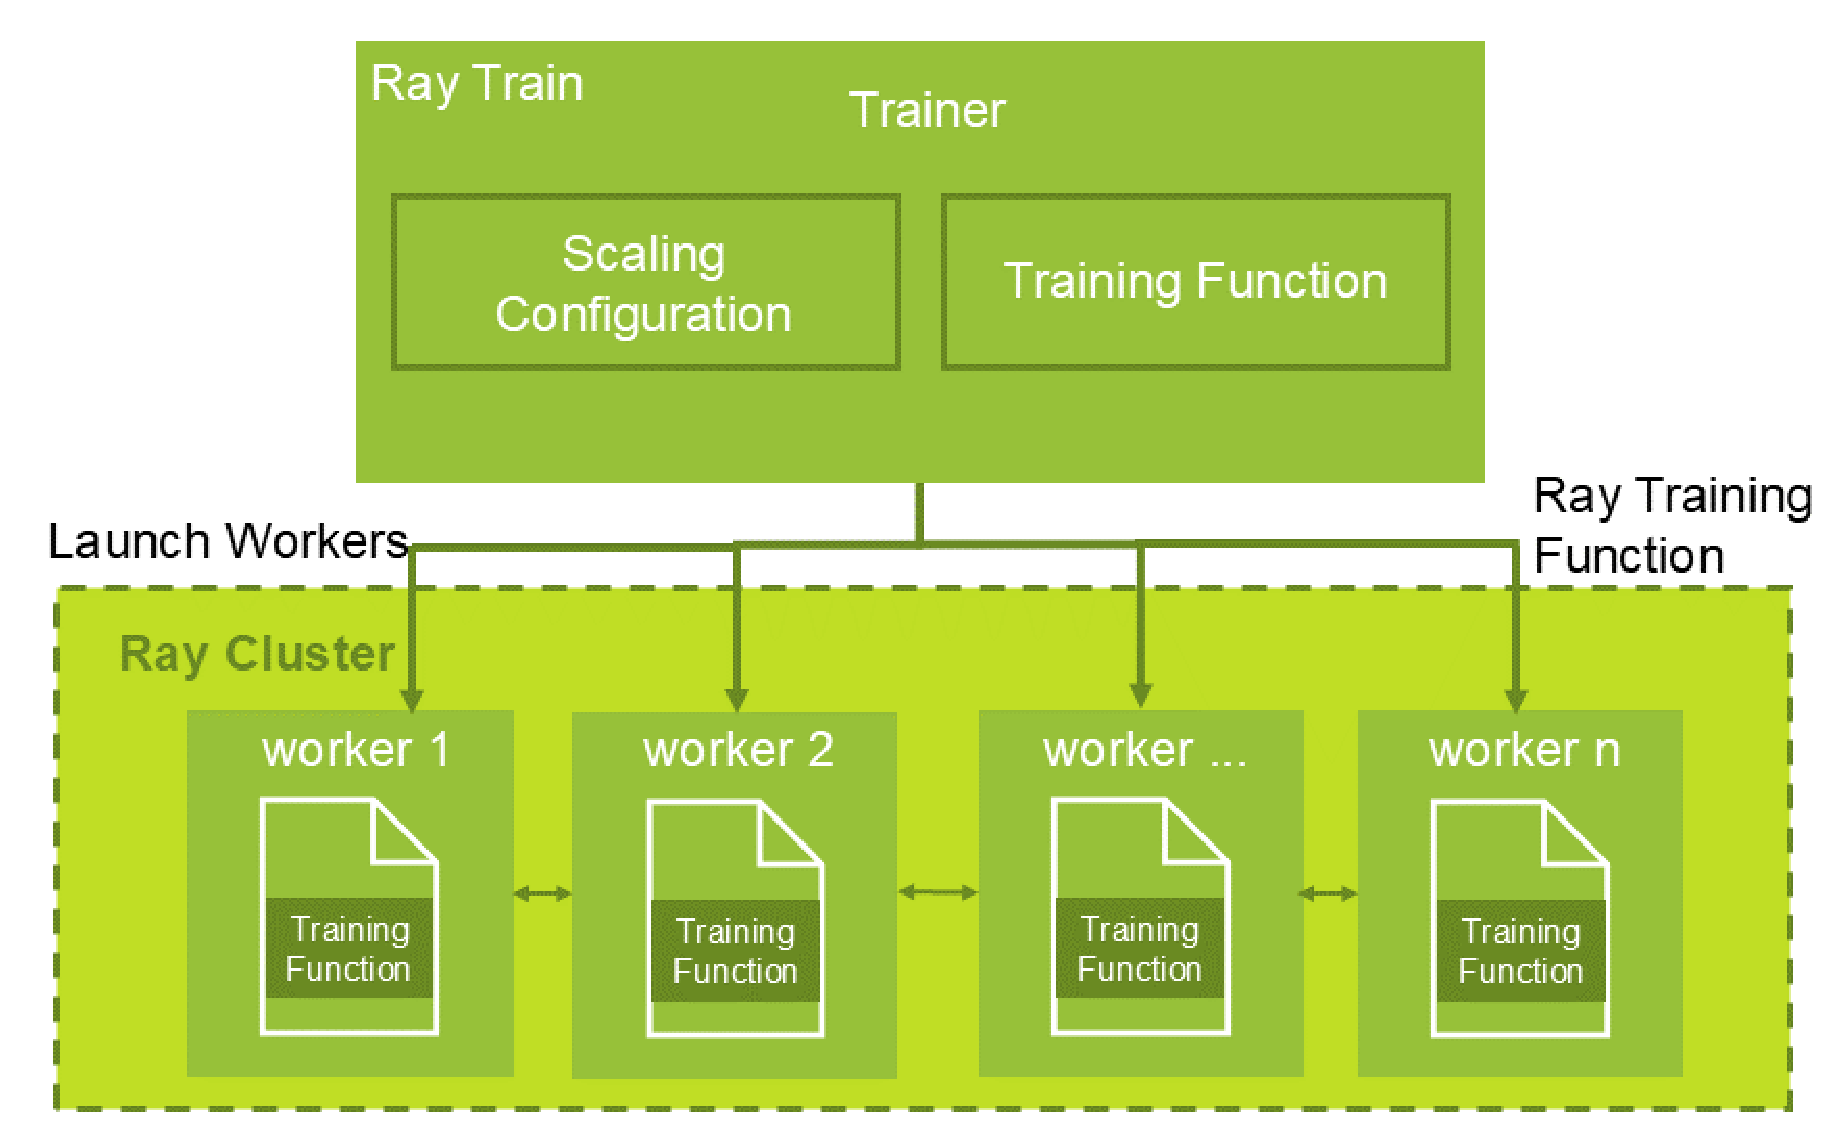
\includegraphics[width=1 \linewidth]{Thesis/Figures/Slide53.pdf}
\caption{\label{fig:Ray Train}Ray Train Overview \cite{ray_doc}}
\end{figure}


\subsection{Ray Tune}

Ray tune is a powerful optimization library that allows efficient exploration of hyperparameter spaces to find the best model configurations. It provides algorithms such as Population Based Training  and HyperBand to optimize and accelerate the tuning process.  Ray tune handles hyperparameter optimization by defining a search space for critical hyperparameters such as the number of estimators and the maximum depth of trees. Using this search space Ray tune can explore different combinations of these hyperparameters. Ray tune integration into the Ray ecosystem facilitates the distributed execution of hyperparameter optimization tasks. By utilizing the computational resources of Ray cluster, distributed tuning of workload across multiple nodes are possible see \autoref{fig:Ray Tune}, which significantly accelerated the optimization process. This distributed approach ensures that hyperparameter tuning is efficient and scalable, making it suitable for large-scale ML tasks. Ray tune also provides built-in support for logging and tracking the results of each trial. \cite{ray_doc}


\clearpage

\begin{figure}[h]
\centering
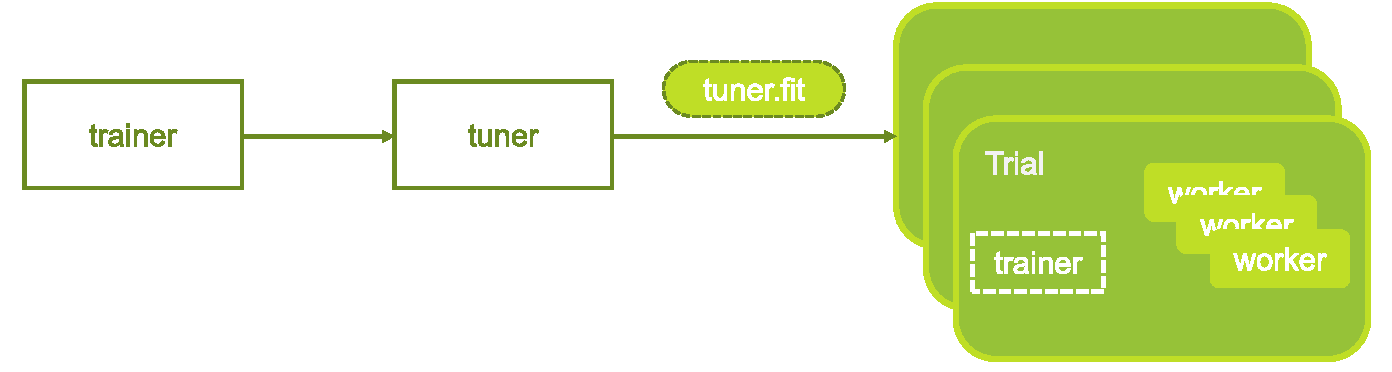
\includegraphics[width=1 \linewidth]{Thesis/Figures/Slide55.pdf}
\caption{\label{fig:Ray Tune}Ray Tune Overview \cite{ray_doc}}
\end{figure}



\subsection{Autoscaling with Ray}

Autoscaling of resources using Ray involves sequence of steps to achieve efficient resource utilization and performance of ML and DL workloads. First, Ray cluster must be configured to dynamically adjust the number of worker nodes based on the workload requirements. This is achieved through Ray autoscaler by defining the minimum and maximum number of nodes in a configuration file. Once autoscaler is configured, its start monitoring the resource usage and workload demands and automatically adds or remove worker nodes as needed to meet the workload demand. This dynamic scaling capability helps in optimizing resource allocation, reducing costs and maintaining high performance under varying workloads as shown in \autoref{fig:Autoscaling with Ray}. \cite{moritz}

Performance optimization techniques are crucial when enabling autoscaling with Ray. Key strategies of optimizing performance includes monitoring system metrics to identify bottlenecks, optimizing the configuration of worker nodes and fine tuning the scheduling policies to improve resource utilization. Additionally, leveraging Ray built-in libraries, such as tune for hyperparameter optimization and reinforcement learning libraries \abk{RLlib}{Reinforcement Learning Library}, can further enhance the efficiency and effectiveness of AI models. Developers can ensure that the system operates at peak, by continuously analyzing and adjusting the resource allocation, which provides a robust and scalable solution for deploying AI models in production environments. \cite{r52}

\makeatletter
\setlength{\@fptop}{0pt}
\makeatother


\begin{figure}[h]
\centering
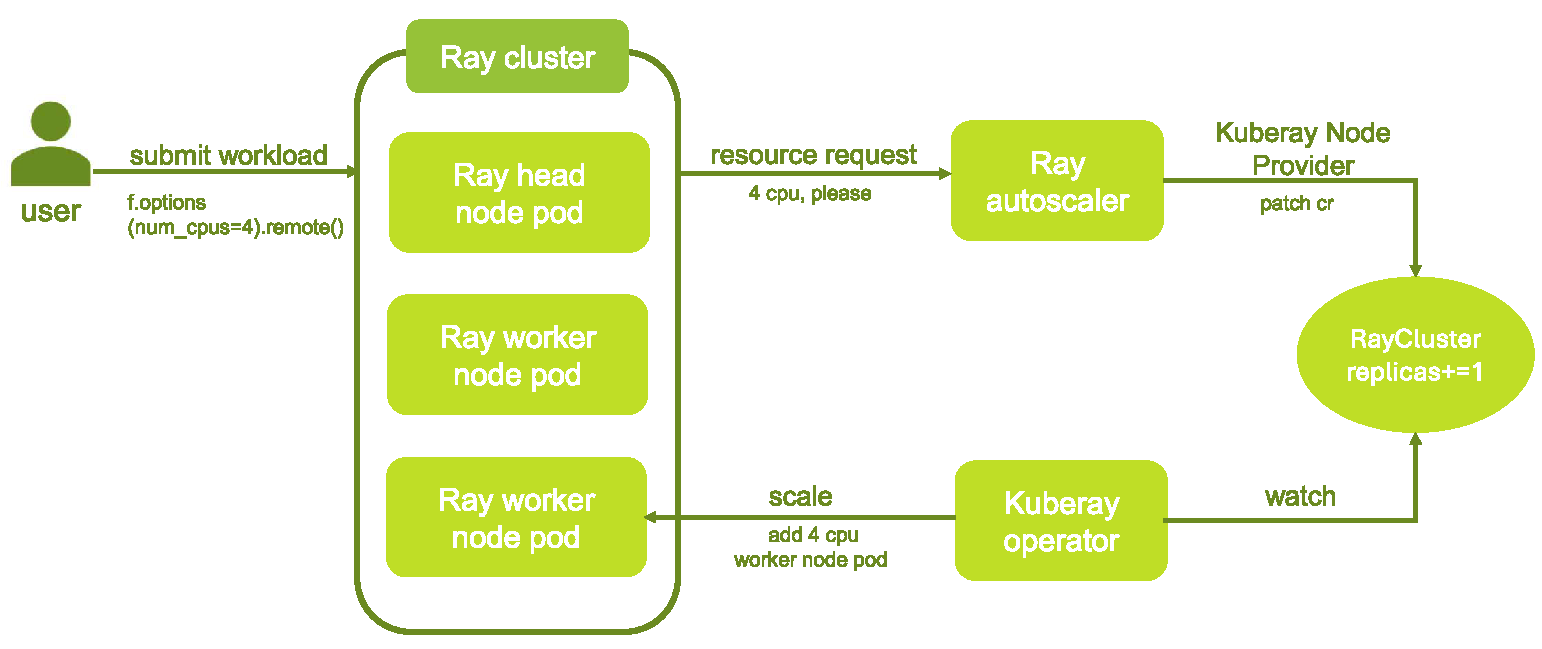
\includegraphics[width=1 \linewidth]{Thesis/Figures/Slide13.pdf}
\caption{\label{fig:Autoscaling with Ray}Autoscaling with Ray \cite{ray_doc}}
\end{figure}

  
            \chapter{Methodology}

A methodology for achieving security, scalability, and resource distribution in a cloud-native architecture is described in this chapter. The approach integrate different architectures to address specific research objectives and requirements. The primary objective of this research is the development of an architecture that provide secure, scalable and distributed computing platform. To achieve this objective, a combination of cloud-native technologies and tools are used, particularly in the context of AI model deployment.

\section{Authentication}

In a cloud-native architectures, authentication is the foundation for securing access to resources. Authentication provides protection of shared information from unauthorized access. It is essential for maintaining data security. Authentication methods are designed in a way that can verify the identity of users and confirm that they are who they claim to be and determine whether they are authorized to access sensitive information. In a cloud-native architectures, where multiple services and applications interact with each other, it become crucial to provide authentication mechanism to streamline access and maintain security. By implementing a secure SSO mechanism using authentication protocols, we can effectively authenticate users and enhance overall security. \cite{babaeizadeh2015authentication}

\subsection{Single Sign-On}

SSO is a cloud-native identity and access management solution in cloud-native architecture that enhance the security of the application and or user experience by centralizing the authentication system. SSO allows users to log in with a single set of credentials and then use many secure resources without having to log in again and also helps to reduce the number of passwords that users need to remember to access different applications, making it much more efficient and secure. SSO helps reduce the number of accounts, the administrative burden of managing user privileges and the likelihood of privilege violations. Implementing SSO with OIDC and OAuth helps to authenticate users and improve security by combining access management into a single, manageable framework. \cite{babaeizadeh2015authentication}

\subsection{Authentication Protocol}

Authentication protocols are essential for implementing SSO, as they provide standardised methods for managing user authentication and authorization across different applications. Commonly used protocols include OAuth2, SAML and OpenID, each of which plays an important role in improving security and streamlining access. OAuth is an open authorization protocol that enables secure access to resources by issuing tokens rather than using traditional username and password methods. SAML facilitate communication between identity providers and service providers with regards to SSO using different authentication methods, it is one of the core components of cross domain SSO implementation frameworks.. OpenID, on the other hand, allows users to authenticate without relying on a central server and uses identifiers, trusted parties and providers to manage user authentication and verification processes. The using these protocols, the aim is to create an SSO mechanism that simplifies user access and improves overall security in our cloud-native architecture. \cite{waluyo2022comparative}

\section{Authorization and Access Control}

Once a request has been authenticated, it moves on to the authorization phase, which is a critical part of securing Kubernetes clusters, ensuring that only authenticated users and services with the appropriate permissions can interact with cluster resources. This involves verifying whether a user or service is allowed to perform a specific action on a specific resource. This process is used to hold security and prevent intrusion since it adheres to certain policies that determine potential security risks and actions to avoid those risks, by protecting potentially vulnerable areas in cloud-native architectures. \cite{zahoor2023formal}

Access control is the mechanism used to grant permissions within the cluster. In Kubernetes, The RBAC system allows to control access to resources in a more granular manner through building different levels of permissions and policies. This system regulates the actions that users and service accounts are allowed to perform, ensuring that only authorized entities can access and interact with critical resources. To enhance the security of our Kubernetes cluster in a cloud-native architectures, we will implement RBAC as a fundamental component of our access control strategy. \cite{mustyala2021advanced}

\section{Distributed Computing Framework}

Distributed computing frameworks are critical components of cloud-native architectures that enable efficient processing of large amounts of data on clusters or in the cloud. Their main purpose is to distribute computing work across multiple computers, reducing the load and potential risks of concentrating computing on a single computer and providing high scalability, reliability, manageability and flexibility. As the size and complexity of AI models grow faster than the computing power of clusters, traditional distributed computing frameworks based on the MapReduce model are insufficient to support AI tasks. These tasks often involve running complex analytical algorithms on large-scale AI models with billions of parameters. However, existing frameworks face key challenges such as computational inefficiency, limited scalability due to memory constraints, and limited algorithmic capabilities because many sequential algorithms cannot be implemented within the MapReduce programming model. Therefore, new distributed computing frameworks are needed to address these challenges. This research utilized a flexible distributed computing framework with the potential to overcome the challenges of AI model analysis and provide autoscaling to ensure resource scalability. \cite{sun2023survey, chen2023advance}

\subsection{Optimization of AI Models}

Optimising AI models at scale requires the use of distributed computing frameworks due to the significant complexity and size of modern machine learning problems. As data volumes and model complexity continue to escalate, with datasets ranging from 1TB to 1PB and models containing between $10^9$ and $10^{12}$ parameters, it becomes impractical for a single machine to perform the required computations efficiently. Distributed optimization frameworks are essential to deal with these challenges on a large-scale. In a distributed setup, both data and computational workloads are distributed across multiple worker nodes. These nodes collaborate by frequently accessing and updating shared parameters, which can be represented as dense or sparse vectors and matrices. The distributed framework handles the asynchronous data communication between nodes for the purpose of maintaining consistency of the global parameters across all workers. This approach supports various consistency models enabling further control of data consistency and synchronization. By using distributed computing, optimization can solve fundamental problems of large and complex ML and DL models and improve the training process of large-scale AI models. \cite{li2014scaling}

\subsection{Scalability of Resources}


Scalability is an apt feature in distributed computing frameworks like Kubernetes cluster that is used for handling dynamic workloads to achieve efficient resource utilization. The resource scaling is
normally done with regards to the number of replicas of any workload or the number of replicas modified with respect to the ratio between the current metric value as well as the target metric value. The formula used to calculate for the number of replicas needed is

\[
\text{desiredReplicas} = \left\lceil \text{currentReplicas} \times \left( \frac{\text{currentMetricValue}}{\text{desiredMetricValue}} \right) \right\rceil
\]


This equation calculate and adjust with the number of replicas depending on workload such as when the current value is two times the desired metric, the system will set the number of replicas equal to multiple of two to the current metric value. On the other hand, if the current load is cuts down to half of its required value, the number of replicas is also halved. The scaling action is isolated if the current and the corresponding desired value is close enough to a small and adjustable tolerance thus avoiding unnecessary scaling actions, even if the values are not optimal. It is one of the scalability techniques that control the computing resources considering the changes of workload, it can provide dynamic allocation of resources which in result helps to control the performance and prevent waste of resources. Due to their ability to scale up or down, and distribute the work, distributed frameworks are more reliable and adaptable to the changing conditions and to achieve best performance by the use of dynamic computing resources. \cite{Kubernetes_doc}


\clearpage



\autoref{fig:Secure and Scalable} below illustrates the secure, scalable and distributed computing architecture using
distributed computing framework to implement authentication and authorization to achieve a secure, scalable, and distributed computing architecture that is capable of deploying the AI model.

\begin{figure}[h]
\centering
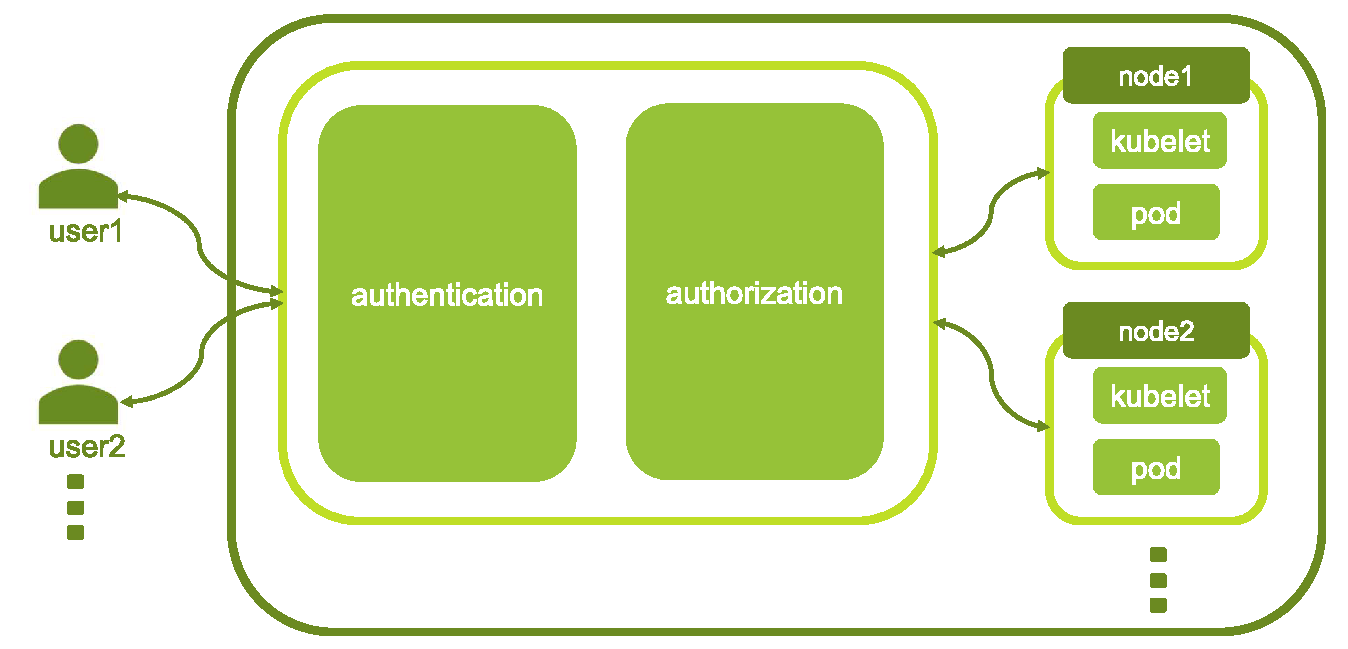
\includegraphics[width=1 \linewidth]{Thesis/Figures/Slide47.pdf}
\caption{\label{fig:Secure and Scalable}Secure and Scalable Architectures}
\end{figure}


            
            \chapter{Implementation}


The research implements security, scalability and resource distribution within a cloud-native architecture to support AI workloads. It uses key technologies like Keycloak for authentication, Kubernetes RBAC for authorization and Ray for scalability and distributed computation. This implementation chapter is focus on three key elements that are essential to achieve secure, scalable and resilient cloud-native architecture.

\textbf{Implementation of Authentication with Keycloak for ArgoCD} 


Authentication is the basic requirement for securing access to resources. In this research, Keycloak which is an open source IAM solution, is introduced and configured with ArgoCD, which is a declarative GitOps tool for Kubernetes, to handle authentication using SSO. This integration ensures that only the authorized users can access and perform user task on the deployment processes. \cite{redhat_docs}

\textbf{Implementation of Authorization with Role-Based Access Control} 

Following the process of authentication the next main step is that of authorization. In Kubernetes RBAC is implemented to regulate user actions within the cluster. RBAC ensures that users have only the necessary permissions, by defining roles and binding them to users, thereby enhancing the security and governance of the cluster. \cite{Kubernetes_doc}

\textbf{Deploying Scalable Architecture and Enabling Autoscaling with Ray} 

For resource intensive tasks scalability is a crucial part of cloud-native environments, especially when dealing with AI and ML workloads. Ray is deployed on the Kubernetes cluster to manage AI model training and scalability of resources. The architecture is designed to scale horizontally, with autoscaling using Kubernetes HPA and Ray distributed capabilities. This makes the architecture effective in using resources optimally and addressing challenges in changing workloads. \cite{moritz, Kubernetes_doc}

In this manner, this implementation provides a comprehensive, secure and scalable cloud-native architecture suitable for complex AI, ML and distributed applications.

\section{Tools and Technologies}

To implementing security and scalability in a distributed computing architecture several key tools and technologies are required, each chosen for their specific capabilities and alignment with the research objectives. It uses key technologies such as Keycloak and Kubernetes RBAC for security and Ray for resource distribution. Kubernetes was used to orchestrate and manage containerized applications and allow to scale the system dynamically based on workload demands \cite{Kubernetes_doc}. It provided the necessary infrastructure to deploy, scale and manage containerized services in a reliable and automated manner  \cite{Kubernetes_doc}. The autoscaling capabilities of Kubernetes are particularly valuable in maintaining system performance under varying workloads \cite{Kubernetes_doc}. For authentication, Keycloak was integrated into the system to manage user identities and secure access to the platform. Keycloak's robust authentication capabilities, including support for SSO and multiple authentication protocols, made it a suitable choice for securely and efficiently managing user access. \cite{keycloak_doc}. To manage and enforce permissions within the system, RBAC was implemented as the primary authorization mechanism  \cite{Kubernetes_doc}. RBAC enabled granular access to resources by defining roles and permissions, ensuring that only authorised users could perform specific actions within the infrastructure \cite{Kubernetes_doc}. Ray was chosen to manage and distribute tasks across multiple nodes. Its ability to handle large computations by distributing tasks across a cluster made it an ideal choice for managing AI workloads \cite{moritz}. Ray also supports for training and tuning of large-scale AI models by distributing processes across available resources, significantly increasing computational efficiency \cite{moritz}.


\subsection{Rationale for their Selection}

Each tool has been selected in order to provide a cloud-native architecture that will be as safe as possible and at the same time as scalable as possible. This section outlines the key factors that influenced the choice of technologies based on their contribution to overall system performance and security. Keycloak was chosen to provide SSO and its comprehensive authentication features which include support for openID, OAuth and SAML authentication protocols \cite{keycloak_doc}.  RBAC was implemented to provide a fine-grained authorization model, enabling the system to enforce strict access controls system to maintain security across different layers of the infrastructure \cite{Kubernetes_doc}. Ray's compatibility with Kubernetes enabled seamless deployment and scaling of computational tasks, while Keycloak and RBAC provided a cohesive security framework that integrated well with other components \cite{ray_doc, keycloak_doc}. When considering scalability and efficiency, Ray was chosen for its proven ability to manage distributed computation, particularly in environments where large-scale AI tasks are common and Kubernetes was chosen for its mature and robust container orchestration capabilities, allowing the system to scale both horizontally and vertically to meet compute demands. Together these tools ensured that system could handle significant workloads with minimal manual intervention. \cite{ray_doc}


\subsection{Setup and Configuration Details}

This section provides information on the tools used for security, scalability and resource distribution. Container orchestration is the fundamental platform for developing large-scale distributed applications with a high level of security and access control. 
In first step, Kubernetes is configured to manage the lifecycle of containerised applications including the deployment and scaling of Ray processes which includes setting up clusters and defining resource allocations \cite{Kubernetes_doc}. Keycloak was then configured to manage authentication across the system. The integration process involved setting up Keycloak as an identity provider and configuring it to work with the existing services \cite{keycloak_doc}. Once the setup and configuration of Kubernetes and Keycloak was complete the RBAC system was configured by defining roles and permissions tailored to the needs of the system. This involved creating policies that determined which users could access specific resources and perform specific actions ensuring that security policies were consistently enforced across the infrastructure \cite{Kubernetes_doc}. Finally, Ray was set up to operate within a Kubernetes managed cluster with nodes configured to handle distributed computational tasks. The setup involved defining the cluster architecture, specifying resource limits and configuring the framework to efficiently manage the distribution and execution of tasks. \cite{ray_doc}

\clearpage

\section{Implementation of Authentication Using Keycloak for ArgoCD}

Integrating Keycloak with ArgoCD is essential for establishing a secure and centralized authentication mechanism that aligns with modern security practices \cite{argocd_docs}. ArgoCD, a declarative GitOps continuous delivery tool for Kubernetes \cite{argocd_docs}, requires a robust and SSO authentication solution to control access to its web interface \cite{keycloak_doc}. This integration allows us to manage authentication in a centralized manner, enforcing consistent security policies across their deployment workflows \cite{redhat_docs}. Integrating Keycloak with ArgoCD provides several advantages. First, it centralizes authentication, allowing administrators to manage user credentials and access policies in one place, reducing complexity and improving security \cite{redhat_docs}. Second, Keycloak supports industry standard protocols such as OAuth2, OIDC and SAML, which provide a secure and standardized way to handle authentication and authorization \cite{oauth_oidc_intro}. This integration not only enhances the security of ArgoCD but also ensures that only authenticated and authorized users can access critical deployment pipelines, thereby protecting the integrity of the Kubernetes clusters \cite{Kubernetes_doc}.

\subsection{Selection of Authentication Protocol}

OAuth 2.0, OIDC and SAML are authentication protocols supported by keycloak. OIDC is an extension of OAuth 2.0 where OAuth 2.0 is a framework for building authorization protocols but it is incomplete. OIDC on the other hand is a complete authentication and authorization protocol that uses the JWT standards. The JWT standards define a JSON format for identity tokens and methods for digitally signing and encrypting data in a compact and web friendly way. Finally, SAML 2.0 is a specification similar to OIDC but more mature. It is derived from Web services messaging specifications, so it is generally more verbose than OIDC. SAML 2.0 protocol exchanges XML documents between authentication servers and applications. XML signatures and encryption are used to verify requests and responses. In this research we implemented OIDC, which is recommended by Keycloak as it is specifically designed to work with the web and is suitable for HTML5 or JavaScript applications as it is easier to implement on the client side than SAML. OIDC provides a browser based authentication code flow, in which when a user attempts to access ArgoCD, they are redirected to Keycloak where they must authenticate. Upon successful authentication, Keycloak issues an ID token and an access token based on the on the OIDC protocol, which ArgoCD then uses to grant access to its resources, as shown in \autoref{fig:Keycloak OIDC}. This setup not only secures the authentication process but also provides SSO capabilities, allowing users to access multiple services, including ArgoCD, with a single set of credentials. Integration of Keycloak with ArgoCD using OIDC ensures
a secure and centralised authentication process. Using this approach provides a robust solution for managing access to ArgoCD according to identity management best practices while increasing the security of the Kubernetes environment \cite{argocd_docs, oauth_oidc_2023}. \cite{keycloak_doc}



\clearpage

\begin{figure}[h]
\centering
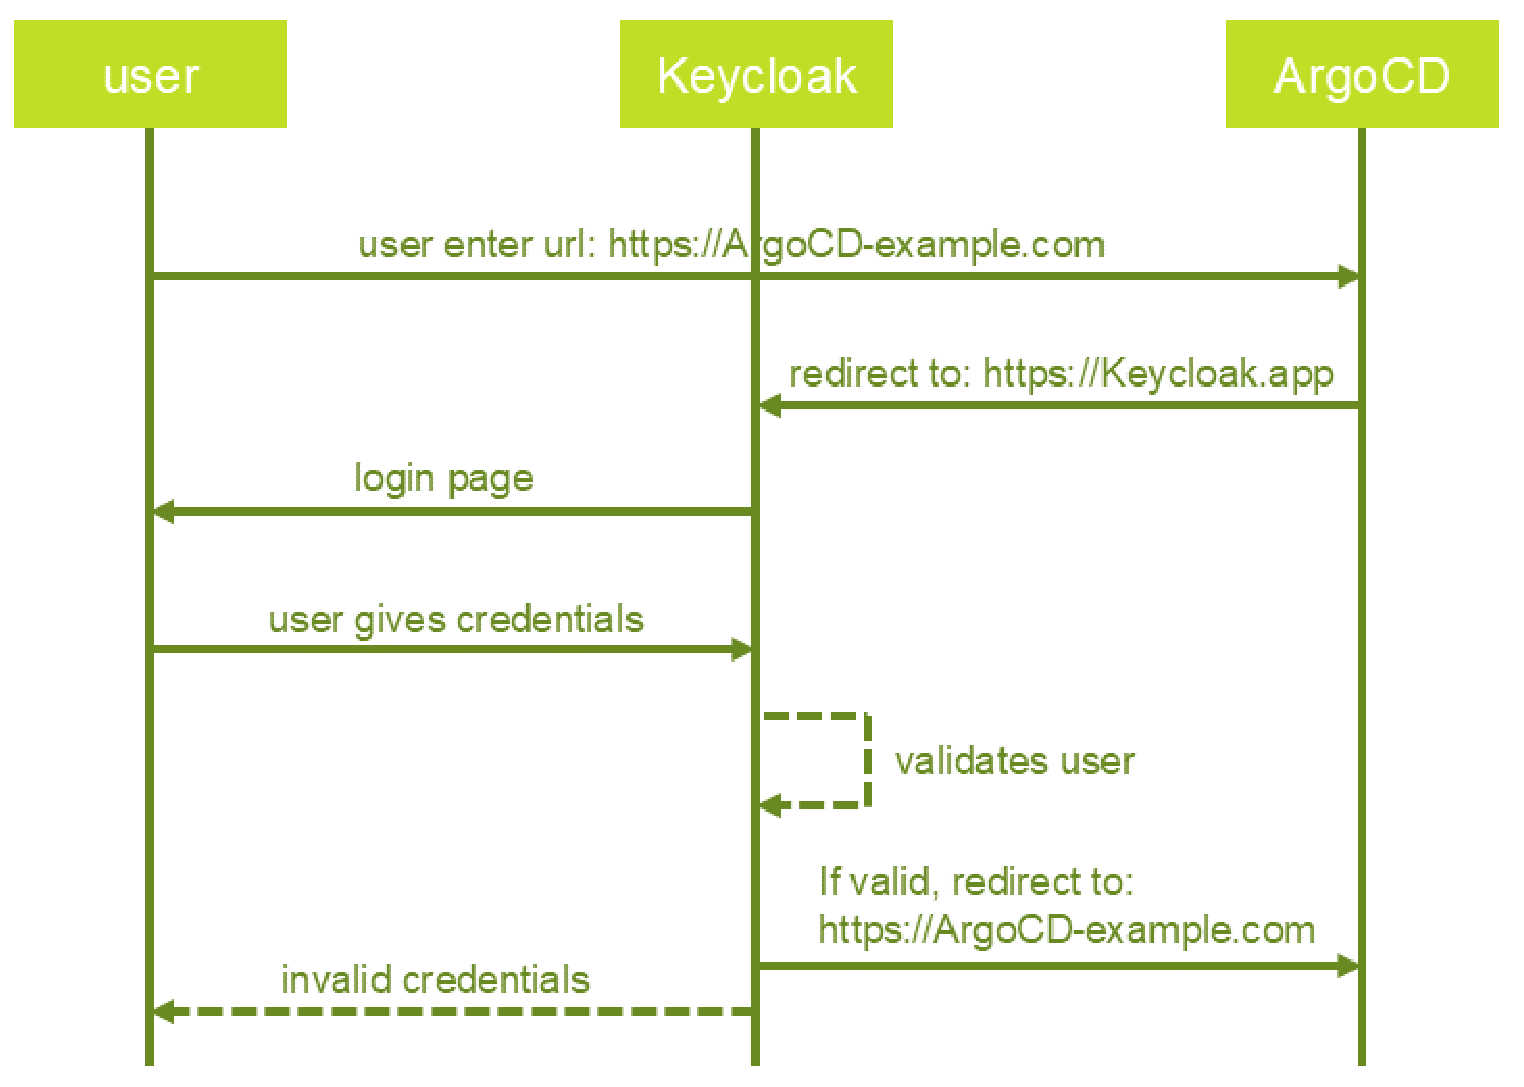
\includegraphics[width=1 \linewidth]{Thesis/Figures/Slide46.pdf}
\caption{\label{fig:Keycloak OIDC}Authentication with OIDC Protocol \cite{mohsen_talal_openid_connect}}
\end{figure}


\subsection{Keycloak Setup}

The installation of Keycloak in the Kubernetes environment is an important measure to get the secure centralized authentication for applications including ArgoCD. Deploying Keycloak on a Kubernetes cluster leverages Kubernetes orchestration capabilities ensuring that Keycloak is resilient and can handle scaling automatically based on demand. The deployment uses the Keycloak quick start repository which provides ready to use configuration files for seamless integration with Kubernetes. These files allow administrators to quickly create the necessary deployments, services and ingress configurations to make Keycloak accessible both internally and externally. Additionally, Kubernetes ingress resources are configured to expose Keycloak securely to users providing a centralized authentication point for various services including ArgoCD as shown in \autoref{fig:Keycloak}. \cite{keycloak_quickstarts}

\clearpage

\begin{figure}[h]
\centering
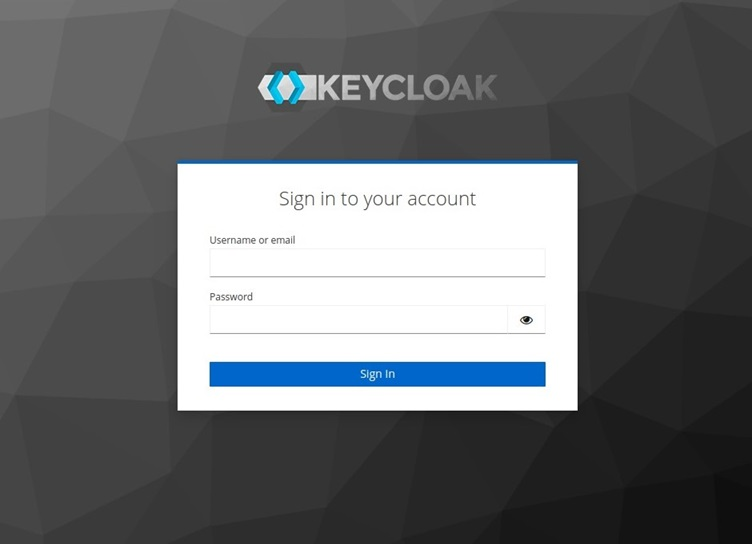
\includegraphics[width=0.8 \linewidth]{Thesis/Figures/Slide48.jpg}
\caption{\label{fig:Keycloak}Keycloak Authentication Interface}
\end{figure}



\textbf{Create New Realm and Client in Keycloak}

In Keycloak, a realm is a fundamental building block that isolates configurations and user data, making it ideal for managing authentication for multiple applications in a secure manner. For this implementation, a new realm was created specifically for ArgoCD, ensuring that its authentication flows are isolated from other applications, which enhances security and simplifies management. Within the new realm, a client representing ArgoCD was configured. The client is essential because it defines how ArgoCD interacts with Keycloak using the OIDC protocol, which provides a secure and standardized way of handling authentication. \autoref{fig:Keycloak client} illustrating the client creation in Keycloak for ArgoCD. \cite{openid-connect-core-1_0, keycloak_doc}


\begin{figure}[h]
\centering
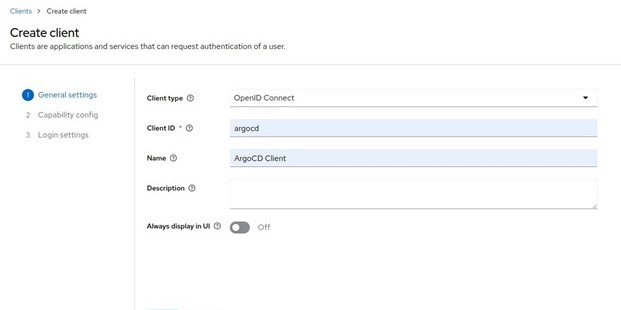
\includegraphics[width=0.86 \linewidth]{Thesis/Figures/Slide47.jpg}
\caption{\label{fig:Keycloak client}Creating Client in Keycloak}
\end{figure}

\clearpage

\textbf{Configure Root, Web and Admin URL}

When configuring a client in Keycloak, you need to set several URLs, including the Root URL, Web Origins and Admin URL as shown in \autoref{fig:Keycloak url}. The Root URL should be set to the base URL of your application, which Keycloak will use for redirects during authentication. The Web Origins field specifies allowed domains, ensuring that only the specified origins can interact with Keycloak from the browser. The Admin URL is used by Keycloak to send administrative actions, such as session invalidation, to the client. By setting all these URLs to the host name of your application, you establish a secure connection between Keycloak and your application for both frontend interaction and backend administration. \cite{keycloak_doc}

\begin{figure}[h]
\centering
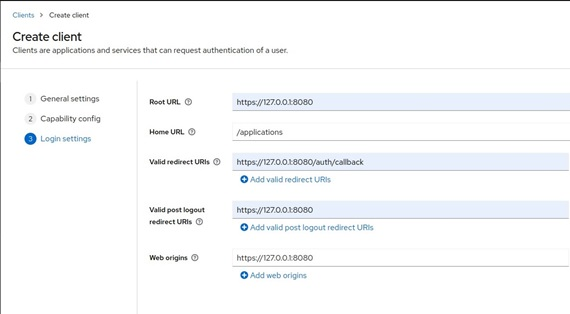
\includegraphics[width=0.75 \linewidth]{Thesis/Figures/Slide51.jpg}
\caption{\label{fig:Keycloak url}Configure Root, Web and Admin URL}
\end{figure}

\textbf{Configure Client Secret, Roles and Users within Keycloak}

A client secret was generated for the ArgoCD client, ensuring that only authorized services can authenticate with Keycloak as shown in \autoref{fig:client secret}. This client secret acts as a secure credential that is required whenever ArgoCD requests authentication tokens from Keycloak, reinforcing the security of the integration. \cite{keycloak_doc}

\begin{figure}[h]
\centering
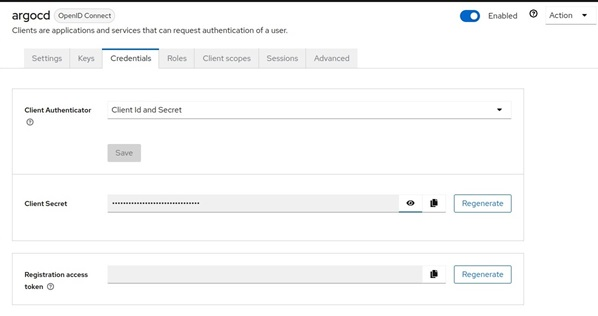
\includegraphics[width=0.7 \linewidth]{Thesis/Figures/Slide50.jpg}
\caption{\label{fig:client secret}Generating Client Secret in Keycloak}
\end{figure}

In order to implement fine-grained access control, roles have been defined within the Keycloak realm. These roles, such as admin, developer and viewer, encapsulate different levels of permissions, allowing for precise control over what users can do within ArgoCD. Assigning roles to users streamlines permission management and increases security by centralizing control within Keycloak. Finally, users were created and assigned the appropriate roles within Keycloak as shown in \autoref{fig:Keycloak user}. These users are the actual identities that will interact with ArgoCD and their roles determine their permissions, ensuring that access is tightly regulated based on organizational policies. \cite{keycloak_doc}


\begin{figure}[h]
\centering
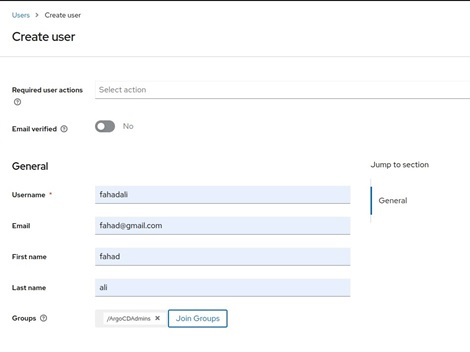
\includegraphics[width=0.8 \linewidth]{Thesis/Figures/Slide52.jpg}
\caption{\label{fig:Keycloak user}Creating User in Keycloak}
\end{figure}


\subsection{ArgoCD Configuration}

Configuring ArgoCD to use Keycloak as its OIDC provider involves several critical steps to ensure seamless authentication and secure integration between the two systems. The configuration focuses on modifying the ConfigMap and Secret within the Kubernetes cluster where ArgoCD is deployed, enabling it to authenticate users via Keycloak using the OIDC protocol for secure identity management and streamlined access. \cite{argocd_docs}


\textbf{Configuring ArgoCD to Use Keycloak as OIDC Provider}

To integrate Keycloak with ArgoCD, the first step is to configure client secret in ArgoCD to recognize Keycloak as its external identity provider using the client secret generated in Keycloak in the previous section. This process involves storing the client secret in the \texttt{argocd-secret}, which is the main secret used by ArgoCD for configuration. Begin by encoding the Keycloak client secret in base64 format then you need to edit the \texttt{argocd-secret} to include the base64 encoded client secret. This secret will be stored under a new key called \texttt{oidc.keycloak.clientSecret} as shown in code snippet \autoref{listingsnippet:5}. This modification allows ArgoCD to securely communicate with Keycloak as an external identity provider. \cite{argocd_docs}


\listingsnippet{Client Secret \cite{argocd_docs}}{

\vspace{0.3cm}

\hspace{0.25cm}\texttt{apiVersion: v1}

\hspace{0.25cm}\texttt{kind: Secret}

\hspace{0.25cm}\texttt{metadata:}

\hspace{0.5cm}\texttt{name: ArgoCD-secret}

\hspace{0.25cm}\texttt{data:}

\hspace{0.5cm}...

\hspace{0.5cm}\texttt{oidc.keycloak.clientSecret: <base64-encoded-client-secret>}

\hspace{0.5cm}...

\vspace{0.3cm}
}

To complete the integration of Keycloak with ArgoCD, the next step is to configure the ArgoCD ConfigMap to include the OIDC configuration that enables Keycloak authentication. In addition, we will set up access policies in ArgoCD to define roles for users authenticated by Keycloak. After updating the \texttt{argocd-cm} ConfigMap, the ConfigMap should look like code snippet \autoref{listingsnippet:6}. \cite{argocd_docs}

\listingsnippet{Configuring ConfigMap \cite{argocd_docs}}{

\vspace{0.3cm}

\hspace{0.25cm}\texttt{apiVersion: v1}

\hspace{0.25cm}\texttt{kind: ConfigMap}

\hspace{0.25cm}\texttt{metadata:}

\hspace{0.75cm}\texttt{name: argocd-cm}

\hspace{0.25cm}\texttt{data:}

\hspace{0.75cm}\texttt{oidc.config:}

\hspace{1.5cm}\texttt{name: keycloak}

\vspace{0.1cm}
  
\hspace{1.5cm}\texttt{issuer: http://192.168.49.2:30965/realms/argocd}

\vspace{0.1cm}
    
\hspace{1.5cm}\texttt{clientID: ArgoCD}

\vspace{0.1cm}
    
\hspace{1.5cm}\texttt{clientSecret: oidc.keycloak.clientSecret}

\vspace{0.1cm}
    
\hspace{1.5cm}\texttt{requestedScopes: ["openid", "profile", "email", "groups"]}

\vspace{0.1cm}
  
\hspace{0.75cm}\texttt{url: https://127.0.0.1:8080}

  \vspace{0.3cm}
}

In OIDC configuration it is required to define Issuer URL, ClientID, Client Secret and Scope. In which \texttt{issuer} URL is the endpoint of the Keycloak realm that ArgoCD will use to authenticate users. The \texttt{issuer} field must point to the Keycloak realm. The \texttt{clientID} corresponds to the client configured in Keycloak, which represents ArgoCD. The \texttt{clientSecret} is securely stored and used to authenticate the OIDC requests between ArgoCD and keycloak.
The \texttt{requestedScopes} field defines the permissions that ArgoCD requests from Keycloak, including standard OIDC scopes like \texttt{openid}, \texttt{profile}, \texttt{email} and \texttt{groups}. These scopes allow ArgoCD to obtain necessary user information and group memberships, which are then mapped to ArgoCD roles. \cite{argocd_docs}

\clearpage

After updating the ConfigMap with the OIDC configuration, it is essential to apply the changes to the Kubernetes cluster to activate the new settings \cite{argocd_docs}. Following the restart, users will see a \autoref{fig:login via keycloak} button on the ArgoCD landing page, indicating the successful integration of Keycloak as the identity provider for ArgoCD \cite{argocd_docs}. This button allows users to start the authentication process through Keycloak, enabling secure and centralized access control for ArgoCD \cite{argocd_docs}. When users attempt to log into ArgoCD, they will be redirected to the Keycloak login page to authenticate using their Keycloak credentials \cite{keycloak_doc}. After successful authentication, Keycloak redirects users back to ArgoCD, where authorization is managed based on the roles and claims provided by Keycloak \cite{keycloak_doc}.

\begin{figure}[h]
\centering
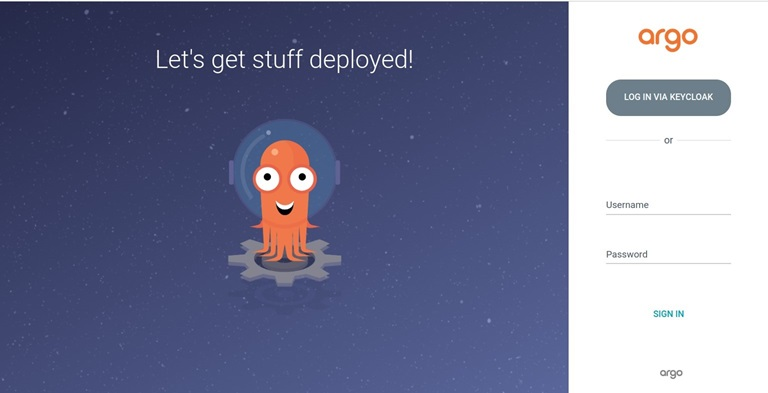
\includegraphics[width=1 \linewidth]{Thesis/Figures/Slide49.jpg}
\caption{\label{fig:login via keycloak}ArgoCD Login Via Keycloak}
\end{figure}

\subsection{Testing the Integration}

Having successfully configured ArgoCD to use Keycloak for SSO using OIDC protocol, the next step is to test the integration by logging into ArgoCD using Keycloak authentication. To begin testing, users will navigate to the ArgoCD web interface. On reaching the login page, they should now see an option to log in via Keycloak, indicating that the integration is active. Selecting the \texttt{Login via Keycloak} button will take users to the Keycloak authentication page where they enter their credentials. Once authenticated, Keycloak redirects the user back to ArgoCD, which processes the login and grants access based on the users roles and permissions as defined in Keycloak. A successful login indicates that the integration is working as expected and that all configurations between ArgoCD and Keycloak are correctly aligned.

\clearpage

\subsection{Challenges and Solutions}

During the integration process, several challenges arise that impact the functionality of the authentication system. One common issue is mismatched configurations between ArgoCD and Keycloak, particularly in the OIDC settings such as client ID, secret and redirect URIs. Ensuring that these configurations match exactly in both Keycloak and ArgoCD is crucial to avoiding authentication errors \cite{oauth_oidc_intro}. This issue is resolved by carefully reviewing the OIDC configuration in both platforms and ensuring they align with each other \cite{keycloak_doc}. Another challenge often encountered involves SSL/TLS certificates. ArgoCD and Keycloak both rely on secure HTTPS connections and any misconfiguration in SSL/TLS settings can result in failed connections between the two services. This problem can manifest as errors during the redirect process or outright failures to establish a secure session \cite{Kubernetes_doc}. The solution typically involves ensuring that valid SSL/TLS certificates are installed and properly configured in both Keycloak and ArgoCD, along with verifying that the correct certificate authorities are trusted by both systems \cite{argocd_docs}.

\section{Implementation of Authorization with Role-Based Access Control}

The implementation of RBAC in a Kubernetes cluster is critical to manage and secure access to resources. It provides a mechanism to define roles and assign permissions to users or groups using those roles. This approach is crucial in a multi-tenant environment where different users and applications require varying levels of access. By implementing RBAC, the cluster can enforce the principle of least privilege ensuring that users and services have only the permissions they need to perform their functions, thus reducing the risk of accidental or malicious actions. In Kubernetes RBAC is a built-in authorization mechanism that controls access to the API server and its resources. It uses four main concepts Roles, ClusterRoles, RoleBindings and ClusterRoleBindings. \cite{Kubernetes_doc}

\textbf{Roles and ClusterRoles} 

A Role and ClusterRole define a set of permissions where a Role is namespace scoped and ClusterRole is cluster-scoped. These permissions define which operations like Get, List, Create or Delete is allowed on certain resources such as Pods, Services, or Deployments. \cite{Kubernetes_doc}

\textbf{RoleBindings and ClusterRoleBindings} 

RoleBindings and ClusterRoleBindings are used to assign Roles or ClusterRoles to users or groups. A RoleBinding assigns a Role to a user within a specific namespace, while a ClusterRoleBinding assigns a ClusterRole to a user across the entire cluster. This separation of roles and bindings provides flexibility in how permissions are managed and assigned, allowing administrators to apply broad or narrow access controls as needed. Implementing RBAC in a Kubernetes cluster typically involves defining these roles and bindings in yet another markup language \abk{YAML}{Yet Another Markup Language} manifests, which are then applied to the cluster. For example, an administrator might create a role that allows read-only access to pods within a specific namespace and then bind that role to a group of developers. This ensures that the developers can view the pods but cannot modify or delete them, aligning their access level with their responsibilities. The configuration and management of RBAC are supported by tools like \texttt{kubectl}, which allows administrators to define and apply roles and bindings through command line operations. Additionally, RBAC policies can be dynamically updated as organizational needs evolve, ensuring that access controls remain aligned with the current security posture. \cite{Kubernetes_doc}

\subsection{Creating Roles and RoleBindings}

In RBAC system roles are created to assign permissions inside a namespace, as well as RoleBinding which is used to bind roles to users. Roles determine a given set of rights that outlines the kind of operations permitted on a set of objects in a namespace. For example, a Role might grant permissions to manage pods, services and deployments. This granularity ensures that users or service accounts have precise access based on their responsibilities. To define a Role, a YAML manifest is used, code snippet \autoref{listingsnippet:7} shows configuration for a example role named \texttt{developer-role}. \cite{Kubernetes_doc}

\listingsnippet{Role Configuration \cite{Kubernetes_doc}}{

\vspace{0.3cm}

\hspace{0.25cm}\texttt{apiVersion: rbac.authorization.k8s.io/v1}

\hspace{0.25cm}\texttt{kind: Role}

\hspace{0.25cm}\texttt{metadata:}

\hspace{0.75cm}\texttt{name: developer-role}

\hspace{0.75cm}\texttt{namespace: development}

\hspace{0.25cm}\texttt{rules:}

\hspace{0.25cm}\texttt{- apiGroups: [""]}

\hspace{0.75cm}\texttt{resources: ["pods", "services", "deployments"]}

\hspace{0.75cm}\texttt{verbs: ["get", "list", "create", "update", "delete"]}

\vspace{0.3cm}

}

Above YAML configuration grants permissions to manage pods, services and deployments within the \texttt{development} namespace. The \texttt{verbs} field specifies the actions allowed like get, list, create, update and delete. RoleBindings link the defined role to specific users, groups or service accounts within the namespace. This binding ensures that only the specified entities can perform the actions defined in the Role. For instance, code snippet \autoref{listingsnippet:8} shows YAML manifest to creates a RoleBinding that assign the \texttt{developer-role} to a user named \texttt{alice}. This RoleBinding guarantees that the user \texttt{alice} is granted the permissions defined in the \texttt{developer-role} for the \texttt{development} namespace. \cite{Kubernetes_doc} 

\listingsnippet{RoleBinding Configuration \cite{Kubernetes_doc}}{

\vspace{0.3cm}

\hspace{0.25cm}\texttt{apiVersion: rbac.authorization.k8s.io/v1}

\hspace{0.25cm}\texttt{kind: RoleBinding}

\hspace{0.25cm}\texttt{metadata:}

\hspace{0.75cm}\texttt{name: developer-role-binding}
  
\hspace{0.75cm}\texttt{namespace: development}
  
\hspace{0.25cm}\texttt{subjects:}

\hspace{0.25cm}\texttt{- kind: User}

\hspace{0.75cm}\texttt{name: alice}
  
\hspace{0.75cm}\texttt{apiGroup: rbac.authorization.k8s.io}

\hspace{0.25cm}\texttt{roleRef:}

\hspace{0.75cm}\texttt{kind: Role}
  
\hspace{0.75cm}\texttt{name: developer-role}
  
\hspace{0.75cm}\texttt{apiGroup: rbac.authorization.k8s.io}

\vspace{0.3cm}
}



\subsection{Creating ClusterRoles and ClusterRoleBindings}

ClusterRoles are used to define permissions that span across the entire Kubernetes cluster or across multiple namespaces. Unlike Roles, which are namespace scoped, ClusterRoles are cluster-scoped and are used for tasks that require broader access. Code snippet \autoref{listingsnippet:9} shows YAML configuration for a ClusterRole. \cite{Kubernetes_doc}


\listingsnippet{ClusterRole Configuration \cite{Kubernetes_doc}}{
\vspace{0.3cm}

\hspace{0.25cm}\texttt{apiVersion: rbac.authorization.k8s.io/v1}

\hspace{0.25cm}\texttt{kind: ClusterRole}

\hspace{0.25cm}\texttt{metadata:}

\hspace{0.75cm}\texttt{name: cluster-admin}

\hspace{0.25cm}\texttt{rules:}

\hspace{0.25cm}\texttt{- apiGroups: [""]}

\hspace{0.75cm}\texttt{resources: ["pods", "services", "deployments", "nodes"]}

\hspace{0.75cm}\texttt{verbs: ["get", "list", "create", "update", "delete"]}
\vspace{0.3cm}
}

The \texttt{cluster-admin} ClusterRole grants permissions to manage pods, services, deployments and nodes across the entire cluster . This role is essential for administrative functions that require cluster-wide access. ClusterRoleBindings bind ClusterRoles to users, groups, or service accounts, granting them the defined permissions across all namespaces. Code snippet \autoref{listingsnippet:10} shows the following YAML manifest creates a ClusterRoleBinding that assigns the \texttt{cluster-admin} ClusterRole to a user named \texttt{admin-user}. \cite{Kubernetes_doc}

\listingsnippet{ClusterRoleBinding Configuration \cite{Kubernetes_doc}}{
\vspace{0.3cm}

\hspace{0.25cm}\texttt{apiVersion: rbac.authorization.k8s.io/v1}

\hspace{0.25cm}\texttt{kind: ClusterRoleBinding}

\hspace{0.25cm}\texttt{metadata:}

\hspace{0.75cm}\texttt{name: cluster-admin-binding}

\hspace{0.25cm}\texttt{subjects:}

\hspace{0.25cm}\texttt{- kind: User}

\hspace{0.75cm}\texttt{name: admin-user}

\hspace{0.75cm}\texttt{apiGroup: rbac.authorization.k8s.io}
  
\hspace{0.25cm}\texttt{roleRef:}

\hspace{0.75cm}\texttt{kind: ClusterRole}
  
\hspace{0.75cm}\texttt{name: cluster-admin}
  
\hspace{0.75cm}\texttt{apiGroup: rbac.authorization.k8s.io}
\vspace{0.3cm}
}

This ClusterRoleBinding ensures that the user \texttt{admin-user} has administrative privileges across the entire Kubernetes cluster . By configuring these roles and bindings, administrators can effectively manage permissions, ensuring appropriate access levels while maintaining the security and integrity of the cluster. \cite{Kubernetes_doc}

\subsection{Automating Role-Based Access Control Authorization}

The automation of process of RBAC authorization consists of two steps first a private key and certificate signing request \abk{CSR}{Certificate Signing Request} is generated for the user and then in next step role and role binding or cluster role or cluster role binding is generated by automation script. \cite{Kubernetes_doc}

\textbf{User Creation}

The process of user creation begins with the generation of a private key and CSR specific to the user, which is essential for secure authentication. This CSR is then submitted to Kubernetes as a CSR object, which allows the user to be recognized as a system authenticated entity. The automation system handles the approval of the CSR, simulating the role of an administrator and retrieves the signed certificate upon approval. Once the certificate is issued, the system automatically configures the \texttt{kubeconfig} file by setting the users credentials and creating a new context that associates the user with the designated cluster and namespace. \cite{Kubernetes_doc}

\textbf{Creating Roles and Assigning it to Users}

The automated process of creating roles and binding them to users in a specified namespace, thereby streamlining access control within the cluster. The process begins by checking for the existence of the specified Role and RoleBinding to avoid duplication and ensure accurate configuration. It then automatically creates a Role with specific permissions, allowing the designated user to perform actions such as \texttt{get}, \texttt{list} and \texttt{watch} pods within the specified namespace. Once the role has been defined, the process creates a RoleBinding that associates the role with the user, thereby granting the appropriate permissions defined in the role. This automated approach ensures that access is consistently managed according to predefined security policies, reduces the potential for manual errors and facilitates efficient user management within Kubernetes environments, improving security and operational efficiency. This configuration allows the user to interact with the cluster in a secure manner and with the appropriate permissions as defined by the RBAC policies. The automated process significantly reduces manual intervention, ensures consistent user setup, minimises errors and increases the overall efficiency of managing access control in Kubernetes environments. \cite{Kubernetes_doc}

\subsection{Testing Role-Based Access Control}

Testing RBAC in Kubernetes involves verifying that users and service accounts can access only the resources and perform the actions they are authorized for, based on their assigned roles and role bindings. In this research different roles with varying permissions are defined and then assign these roles to different users or groups. For example, a user with an \texttt{admin} role should have full access to all resources, while a \texttt{developer} role might only have permissions to manage pods and services within a specific namespace. To validate the configuration, test were conducted by logging in as different users and attempting to perform operations that should be either allowed or denied according to their roles. For instance, a user assigned the \texttt{viewer} role should be able to view resources but should not be able to create or delete them, that show only the user with specific permissions and access levels, interact with the resources as intended. \cite{Kubernetes_doc}


\subsection{Challenges and Solutions}

Implementing RBAC can present several challenges, like overly permissive roles in which, one common issue is assigning overly broad permissions to roles, which might grant users more access than necessary. For example, if a \texttt{developer} role is mistakenly given \texttt{delete} permissions for all resources, it could lead to accidental or malicious deletion of critical resources. To mitigate this, carefully review and test role definitions and apply the principle of least privilege, granting only the permissions necessary for each role. Another challenge is creating incorrect or misconfigured RoleBindings and ClusterRoleBindings. For instance, binding a ClusterRole that has extensive permissions to a user who only needs limited access can pose a security risk. \cite{Kubernetes_doc}

\section{Implementation of Scalable Architectures}

Providing a scalable architecture for AI models is critical to meet the growing computational demands associated with modern ML workloads. In this implementation, Ray was chosen for its ability to handle distributed workloads making it an ideal choice for running AI models that require significant computational resources \cite{ray_doc}. To ensure both performance and cost efficiency the key objective was to create a system that could automatically adjust resources based on the workload. The deployment process began with the creation of a Kubernetes cluster which serves as the foundation for container orchestration and management \cite{Kubernetes_doc}. Kubernetes was chosen for its scalability features and support for managing containerised applications in production environments \cite{r4}. The cluster was created using Kind, which makes it easy to create a Kubernetes environment using Docker containers \cite{kind2021}. Once the Kubernetes cluster was in place then the next step was to deploy Ray on top of it. The Ray architecture allows tasks to scale seamlessly across multiple nodes, ensuring efficient use of resources \cite{ray_doc}. The Ray cluster was deployed using KubeRay, an operator that simplifies the management of Ray clusters on Kubernetes \cite{ray_doc}. KubeRay automates the provisioning, scaling and management of Ray clusters, which was essential for maintaining a stable and scalable environment \cite{burns2021designing}. To enable autoscaling, the Ray cluster was configured with autoscaling capabilities using KubeRay \cite{ray_doc}. Autoscaling is a critical feature that dynamically adjusts the number of worker nodes in the Ray cluster based on workload demands \cite{Kubernetes_doc}. This ensures that the cluster scales up when demand for compute resources is high, and scales down when demand decreases, optimising both performance and cost \cite{liu2019scalable}. The autoscaling configuration was defined in a YAML file, specifying the minimum and maximum number of worker nodes and the conditions under which scaling should occur \cite{ray_doc}. In addition to autoscaling, the Ray cluster was configured to support GPU access, which is essential for AI workloads involving large models \cite{wong2021gpu}. GPU support was enabled by specifying GPU resources in the Ray cluster configuration, allowing the cluster to use hardware accelerators for faster computation \cite{nvidia_gpu_operator}. This configuration was particularly important for training large neural networks, which require significant computing power \cite{goodfellow2016deep}. The final step was to validate the deployment by running AI model training tasks on the Ray cluster. The tasks were distributed across multiple nodes, with the autoscaler dynamically adjusting resources as needed \cite{spark_unified_engine}. This deployment successfully demonstrated the ability to scale AI model execution in a production like environment, meeting the objective of creating a scalable and efficient architecture for AI workloads \cite{dean2008mapreduce}.

\subsection{Ray on Kubernetes}

Ray cluster utilize Kubernetes orchestration capabilities to manage distributed computing tasks efficiently. Deploying Ray in a Kubernetes environment enables the scaling and management of complex AI workflows by leveraging Kubernetes features such as resource management, fault tolerance and automated scaling. This setup integrates distributed components of Ray, like Ray Core, Ray Data, Ray Train and Ray Tune within Kubernetes to handle large-scale ML tasks effectively. The synergy between Ray distributed computing framework and Kubernetes container orchestration facilitates a scalable and resilient infrastructure for AI applications \cite{moritz}. KubeRay extends this integration by providing an operator specifically designed to manage Ray clusters within Kubernetes. The KubeRay operator automates the deployment, scaling and management of Ray resources, each Ray cluster consisting of a head node and a collection of worker nodes, as shown in \autoref{fig:Ray on Kubernetes}. Ray clusters adapt dynamic Kubernetes environment by handling tasks such as autoscaling and GPU resource management, which provides support for adding or removing pods as needed. Thus, Kubernetes provides the basic orchestration, KubeRay complements it by streamlining the management of Ray distributed tasks, ultimately enabling efficient and scalable AI workload management. \cite{ray_doc}

\clearpage

\begin{figure}[h]
\centering
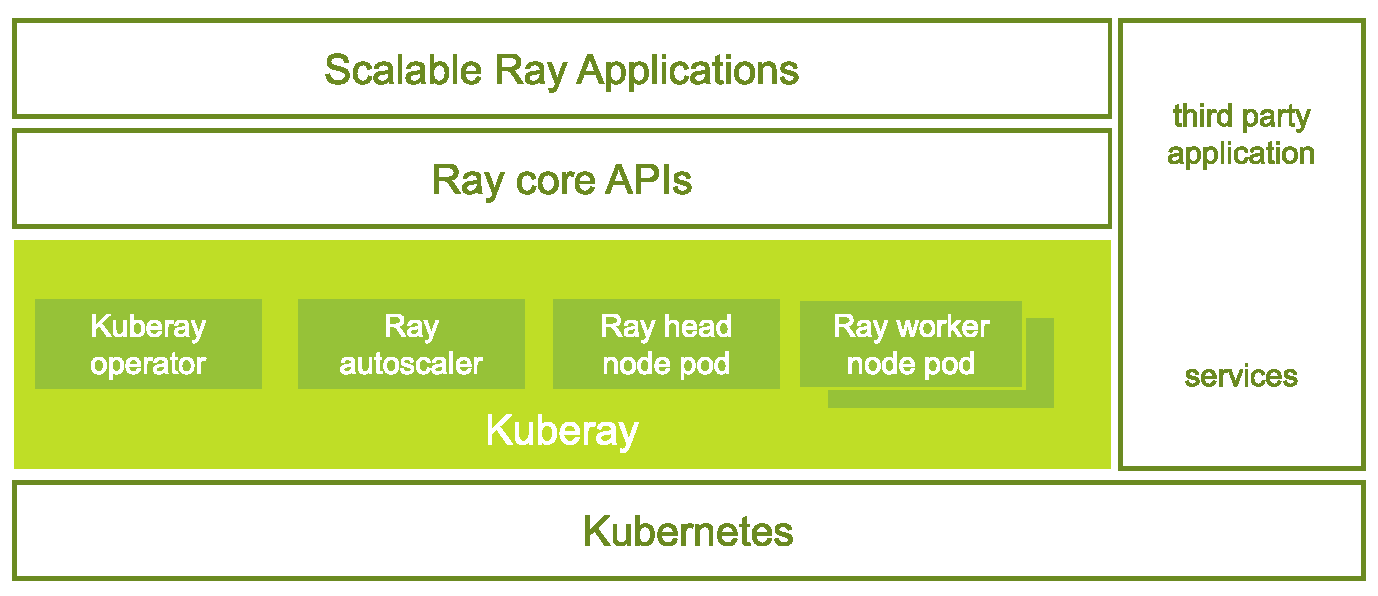
\includegraphics[width=1 \linewidth]{Thesis/Figures/Slide54.pdf}
\caption{\label{fig:Ray on Kubernetes}Ray on Kubernetes \cite{ray_doc}}
\end{figure}



\subsection{Setup Ray Cluster}

Setting up a Ray cluster within a Kubernetes environment requires several dependencies to ensure seamless integration and functionality. The initial step involves installing essential software, including Kubernetes and its associated tools like \texttt{kubectl}, which is necessary for managing the Kubernetes environment \cite{Kubernetes_doc}. Additionally, Docker is required to containerize the Ray components, while Helm is used to manage Kubernetes applications through Helm charts \cite{helm_docs}. For local Kubernetes cluster setup, tools such as kind can be utilized to create a lightweight, local cluster for development and testing purposes \cite{kind2021}. These dependencies are fundamental for creating a robust and scalable Ray cluster that can efficiently handle distributed computing tasks. The installation process for Ray involves deploying core Ray components and configuring them for Kubernetes integration. Start by installing the Ray core component, which forms the backbone of the Ray distributed computing framework. This is followed by the installation of Ray data for handling large datasets, Ray train for training ML models and Ray tune for hyperparameter tuning \cite{ray_doc}. Additional methods such as Ray actor and Ray job facilitate the management and execution of tasks and jobs within the Ray cluster \cite{ray_doc}. To integrate Ray with Kubernetes, KubeRay is deployed, which includes setting up the KubeRay operator. This operator manages the lifecycle of Ray clusters within Kubernetes \cite{ray_doc}. The configuration involves updating Ray autoscaler settings and applying them through Kubernetes manifests, ensuring that the cluster scales dynamically based on workload demands \cite{ray_doc}. By following these steps, the Ray cluster is set up to leverage Kubernetes orchestration capabilities, providing a scalable and efficient environment for running AI and ML workloads.

\subsection{KubeRay Autoscaling}

KubeRay uses Kubernetes HPA for dynamic resource management in Ray clusters. This integration ensures that Ray clusters can automatically adjust their size based on the workload according to the ratio of the current metric value to optimise resource utilization and maintain cluster performance. \cite{Kubernetes_doc}

\textbf{Horizontal Pod Autoscaling}

HPA is used to scale number of worker pods in a deployment based on observed metrics such as CPU utilization or any custom metrics \cite{Kubernetes_doc}. For Ray clusters, configuring HPA allows the number of Ray worker pods to automatically scale up or down in response to automatically adjust the load and ensuring that resources are allocated and used efficiently \cite{Kubernetes_doc}. The configuration of HPA required to achieve autoscaling is shown in code snippet \autoref{listingsnippet:11}.

\listingsnippet{HPA Configuration within Ray  \cite{ray_doc}}{

\vspace{0.3cm}

\hspace{0.25cm}\texttt{apiVersion: autoscaling/v2beta2}

\hspace{0.25cm}\texttt{kind: HorizontalPodAutoscaler}

\hspace{0.25cm}\texttt{metadata:}

\hspace{0.75cm}\texttt{name: ray-worker-hpa}

\hspace{0.75cm}\texttt{namespace: default}

\hspace{0.25cm}\texttt{spec:}

\hspace{0.75cm}\texttt{scaleTargetRef:}

\hspace{1.5cm}\texttt{apiVersion: apps/v1}

\hspace{1.5cm}\texttt{kind: Deployment}

\hspace{1.5cm}\texttt{name: ray-worker}

\hspace{0.75cm}\texttt{minReplicas: 2}

\hspace{0.75cm}\texttt{maxReplicas: 10}

\hspace{0.75cm}\texttt{metrics:}

\hspace{0.75cm}\texttt{- type: Resource}
    
\hspace{1.5cm}\texttt{resource:}
    
\hspace{2cm}\texttt{name: cpu}

\hspace{2cm}\texttt{target:}

\hspace{2.5cm}\texttt{type: Utilization}

\hspace{2.5cm}\texttt{averageUtilization: 50}

\vspace{0.3cm}
}


This configuration ensures that the number of Ray worker pods is adjusted between 2 and 10 based on the average CPU utilization. By setting these parameters, the HPA maintains an optimal number of pods to handle varying workloads efficiently. \cite{Kubernetes_doc}

\textbf{Detached and Terminate Detached Actors}

Ray actor model supports detached and terminated detached actors, which are essential for managing long running and stateful tasks within a Ray cluster. Detached and terminate detached actors continue to operate independently of the cluster lifecycle, which allows for continuity in ongoing computations even during scaling events. Detached actors are designed to persist across scaling or restart events. They continue executing their tasks and maintaining their state, which is crucial for computations that require continuity. To manage resources effectively, detached actors can be terminated when they are no longer needed. This ensures that resources are reclaimed and utilized efficiently during scaling events. \cite{ray_doc}

\clearpage

\textbf{Hyperparameter Tuning Trials with Ray Tune}

In this phase of the implementation, the autoscaling process was tested by varying the number of hyperparameter tuning trials. As the volume of trials increased, the computational load on the Ray cluster also increased, thereby necessitating the scaling of the worker pods. The underlying principle involves scaling the number of Ray worker pods based on the demands of the hyperparameter tuning process. The \texttt{tune.run()} function configuration in Kubernetes, as shown in the code snippet \autoref{listingsnippet:12}, was used to tune hyperparameters, initiated multiple hyperparameter search trials, which impacted the workload and triggered autoscaling to manage the increased demand. The HPA monitored CPU utilization and adjusted the number of pods accordingly, ensuring that the cluster could handle the computational load efficiently. \cite{ray_doc}

\listingsnippet{Hyperparameter Tuning Trials with Ray Tune \cite{ray_doc}}{
\vspace{0.3cm}

\hspace{0.25cm}\texttt{\# Configure Ray Tune}

\vspace{0.3cm}

\hspace{0.25cm}\texttt{analysis = tune.run(}

\vspace{0.3cm}

\hspace{0.75cm}\texttt{train-model,}

\hspace{0.75cm}\texttt{config=search-space,}

\hspace{0.75cm}\texttt{numsamples=10,}

\hspace{0.75cm}\texttt{metric="metric",}

\hspace{0.75cm}\texttt{mode="max",}

\hspace{0.75cm}\texttt{resources-per-trial={"cpu": 1},}

\hspace{0.75cm}\texttt{verbose=1,}

\vspace{0.3cm}

\texttt{)}
    
\vspace{0.3cm}  
}



\subsection{Ray cluster Autoscaling Workflow}

Enabling a scalable architecture with Ray involves several installation and configuration steps. Including creating a cluster, deploying the KubeRay operator, enabling autoscaling and installing dependencies. The workflow is designed to automate the process of configuring scalable Ray cluster on Kubernetes using Kind and KubeRay. The process starts with the creation of a custom Docker image initialize with the official Ray image and additional dependencies required by the model such as scikit-learn are added as shown in code snippet \autoref{listingsnippet:13}. This Docker image is automatically built from a Docker file and pushed to a Docker registry for future use. In next step a Kubernetes cluster is created using Kind. Once the cluster is created, the workflow then deploys the KubeRay operator which manages Ray clusters within Kubernetes. The KubeRay Helm repository is then added and operator is deployed in a dedicated namespace to ensure efficient cluster management and scaling. After setting up the operator script updates Ray autoscaler configuration to use the custom Docker image created in the first step. The updated configuration makes sure that all the necessary dependencies is installed using Docker image. Then autoscaling configuration is applied to deploy a Ray cluster with autoscaling enabled. This allows the cluster to dynamically scale its resources with all the dependencies installed. Finally, the script monitors the deployment by continuously checking the pods in the specified namespace and verifying that everything is running as expected. This automated workflow allows ML engineers to efficiently set up a scalable computing environment using Ray clusters in Kubernetes simplifying resource management and automating scaling for computational tasks that require dynamic resource allocation.

\listingsnippet{Docker Images to Install Dependencies}{

\vspace{0.3cm}


\hspace{0.25cm}\texttt{\# Start from the official Ray image}

\hspace{0.25cm}\texttt{FROM rayproject/ray:2.9.0}

\vspace{0.3cm}

\hspace{0.25cm}\texttt{\# Install scikit-learn and any other dependencies you need}

\hspace{0.25cm}\texttt{RUN pip install scikit-learn}

\vspace{0.3cm}
}

\subsection{Installing Dependencies to Resources}



Installing dependencies in a containerized environment is essential to ensure that the application has all the required libraries and tools to function correctly. These dependencies, whether they are specific programming language libraries, system tools, or other runtime utilities, are vital for running the code within the container, without them the application might not start or could encounter errors during execution, leading to service disruptions. Properly managing and installing these dependencies not only ensures that the application works as expected but also enhances its portability and consistency across different environments. This becomes particularly important in dynamic environments, such as distributed computing, where resources are scaled up or down frequently and ensuring that the required dependencies are always available to maintain performance and functionality. Two primary methods to handle dependency installation in distributed environments is implemented in this research. \cite{Kubernetes_doc, loft2024adding}

\begin{itemize}
    \item Container image method
    \item Container lifecycle hooks
\end{itemize}

\textbf{Container Image Method}

In container image method, dependencies can be managed efficiently by creating a Docker file that lists and installs all the necessary libraries, system tools and other utilities required by the application. This Docker file can include commands such as \texttt{RUN pip install} for Python libraries or \texttt{RUN apt-get install} for system dependencies, ensuring that the container image is built with everything the application needs to run. Once the image is built, it is used in the pod's YAML configuration to ensure that the container starts with all dependencies preinstalled as shown in code snippet \autoref{listingsnippet:14}. When Kubernetes scales the application using HPA, it automatically deploys new worker pods using this pre-configured image, ensuring all dependencies are already installed on all worker nodes. This approach not only ensures consistency across environments, but also speeds up the startup process for new pods by eliminating the need for additional installations at runtime. With this configuration, Kubernetes can efficiently scale resources while maintaining reliable, independent environment for all pods. \cite{Kubernetes_doc, loft2024adding}

\listingsnippet{Updated Pod Configuration using Docker Image \cite{Kubernetes_doc}}{

\vspace{0.3cm}
 
\hspace{0.25cm}\texttt{headGroupSpec:}

\hspace{0.75cm}\texttt{rayStartParams:}

\hspace{1.25cm}\texttt{num-cpus: "0"}

\hspace{0.75cm}\texttt{template:}

\hspace{1.25cm}\texttt{spec:}

\hspace{1.75cm}\texttt{containers:}

\hspace{1.75cm}\texttt{- image: my-custom-ray:2.9.0}

\hspace{2.25cm}\texttt{lifecycle:}

\hspace{2.75cm}\texttt{preStop:}

\hspace{3,25cm}\texttt{exec:}

\hspace{3.75cm}\texttt{command:}

\hspace{3.75cm}\texttt{- /bin/sh}

\hspace{3.75cm}\texttt{- -c}

\hspace{3.75cm}\texttt{- ray stop}

\vspace{0.3cm}
}

\textbf{Container Lifecycle Hooks}


Container lifecycle hook allows containers to execute specific code and installation processes triggered by events during its administrative lifecycle. These hooks provide flexibility in handling actions during the container lifecycle by allowing containers to be aware of specific events and execute code when triggered. PostStart and PreStop are the two primary hooks exposed to containers. The PostStart hook is executed immediately after a container is created, allowing custom code to be executed when the container starts. This can be useful for installing dependencies or performing other setup tasks that need to occur at the start of the container, but after the image has been initialised. The hook can be configured in the pod's YAML configuration, as shown in the code snippet \autoref{listingsnippet:15}. 

\listingsnippet{Update Pod Configuration using PostStart Hooks \cite{Kubernetes_doc}}{

\vspace{0.3cm}
 
\hspace{0.25cm}\texttt{headGroupSpec:}

\hspace{0.75cm}\texttt{rayStartParams:}

\hspace{1.25cm}\texttt{num-cpus: "0"}

\hspace{0.75cm}\texttt{template:}

\hspace{1.25cm}\texttt{spec:}

\hspace{1.75cm}\texttt{containers:}

\hspace{1.75cm}\texttt{- image: rayproject/ray:2.9.0}

\hspace{2.25cm}\texttt{lifecycle:}

\hspace{2.75cm}\texttt{postStop:}

\hspace{3,25cm}\texttt{exec:}

\hspace{3.75cm}\texttt{command: ["/bin/bash", "-c", "/bin/setup-head.sh"]}

\vspace{0.3cm}
}

The second hook, PreStop, is executed just before the container is destroyed, typically triggered by events such as API requests or resource contention. The PreStop hook allows containers to handle termination gracefully by performing specific shutdown procedures, such as saving state or closing connections, before the container is stopped. Like the PostStart hook, the container will eventually terminate within its grace period, regardless of the outcome of the handler. An example configuration of the PreStop hook is shown in the code snippet at \autoref{listingsnippet:16}.





\listingsnippet{Update Pod Configuration using PreStop Hooks \cite{Kubernetes_doc}}{

\vspace{0.3cm}
 
\hspace{0.25cm}\texttt{workerGroupSpec:}

\hspace{0.75cm}\texttt{rayStartParams:}

\hspace{1.25cm}\texttt{num-cpus: "0"}

\hspace{0.75cm}\texttt{template:}

\hspace{1.25cm}\texttt{spec:}

\hspace{1.75cm}\texttt{containers:}

\hspace{1.75cm}\texttt{- image: rayproject/ray:2.9.0}

\hspace{2.25cm}\texttt{lifecycle:}

\hspace{2.75cm}\texttt{preStop:}

\hspace{3,25cm}\texttt{exec:}

\hspace{3.75cm}\texttt{command: ["/bin/bash", "-c", "/bin/setup-head.sh"]}

\vspace{0.3cm}
}

\subsection{GPU Access in KubeRay}

Accessing GPU is critical to achieve high performance in computing related to ML and deep learning \abk{DL}{Deep Learning} workloads \cite{nvidia_gpus_ai_ml}. GPU enables fast processing of large datasets and complex AI models and provides high processing power \cite{nvidia_gpus_ai_ml}. In KubeRay enabling GPU access involves several steps. First Kubernetes nodes must be equipped with GPUs and the necessary NVIDIA drivers and container runtime must be installed \cite{Kubernetes_doc}. Kubernetes uses the NVIDIA device plugin to expose GPUs to pods which must be properly configured in the Ray cluster setup \cite{Kubernetes_doc}. The Ray cluster configuration file must include resource requirements and limits for GPUs in the worker pod definitions. For example, in the YAML configuration file for the Ray cluster, you would specify the number of GPUs required by setting \texttt{nvidia.com/gpu} in the \texttt{resources} section of the worker pod configuration. This ensures that the Ray tasks requiring GPU resources are scheduled on nodes where GPUs are available \cite{ray_doc}. Configuration shows in code snippet \autoref{listingsnippet:17}, where each Ray worker pod is configured to request a GPU. This setup allows the Ray cluster to efficiently utilize GPU resources, thereby accelerating the processing of tasks that benefit from parallel computing, such as neural network training. \cite{ray_doc}

\listingsnippet{Ray Cluster Configuration with GPU Request \cite{ray_doc}}{

\vspace{0.3cm}

\hspace{0.25cm}\texttt{apiVersion: ray.io/v1alpha1}

\hspace{0.25cm}\texttt{kind: RayCluster}

\hspace{0.25cm}\texttt{metadata:}

\hspace{0.75cm}\texttt{name: ray-cluster}

\hspace{0.25cm}\texttt{spec:}

\hspace{0.75cm}\texttt{workerGroupSpecs:}

\hspace{1.5cm}\texttt{- replicas: 2}

\hspace{2cm}\texttt{template:}

\hspace{2.5cm}\texttt{spec:}

\hspace{3cm}\texttt{containers:}

\hspace{3.5cm}\texttt{- name: ray-worker}

\hspace{4cm}\texttt{image: rayproject/ray-ml:latest}

\hspace{4cm}\texttt{resources:}

\hspace{4.5cm}\texttt{limits:}

\hspace{5cm}\texttt{nvidia.com/gpu: 1}

\hspace{4.5cm}\texttt{requests:}

\hspace{5cm}\texttt{nvidia.com/gpu: 1}

\vspace{0.3cm}

}
                  
Furthermore, KubeRay supports dynamic scaling of GPU resources, aligning with the broader autoscaling capabilities of Ray clusters. This means that as the demand for GPU intensive tasks increases, KubeRay can scale the number of GPU equipped worker pods accordingly, ensuring that computational resources match the workload requirements. \cite{ray_doc}










            \chapter{Compare Ray Results with Other Distributed Computing Tools}

\vspace{0.3cm}
As outlined in the preceding chapter, the implementation of a scalable architectures for AI models utilizing Ray, a robust distributed computing framework, facilitates seamless autoscaling and the efficient distribution of computational resources within a cloud-native architectures \cite{moritz}. This chapter examined the ways in which the fundamental modules of Ray comprising Ray Data, Ray Tune, Ray Train, Ray Serve and RLlib facilitate distributed data processing, hyperparameter optimization, model training and serving tasks within a unified ecosystem. The objective of this chapter is to present a comprehensive comparison between the Ray ecosystem and other prominent tools in the distributed computing domain, including Apache Spark, Dask, Modin, Optuna, Hyperopt and TensorFlow Serve. This comparison is intended to highlight the different features and capabilities of Ray and to assist users in selecting the most appropriate framework based on their specific use cases whether they are focused on machine learning, data processing or large-scale computations \cite{ray_doc}.

\section{Distributed Computing Tools}


This section provides an overview of popular distributed computing frameworks, including Apache Spark, Hadoop, Modin, Dask, Optuna, Hyperopt and TensorFlow. These technologies are essential in supporting big data and are used to facilitate scalable data processing over distributed environments. They form the core of the distributed computing technology stack, allowing organisations to manage, process and analyse large volumes of data across clusters seamlessly and are therefore essential tools in modern big data applications.
 \cite{sun2023survey}


\subsection{Hadoop}
Apache Hadoop is an open source technology that creates an infrastructure for managing big data across multiple nodes or resources which makes it suitable for big data applications. The
Hadoop ecosystem is made of combining of different software packages it offers different functionality for different scenarios. For example Hadoop distributed file system \abk{HDFS}{Hadoop Distributed File System} manages process to store files in distributed manner, whereas Hadoop MapReduce is a software framework which helps to execute MapReduce algorithm for larger distributed datasets in clusters. These software components work together seamlessly in clusters or cloud-native environments to perform tasks for a variety of applications. Hadoop uses a master slave architecture to efficiently store and process large amounts of data. During task execution, the master node distributes sub tasks to the slave nodes, which store local blocks of data and perform computations on that data locally. \cite{ketu2020performance, sun2023survey}

\textbf{Hadoop Distributed File System}

HDFS is the block storage layer that Hadoop uses to manage its files, designed to handle very large datasets with high reliability. HDFS uses data replication to ensure data integrity and availability, this replication allows HDFS to efficiently stream large amounts of data to applications in a timely manner. Its architecture consists of two main components, the NameNode and the DataNodes, which operate in a master slave setup. The NameNode manages the metadata that tracks where files are stored in the system, while the DataNodes handle the actual data storage. HDFS operates as a single writer, multiple reader file system, meaning that once a client opens a file for writing, it has exclusive access until the operation is complete. Once a file is closed, its contents cannot be modified or removed, although additional data can be appended by reopening the file. Over time, HDFS has undergone numerous improvements that have increased its flexibility and enabled it to support different approaches to MapReduce computation. \cite{polato2014comprehensive}

\textbf{MapReduce}

A job in Hadoop consists primarily of two key functions, the map function and the reduce function. In addition, there are other functions that can be executed after the map function or between the map and reduce functions. The main role of the map function is to read chunks of data from HDFS and convert them into key/value pairs with different partitions. For example, in text mining, the map function acts as a parser and cleaner for the dataset, as shown \autoref{fig:MapReduce}, where the input data is divided among multiple mappers, followed by the reduce tasks to perform parallel computations. Also shown in \autoref{fig:MapReduce}, the output from the mapping stage is fed into various reducers. These reducers then process the input key/value pairs to perform operations such as summing or averaging the values. \cite{ketu2020performance}

\begin{figure}[h]
\centering
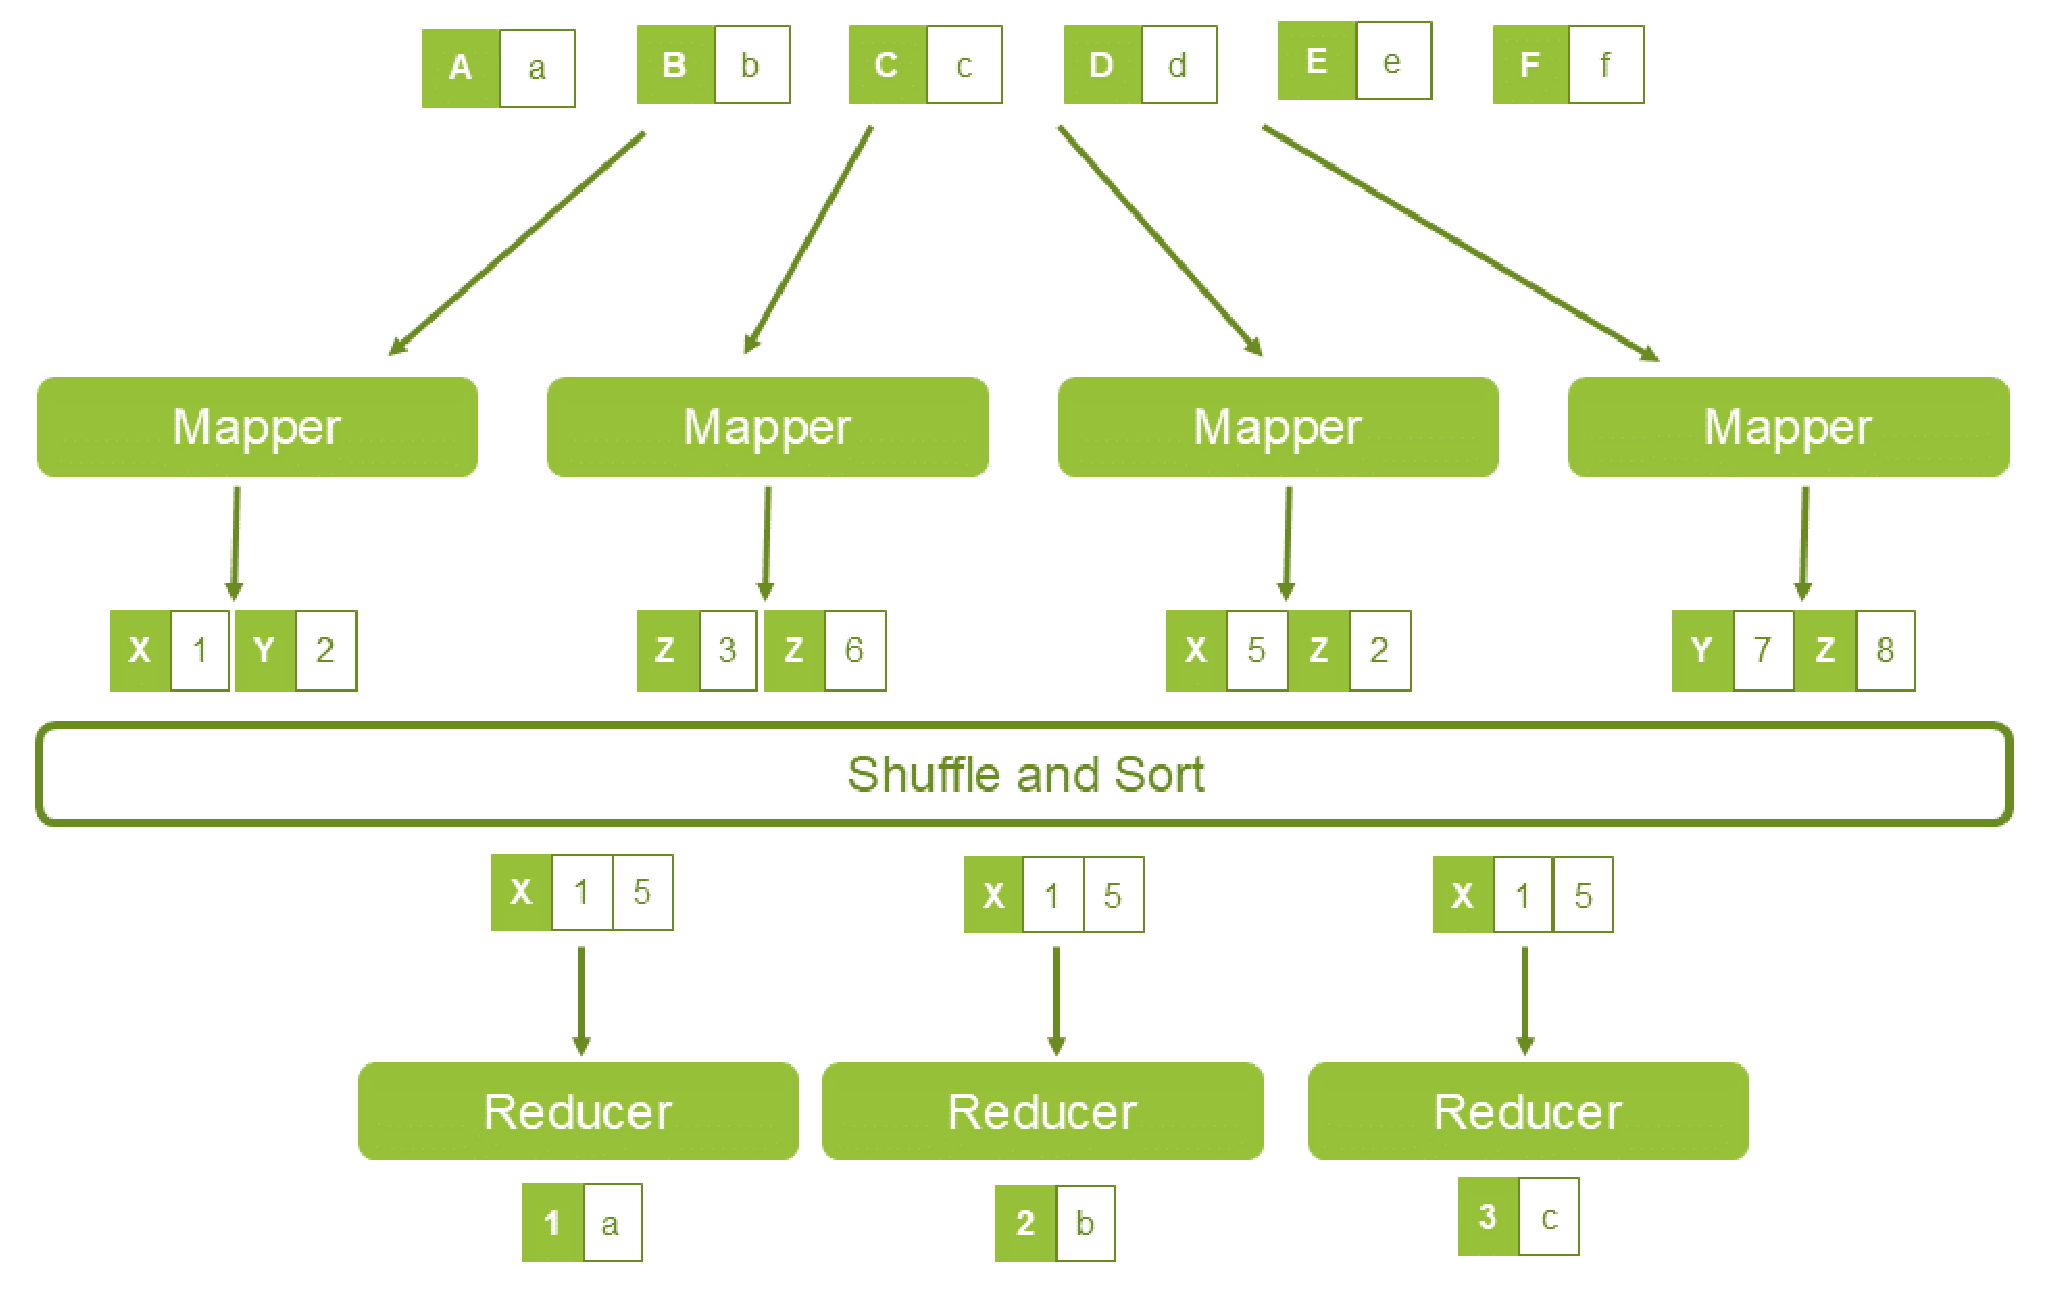
\includegraphics[width=1 \linewidth]{Thesis/Figures/Slide58.pdf}
\caption{\label{fig:MapReduce}MapReduce Programming
Model \cite{ketu2020performance}}
\end{figure}

The workflow of nodes in Hadoop is shown in \autoref{fig:hadoop}. Each MapReduce task is distributed across three nodes, the job submission node, the name node and the slave nodes, which ensure that the task is successfully completed. JobTracker and TaskTracker monitor the progress of the MapReduce tasks, while all operations are performed on DataNodes managed by the NameNode. These processes are executed within the slave nodes. \cite{ketu2020performance}

\begin{figure}[h]
\centering
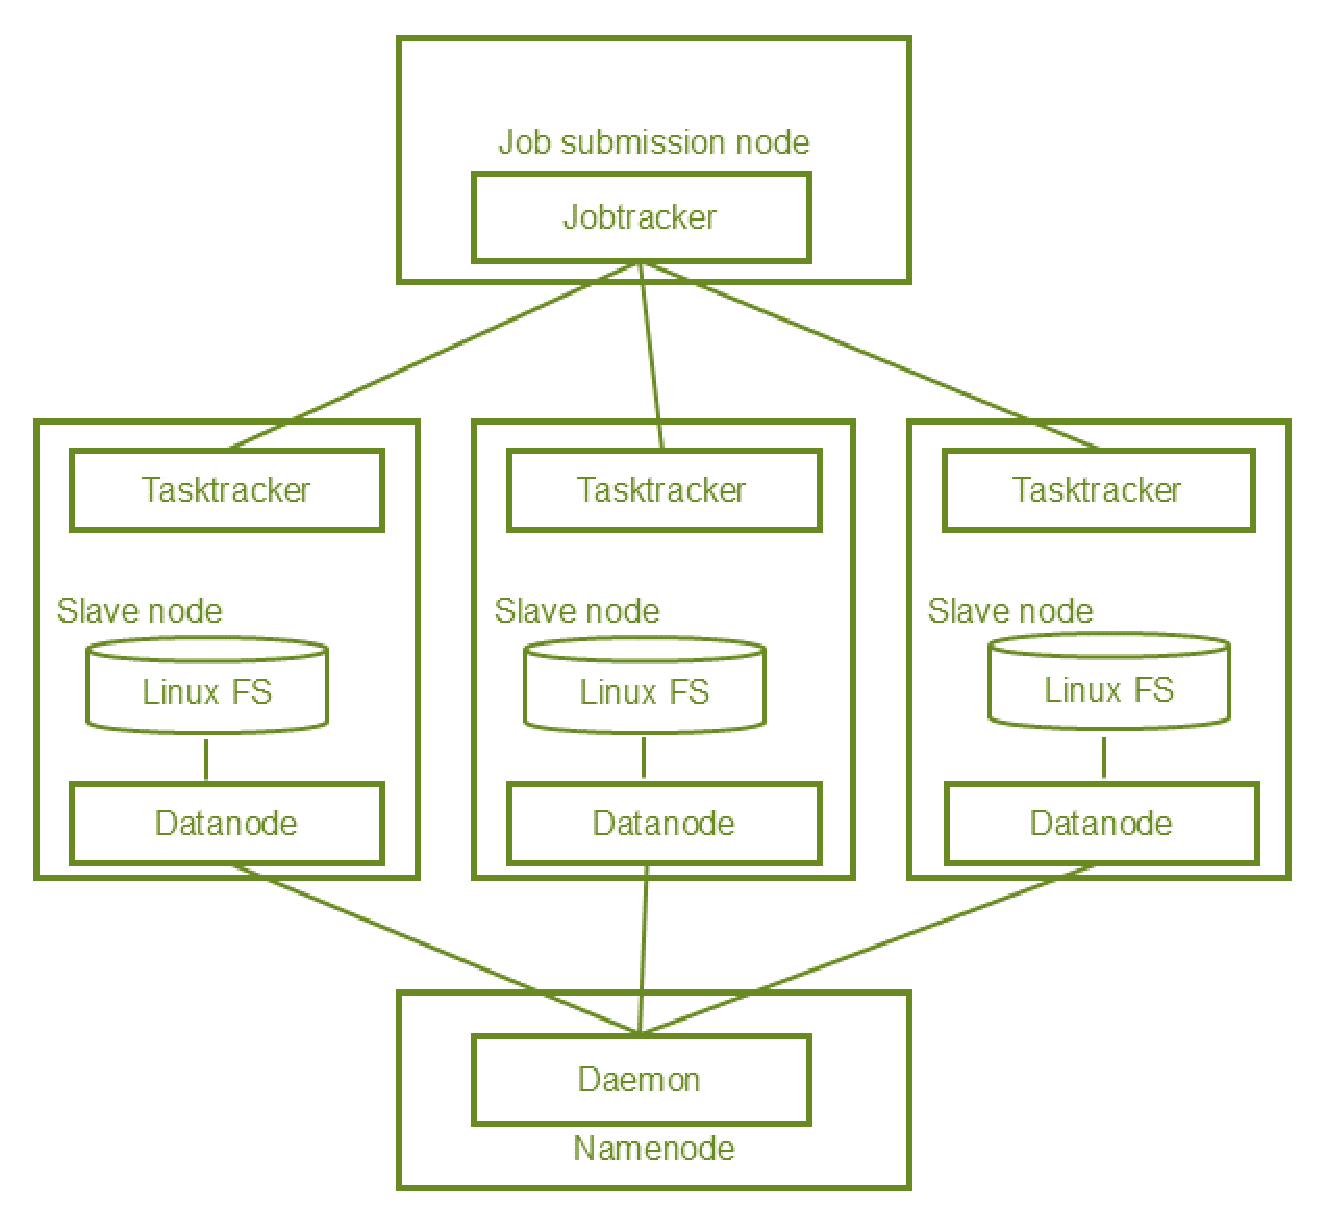
\includegraphics[width=1 \linewidth]{Thesis/Figures/Slide57.pdf}
\caption{\label{fig:hadoop}Node Work Flow in MapReduce Programming
Model \cite{ketu2020performance}}
\end{figure}

\subsection{Spark}

Apache Spark is a big data analytics framework based on distributed processing designed specifically for real-time data processing. Unlike Hadoop, which is based on disk-based computing, Spark uses in-memory computing, which significantly increases its processing speed. Spark supports multiple programming languages, including Python, Java and Scala and allows algorithms to be developed using any of these languages, unlike Hadoop, which relies on a single programming model. Spark also includes several specialised libraries, such as MLlib for machine learning, Spark SQL for structured data management and GraphX for graph processing. It supports parallel application development through Spark Streaming, which allows both real-time and batch data to be processed efficiently and quickly. \autoref{fig:spark} provides an overview of the Spark framework and its integration with higher-level tools and APIs. Core Spark is built on top of resilient distributed datasets \abk{RDD}{Resilient Distributed Datasets}, which can be sourced from internal storage such as HDFS, external storage, or created by other RDDs. These RDDs are managed using various storage options, including on-disk storage, in-memory serialised data and in-memory deserialised Java objects. \cite{ketu2020performance}

\begin{figure}[h]
\centering
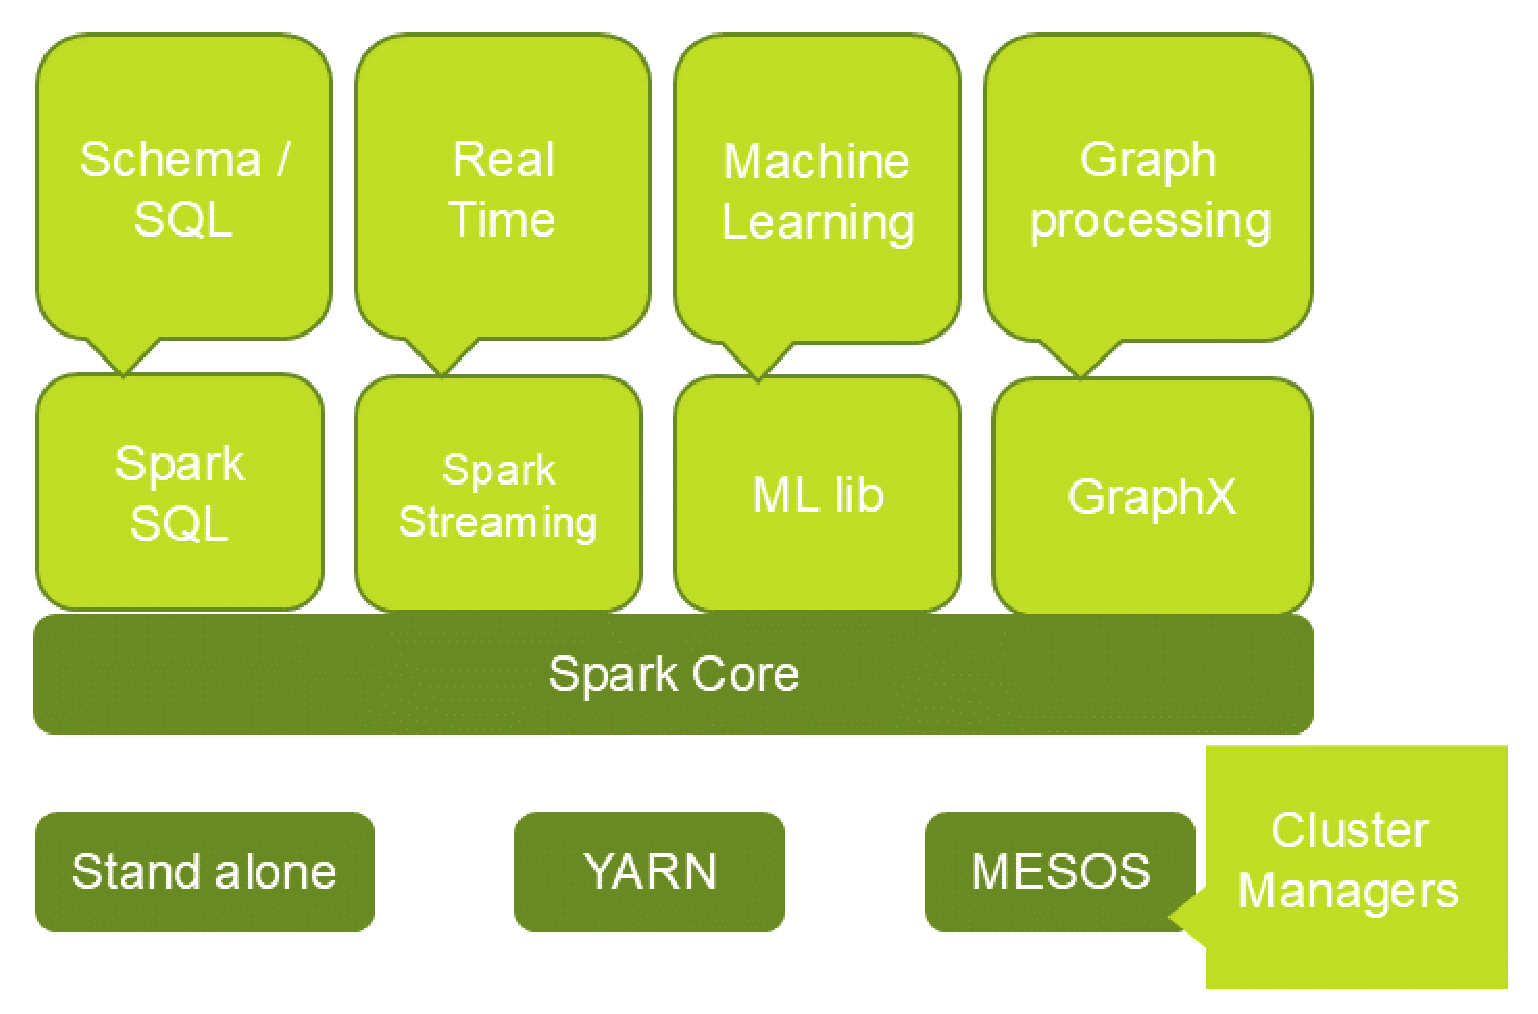
\includegraphics[width=0.8 \linewidth]{Thesis/Figures/Slide56.pdf}
\caption{\label{fig:spark}Spark Framework \cite{ketu2020performance}}
\end{figure}

Apache Spark provides stream processing capabilities through micro batching, where data streams are broken into small batches that are processed by Spark batch engine. While this approach is effective, it can still vary in performance compared to true stream processing frameworks. Spark is known for its unique features such as speed, ease of use, advanced analytics, in-memory computing and real time stream processing. It is exceptionally fast, up to 100 times faster than Hadoop and 10 times faster than disk based data access. It supports for multiple programming languages, making it easy for developers to use. Spark goes beyond basic map and reduce operations to support advanced analytics such as SQL queries, data streaming, machine learning and graph algorithms. It is highly flexible, running on different platforms such as Hadoop YARN, Mesos, EC2, Kubernetes, or as a standalone cluster in the cloud. Spark in-memory computing also enables iterative machine learning and complex data analysis at high speeds by keeping data in-memory. \cite{shaikh2019apache}

\subsection{Modin}

Modin is a framework designed to improve the performance of Pandas operations by enabling parallel execution with minimal changes to existing code bases. By simply modifying an import statement, users can take advantage of Modin optimizations to handle larger datasets more efficiently. The core of Modin architecture is to mimic the Pandas dataframe API while using parallel execution engines such as Ray or Dask as shown in \autoref{fig:modin}. \cite{shi2021leveraging}

\clearpage 

\begin{figure}[h]
\centering
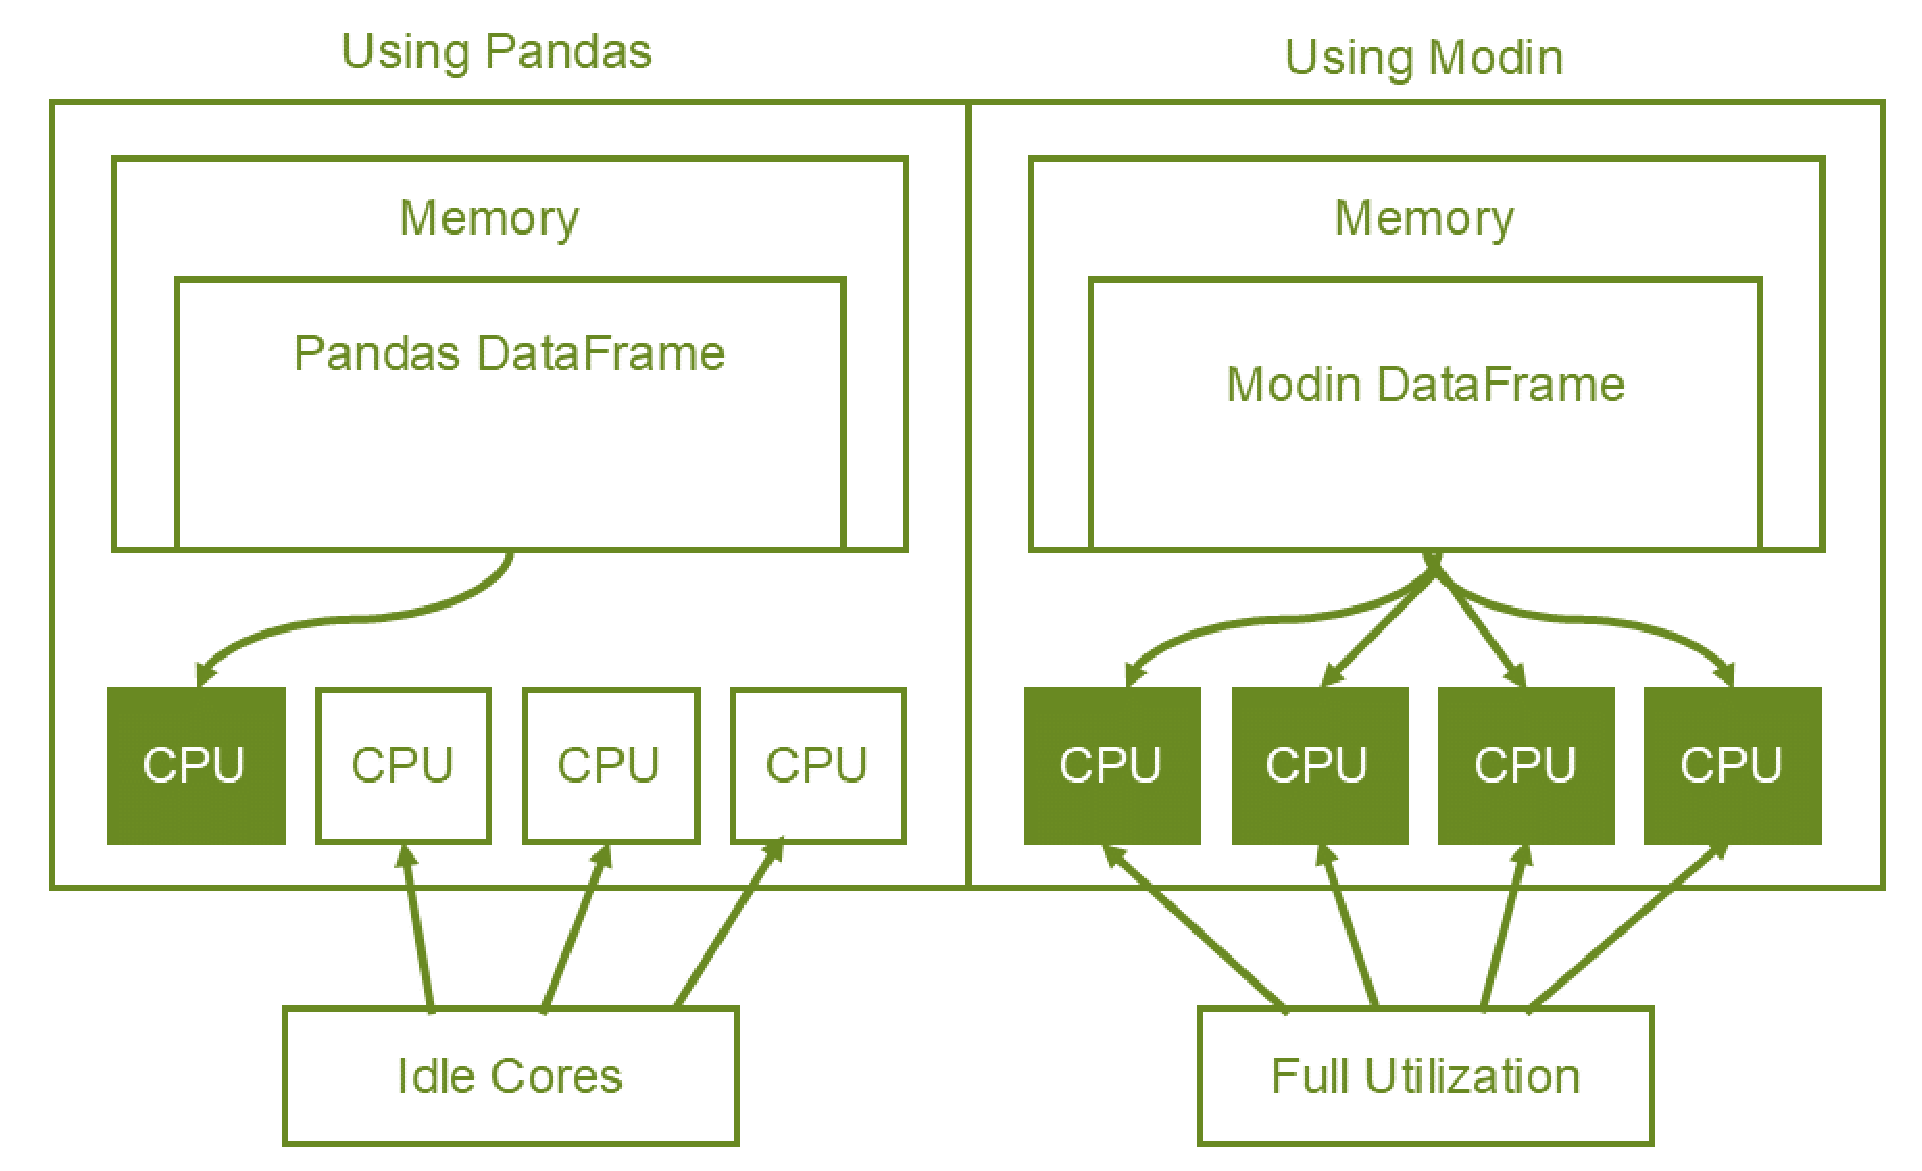
\includegraphics[width=1 \linewidth]{Thesis/Figures/Slide62.pdf}
\caption{\label{fig:modin}Modin Framework \cite{shi2021leveraging}}
\end{figure}



This allows Modin to translate high-level dataframe operations into a simplified set of basic algebraic operators such as select, join and map, making query planning and optimization easier. The traditional approach to Modin is eager execution, where queries are processed immediately as shown in \autoref{fig:eager modin}. \cite{shi2021leveraging}



\begin{figure}[h]
\centering
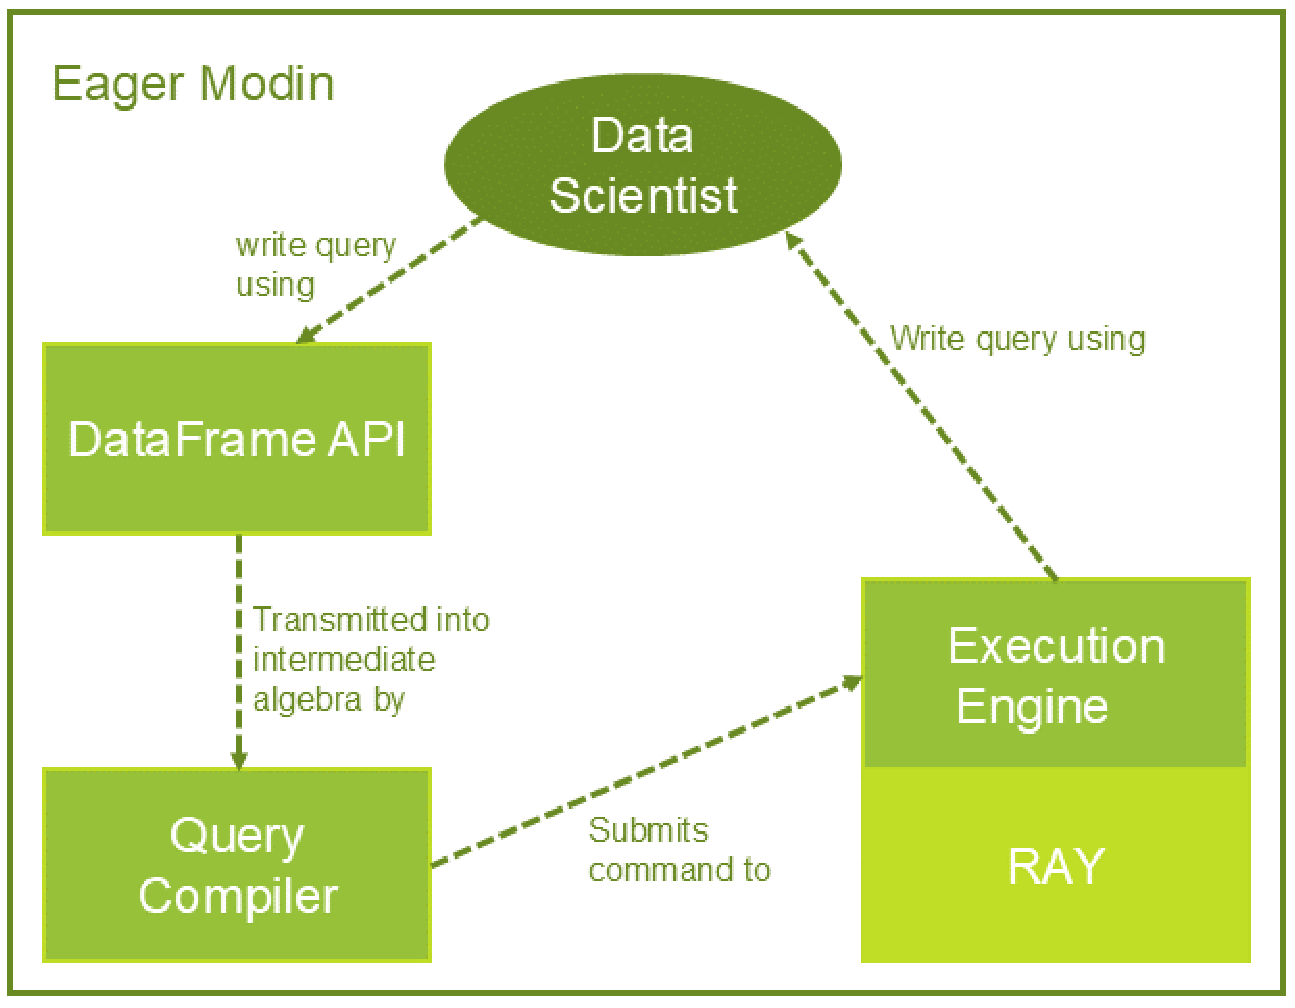
\includegraphics[width=0.8\linewidth]{Thesis/Figures/Slide64.pdf}
\caption{\label{fig:eager modin}Eager Modin Approach \cite{shi2021leveraging}}

\vspace{-20cm}
\end{figure}

\clearpage

However, New features of Modin include support for lazy execution, which delays query execution until explicitly requested by the user. This lazy approach allows optimization of query planning and collection of statistics during the users \texttt{think time} in interactive environments such as Jupyter notebooks, illustrated in \autoref{fig:lazy modin}. The underlying data in Modin dataframes is immutable and operations that appear destructive are implemented as copy on write, ensuring that the lazy execution framework handles updates efficiently. \cite{shi2021leveraging}



\begin{figure}[h]
\centering
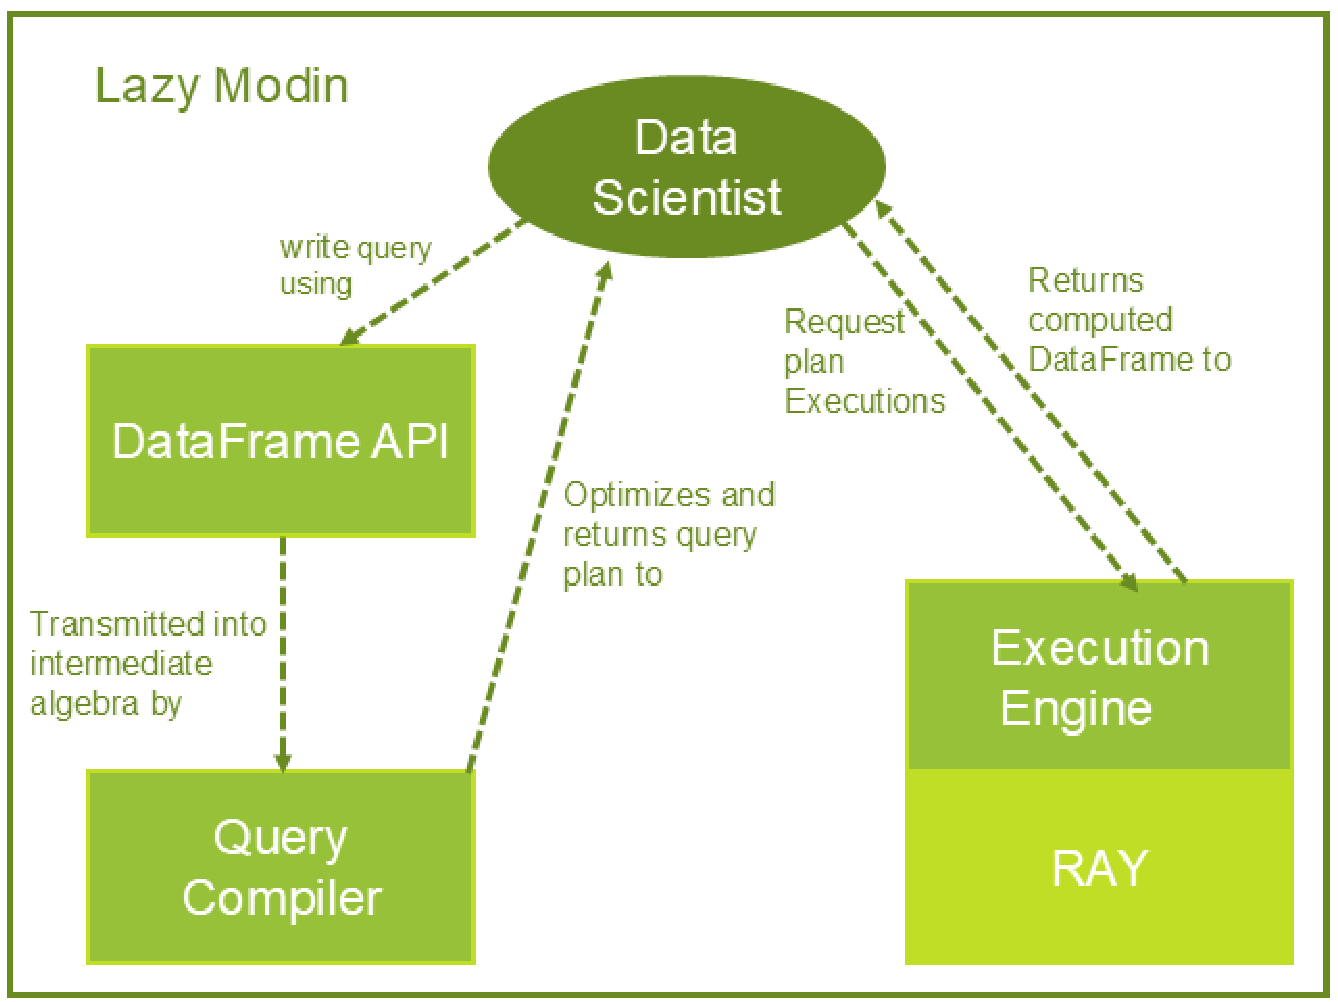
\includegraphics[width=0.8 \linewidth]{Thesis/Figures/Slide63.pdf}
\caption{\label{fig:lazy modin}Lazy Modin Approach \cite{shi2021leveraging}}
\end{figure}


\subsection{Dask}

Dask is a Python based big data engine that is gaining popularity for its ability to efficiently handle large-scale data processing tasks. Similar to Apache Spark, Dask uses in-memory computing, data locality and lazy evaluation to minimize unnecessary data transfers and computation. Dask workflows also take advantage of multithreading, allowing parallel processing when not constrained by Python global interpreter lock \abk{GIL}{Global Interpreter Lock}. Unlike Spark, which relies on coarse grained operations, Dask achieves fault tolerance through data lineage without this requirement, making it more flexible and modular. This modularity means that users can install only the components they need, keeping the system lightweight. Dask offers collection five main data structures tailored to different types of computation, Array, Bag, Dataframe, Delayed and Futures as shown in \autoref{fig:dask}. \cite{dugre2019performance}

\clearpage

\begin{figure}[h]
\centering
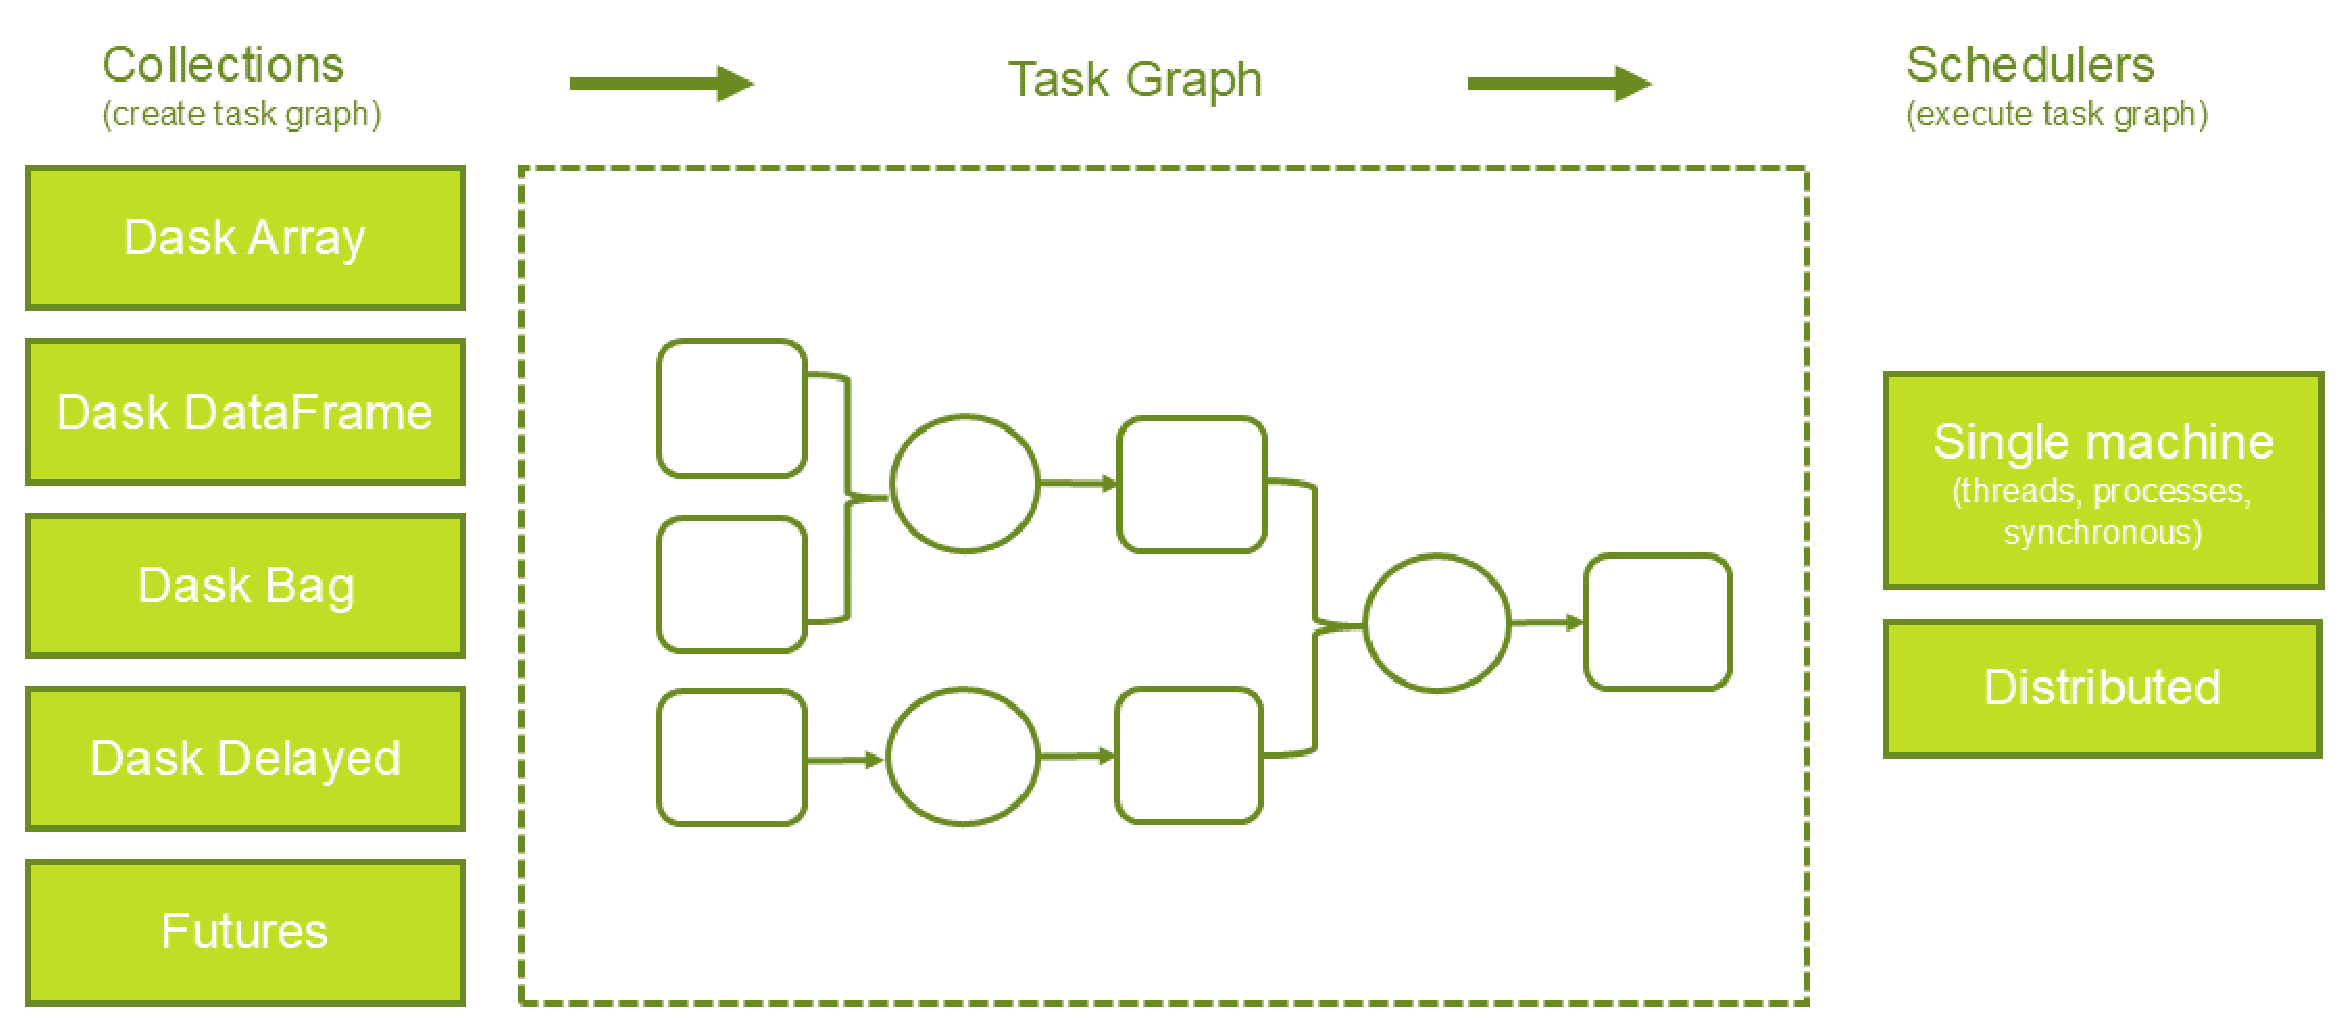
\includegraphics[width=1 \linewidth]{Thesis/Figures/Slide61.pdf}
\caption{\label{fig:dask}Dask Framework \cite{dask_docs}}
\end{figure}

Dask Array is designed for processing large numerical arrays and works as a distributed version of NumPy. Dask Bag, similar to Spark RDD, handles collections of Python objects and provides a parallel abstraction similar to the PyToolz library. The Dask dataframe allows parallel processing of large tabular datasets by distributing computations across multiple Pandas dataframes as shown in \autoref{fig:dask frame}. Dask Delayed is used to define custom tasks that don't fit into the other structures and supports lazy execution. In contrast, Dask Futures also handle arbitrary tasks, but operate in real time rather than waiting to be triggered. Most Dask structures use a local multi threaded scheduler by default, while Dask Bag specifically uses a multi processing scheduler. \cite{dugre2019performance}

\begin{figure}[h]
\centering
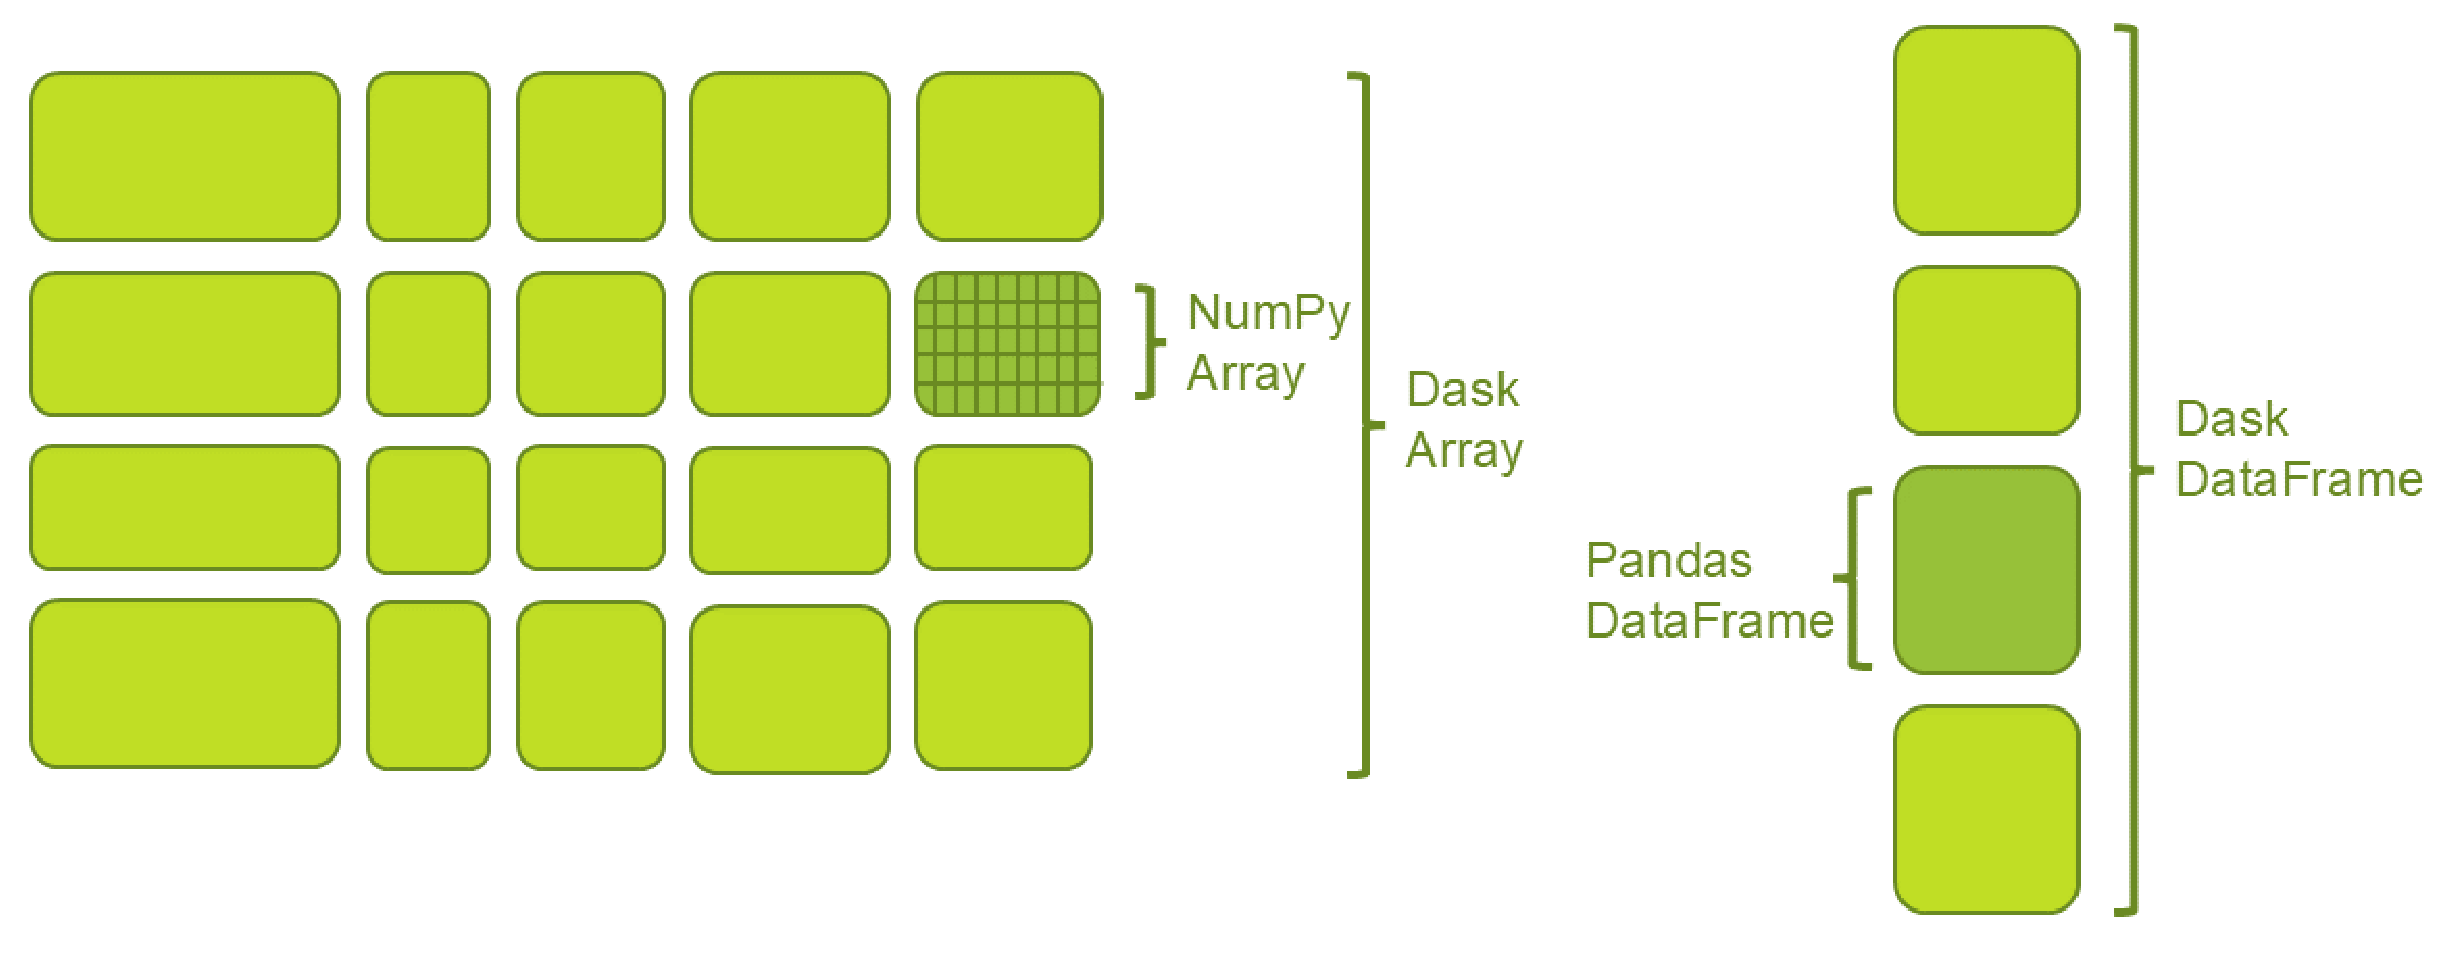
\includegraphics[width=1 \linewidth]{Thesis/Figures/Slide60.pdf}
\caption{\label{fig:dask frame}Dask Dataframe \cite{dask_docs}}
\end{figure}

\clearpage

\subsection{Optuna}

Optuna is an automated hyperparameter optimization framework designed specifically for machine learning. It offers a flexible API, define by run style, that enables user high modularity and dynamic construction of search spaces, thus providing a robust and adaptable solution for hyperparameter optimization of ML or DL models. Its lightweight, flexible and platform agnostic architecture enables the support of a wide range of tasks with minimal installation requirements. Optuna permits users to define search spaces in accordance with familiar Python syntax, including conditionals and loops. Furthermore, it employs algorithms to efficiently sample hyperparameters and prune unpromising trials and it facilitates straightforward parallelization, allowing studies to be scaled to encompass dozens or hundreds of workers with minimal code modifications as shown in \autoref{fig:optuna}. It also provides rapid visualization tools for the inspection of optimization histories through a variety of plotting functions. The framework is centered upon two principal concepts, first one is \texttt{study}, which represents an optimization based on an objective function and second is \texttt{trial}, which denotes a single execution of the objective function. \cite{optuna_docs}

\begin{figure}[h]
\centering
\includegraphics[width=1 \linewidth]{Thesis/Figures/Slide65.pdf}
\caption{\label{fig:optuna}Optuna Tuning Architecture \cite{optuna_hpo}}
\end{figure}

\subsection{TensorFlow}

TensorFlow is an open source library developed by Google for large-scale ML and DL tasks. It simplifies the development, training and optimization of machine learning models by combining computational algebra and optimization techniques. TensorFlow is highly efficient at performing complex mathematical calculations that are essential for ML and it uses tensors multi-dimensional arrays to encode data in ML or DL models. A key feature of TensorFlow is its ability to design data flow graphs, where data flows through a series of processing nodes, making it highly scalable and flexible across platforms such as cloud, mobile, desktop and web. TensorFlow provides two level of APIs low-level and high-level. Developer uses low-level APIs to build custom ML models and beginners uses high-level APIs which allows to interact with pre-built ML capabilities. TensorFlow architecture follows a simple three step process shown in \autoref{fig:TensorFlow}, the first being data preprocessing, which involves reading and transforming data for the model, then building the model and finally training, which uses optimization techniques such as back propagation to improve model accuracy and estimate model performance. TensorFlow serving is an important component of TensorFlow library, which is used to deploy ML models in production environment. It allows to have multiple versions of a model, which are called servables and can be deployed, updated and managed over a period of time. These servables can be created from lookup tables or complete models and can be deliver through streams of servable versions. The load of these servables is manged by TensorFlow source, to ensure smooth transitions between versions during serving. In addition, TensorFlow provides a highly, scalable and optimised environment developing, training and deploying ML models. \cite{ramchandani2022survey}

\begin{figure}[h]
\centering
\includegraphics[width=1 \linewidth]{Thesis/Figures/Slide66.pdf}
\caption{\label{fig:TensorFlow}TensorFlow Architecture \cite{ramchandani2022survey}}
\end{figure}

\subsection{Hyperopt}

Hyperopt is a library for optimising hyperparameters for algorithm configuration, especially in ML models. It handles complex search spaces that can include different types of variables such as continuous, ordinal and categorical, different sensitivity profiles such as uniform versus logarithmic scaling and conditional structures where different parameters become relevant depending on which classifier is chosen. As shown in \autoref{fig:Hyperopt}, the optimisation process involves several key steps. Data transformation is the first step, which prepares the raw data through preprocessing techniques such as normalisation or principal component analysis \abk{PCA}{Principal Component Analysis}. The second step is model selection, which involves choosing the appropriate ML models for the transformed data. The last step is hyperparameter optimisation. This involves defining a search domain where the hyperparameters are treated as random variables, specifying an objective function to evaluate model performance and using an optimisation algorithm (e.g. TPE) to explore the search space. Integration with scikit-learn facilitates model training and validation, while Hyperopt-sklearn extends these capabilities by handling complex pipelines of preprocessing steps and models. It also manages conditional hyperparameters and uses blacklist rules to ensure efficient and valid optimisation. \cite{komer2014hyperopt}


\begin{figure}[h]
\centering
\includegraphics[width=1 \linewidth]{Thesis/Figures/Slide67.pdf}
\caption{\label{fig:Hyperopt}Hyperopt Tuning \cite{hyperopt_bayesian_optimization}}
\end{figure}


\section{Comparison Criteria}

To evaluate Ray against other distributed computing tools such as Apache Spark, Dask, Modin, Optuna, Hyperopt and TensorFlow, several criteria are considered. These criteria focus on key aspects that influence the selection of a distributed computing framework based on specific use cases, including the following.

\begin{itemize}
    \item Scalability
    \item Performance
    \item Flexibility
    \item Cost
    \item Compatibility
    \item Ease of use
    
\end{itemize}

The ability of a distributed computation framework to be scaled up or down is a crucial criterion for selecting the appropriate framework, as it determines the systems ability to be economically deployed across a wide range of sizes and configurations. A scalable framework must achieve an effective balance between cost and performance, with effectiveness measured in terms of through-put and quality of service. The scalability of a system is measured by how well it performs across different sizes or levels, based on a specific metric that combines the original design and the scaling strategy. A good scaling strategy adjusts the system systematically as it grows, often using automated design optimization at each step. Efficient scaling shows how well the system is designed and helps identify areas for improvement, ensuring it can handle changing demands while maintaining good performance. Therefore, selecting a distributed computation framework with proven scalability ensures adaptability and performance across different operational scales. \cite{jogalekar2000evaluating}

Performance refers to the response time or throughput observed by the end user. It's common for distributed systems to not meet their performance goals when they are first built. Some systems work well with a small number of users, but lack the scalability to accommodate increased usage. Poor performance can lead to several negative outcomes, such as damaging customer relationships, reducing user productivity, losing revenue, increasing costs for fixing or redesigning the system and missing out on market opportunities in a timely manner. The majority of performance failures is due to lack of consideration on performance issues at an early stage of the development process, particularly within the architectural phase. It is therefore essential that a distributed computing framework is designed in a way that ensures the system's performance is consistently reliable, scalable and capable of meeting the demands of increasing workloads. It is of the utmost importance to consider performance issues at the architectural design phase, including factors such as synchronization mechanisms, resource allocation and load balancing. This will prevent future performance bottlenecks and ensure that the system can scale effectively as usage grows. \cite{smith2002performance}

The ability of distributed computing framework to adapt changing infrastructure is important factor in the selection of distributed computing framework. The flexibility of the infrastructure allows computing loads to be balanced on the fly as more users join the system. The process of setting up the infrastructure has become so standardised that adding computing resources has become almost as simple as adding building blocks to an existing grid. Flexibility in distributed computing framework is also important because, it helps to manage the different workloads efficiently. As the number of user increases, the system can more effectively balance the demand, making it easier to manage, while also benefiting from cost savings as it grows. Therefore, flexibility is essential to consider in order to achieve the distributed system that can dynamically adjust to changing demands while maintaining performance and avail benefits of scalability and resource optimization. \cite{avram2014advantages}

The cost of distributed computing framework considered as a significant criteria in selection of distributed computing framework, as it allow to execute large and complex processing task with minimum resources which make it accessible for smaller companies, which used to be available only to large organizations. This makes it a good choice for organizations looking to save cost both in terms of financially and computing resources. Furthermore, cloud computing frameworks enables the dynamic allocation of resources, which is beneficial for computational tasks that require computing power for relatively short periods of time. Affordability and scalability of resources makes cost a key factor in choosing a distributed computing framework for organization. \cite{avram2014advantages}

When selecting a distributed computing framework, compatibility is the important criteria, as it guarantees the easy of integration with current tools and technologies. Distributed systems is based on combination of different independent components or services. To work effectively with each other compatibility between components or resources is essential. The interaction protocols are used to determine how these components can communicate with each other and have a significant impact on their compatibility. The ability of a framework to follow these communication protocols and to integrate with different components or services reduces the need for extensive modifications and helps to avoid potential integration problems. Compatibility therefore not only simplifies implementation, but also increases the overall flexibility and scalability of distributed computing systems. \cite{chevrou2019modular}

When choosing a distributed computing framework, it is essential to prioritize ease of use. As this has a direct impact on developer productivity and efficiency. An easy to use framework simplifies the development process by providing intuitive APIs and clear abstractions. Allowing developers to focus on solving domain specific problems rather than managing complex distributed systems. The frameworks with well designed interfaces and extensive documentation reduce the time required to learn and deploy applications effectively. Prioritizing usability in the selection process ensures that distributed computing can be used effectively, maximizing both developer satisfaction and project success. \cite{zaharia2012resilient}.



\section{Comparison of Ray Core with Apache Spark and Dask}


The Ray core is discussed earlier in this report and provides primitive methods such as tasks, actors and objects that are used to develop scalable and distributed computing resources \cite{ray_doc}. \autoref{tab:table1} present a comparison of Ray core with Apache Spark and Dask, focusing on how these frameworks manage distributed computing tasks. The evaluation is based on criteria such as scalability, performance, flexibility, cost, compatibility and ease of use, which are essentials factors in distributed computing, particularly in the context of large-scale applications or big data processing.


\begin{table}[h]
\centering

\begin{tabular}{|p{2.6cm}|p{4cm}|p{4cm}|p{4cm}|}
\hline
\textbf{Feature} & \textbf{Ray Core} & \textbf{Apache Spark} & \textbf{Dask} \\
\hline
\textbf{Scalability} & Provide high scalability, can scale across many node and cores. \cite{ray_doc} & Provide high scalability for large-scale data. \cite{apache_spark}& Ability to scale is limited for large dataset \cite{dask_docs} \\
\hline
\textbf{Performance} & High performance with low overhead, efficient for distributed tasks. \cite{ray_doc} & High performance, due to in-memory processing but have higher latency due to disk based storage \cite{apache_spark}&Good performance, for Python based tasks, but need tuning for large-scale use. \cite{dask_docs} \\
\hline
\textbf{Flexibility} & supports various distributed computing paradigms including task and actor models. \cite{ray_doc}& Flexible with rich APIs, supports many data formats. \cite{apache_spark}& Modular design allow users to install only the required components. \cite{dugre2019performance}\\
\hline
\textbf{Cost} & Cost effective, require dedicated resources for monitoring, scaling and handling failures. \cite{ray_doc} & Operational cost overhead including monitoring, scaling and handling failures. \cite{apache_spark}& Cluster involves operational overhead, including monitoring and optimizing performance. \cite{dask_docs}\\
\hline
\textbf{Compatibility} & Support Python and integration with other Ray libraries for diverse workflows. \cite{ray_doc} & Support Python, R and Scala \cite{apache_spark}& Integrate easily with Python libraries and workflows. \cite{dask_docs} \\
\hline
\textbf{Ease of Use} & Easy to use for Python developers, very well documented. & Multi language support make it suitable for majority of developers. & User friendly for Python developer\\
\hline
\end{tabular}
\caption{Comparison of Ray Core, Apache Spark and Dask Features}
\label{tab:table1}
\end{table}

\section{Comparison of Ray Data with Apache Spark and Modin}


Ray Data was discussed in the previous chapter as a tool that facilitates distributed data processing and integrates seamlessly into ML workloads \cite{ray_doc}. In this section, Ray Data is compared to other popular distributed data processing tools to assess its strengths and weaknesses. The \autoref{tab:table2} provides a comparative analysis of Ray Data, Apache Spark and Modin across several important dimensions like scalability, performance, flexibility, cost, compatibility and ease of use. In context of Ml workloads, scaling APIs and Data Processing.

\begin{table}[ht]
\centering
\begin{tabular}{|p{3cm}|p{3.5cm}|p{3.5cm}|p{3.5cm}|}
\hline
\textbf{Feature} & \textbf{Ray Data} & \textbf{Apache Spark} & \textbf{Modin} \\
\hline
\textbf{Scalability} & Highly scalable for distributed workloads with dynamic task distribution across nodes. \cite{ray_doc}& Highly scalable and optimized for batch processing. \cite{apache_spark} & Provide scalability with Ray backend, suitable for dataframe operations. \cite{modin_docs} \\
\hline
\textbf{Performance} & Suitable for both small and large-scale data processing. \cite{ray_doc} & High performance, optimize memory usage can avoid memory errors. \cite{apache_spark}& High performance for large dataset, which even cannot fit in-memory. \cite{modin_docs}\\
\hline
\textbf{Flexibility} & Very flexible, supports various task, actor and models. \cite{ray_doc}& Vast ecosystem have many data processing option. \cite{apache_spark} &Flexible approach in dataframe operation. \cite{modin_docs} \\
\hline
\textbf{Cost} & Fast and cheap for ML applications. \cite{ray_doc}& Can be costly when scaling resources. \cite{apache_spark}& Cost effective but scales with the size of the data and operation. \cite{modin_docs} \\
\hline
\textbf{Compatibility} & Integrates well with TensorFlow, PyTorch and other libraries. \cite{ray_doc}& Broad compatibility with data formats and resources. \cite{apache_spark} & Compatible with Pandas and Python tools. \cite{modin_docs} \\
\hline
\textbf{Ease of Use} & Easy to use for Python developers, very well documented. & Require knowledge of Spark APIs. \cite{apache_spark}& Easy to use Pandas like APIs. \cite{modin_docs} \\
\hline
\end{tabular}
\caption{Comparison of Ray Data, Apache Spark and Modin Features}
\label{tab:table2}
\end{table}

\clearpage

\section{Comparison of Ray Train with Apache Spark and Dask}


Ray Train is a distributed training library within the Ray ecosystem designed to facilitate large-scale ML models by enabling efficient training across multiple GPUs or nodes. In this section, Ray train in is evaluated against Apache Spark and Dask, highlighting its strengths and weaknesses relative to these popular distributed computing frameworks. \autoref{tab:table3} provides a comparative analysis across several important dimensions like scalability, performance, flexibility, cost, compatibility and ease of use. These criteria are critical when evaluating tools for scaling and distributed training. \cite{ray_doc}

\begin{table}[ht]
\centering
\begin{tabular}{|p{2.5cm}|p{3.8cm}|p{3.3cm}|p{3.8cm}|}
\hline
\textbf{Feature} & \textbf{Ray Train} & \textbf{Apache Spark} & \textbf{Dask} \\
\hline
\textbf{Scalability} & Highly scalable ML libraries for distributed training. \cite{ray_doc} & Offer manual optimization of memory caching, which provide high scalability while training. \cite{garcia2017comparison}& Provide Dask cluster to parallelize workload on many machines to train ML models. \cite{dask_docs}\\
\hline
\textbf{Performance} & High performance for distributed training tasks and workflows. \cite{ray_doc} & Provide iterative computation, enabling MLlib to run fast \cite{apache_spark} & Provide Dask scheduler to understand the characteristics of computations. \cite{dask_docs}\\
\hline
\textbf{Flexibility} & Provide support for frameworks like PyTorch, TensorFlow, XGBoost and many others. \cite{ray_doc} & Provide interoperating with libraries like NumPy and R. \cite{apache_spark} & Allows to deploys XGBoost alongside Dask. \cite{dask_docs}\\
\hline
\textbf{Cost} & Cost effective due to dynamic scaling using actors. \cite{ray_doc}& Perform fast distributed computing using in-memory primitives. \cite{garcia2017comparison} & Not able to cope with datasets larger then machine memory. \cite{dask_docs} \\
\hline
\textbf{Compatibility} & Provide ecosystem of API to interact with different training framework. \cite{ray_doc} & Compatible with Kubernetes, Hadoop, Apache Mesos, standalone, or in the cloud. \cite{apache_spark}& Compatible with Scikit-learn library for distributed training. \cite{dask_docs}\\
\hline
\textbf{Ease of Use} & Easy to use for Python developers, very well documented. & Require knowledge of NumPy, R and Spark APIs. \cite{apache_spark}& Easy to use for Python developers. \\
\hline

\hline
\end{tabular}
\caption{Comparison of Ray Train, Apache Spark and Dask Features}
\label{tab:table3}
\end{table}


\clearpage

\section{Comparison of Ray Tune with Optuna and Hyperopt}


Ray Tune is an advanced library within the Ray ecosystem that specializes in hyperparameter optimization for machine learning models. It uses Ray infrastructure to manage and execute tuning tasks across multiple nodes. Ray Tune supports a wide range of optimization algorithms and integrates seamlessly with ML frameworks, making it suitable for complex and large-scale tuning tasks. \autoref{tab:table4}, provide a comparison of Ray Tune with other popular tuning libraries to identify its benefits. \cite{ray_doc}



\begin{table}[ht]
\centering
\begin{tabular}{|p{3cm}|p{3.8cm}|p{3.8cm}|p{3.8cm}|}
\hline
\textbf{Feature} & \textbf{Ray Tune} & \textbf{Optuna} & \textbf{	Hyperopt} \\
\hline
\textbf{Scalability} & Allows transparently parallelize across multiple GPUs and multiple nodes. \cite{ray_doc}& Provide easy parallelization with little or no change to code. \cite{optuna_docs} & Allowing massive scale-out for tuning using \texttt{SparkTrials}. \cite{hyperopt_docs}\\
\hline
\textbf{Performance} & Can change hyperparameters during training to optimize schedules. \cite{ray_doc}& Enable optimize hyperparameter tuning by pruning unpromising trials. \cite{optuna_docs} & Optimize tuning by using normalization and PCA methods. \cite{komer2014hyperopt}\\
\hline
\textbf{Flexibility} & Allow to integrate variety of popular tuning libraries to scale up optimization process. \cite{ray_doc}& Provide \texttt{Ask-and-Tell} interface for flexibility in hyperparameter optimization. \cite{optuna_docs}& Provide flexibility to specifying an objective function to minimize. \cite{hyperopt_docs} \\
\hline
\textbf{Cost} & Reduce cost of tuning by terminating bad runs early. \cite{ray_doc} & High computation cost in categorical and conditional hyperparameters tuning. \cite{optuna_docs} & Use early stop feature which help in using less computational resources. \cite{pokhrel2023comparison}\\
\hline
\textbf{Compatibility} & Integrates with wide range of hyperparameter optimization tools. \cite{ray_doc} & Provide versatile and platform agnostic architecture. \cite{optuna_docs} & Integrates well with ML libraries like scikit-learn and TensorFlow. \cite{hyperopt_docs} \\
\hline
\textbf{Ease of Use} & Easy to setup and experiment with different algorithms. \cite{ray_doc} & Similar to Python syntax including conditionals and loops. \cite{optuna_docs}& Defining search space and objective function require in depth knowledge. \cite{hyperopt_docs}\\
\hline

\hline
\end{tabular}
\caption{Comparison of Ray Tune, Optuna and Hyperopt Features}
\label{tab:table4}
\end{table}

\clearpage

\section{Comparison of Ray Serve with TensorFlow Serve}


Ray Serve is a scalable model serving library for building online inference APIs. It is especially effective for model composition and serving numerous models, allowing you to create complex inference services that integrate multiple ML models along with business logic. \autoref{tab:table5}, shows a comparison of Ray serve with TensorFlow serving library highlighting there features and capabilities. \cite{ray_doc}


\begin{table}[ht]
\centering
\begin{tabular}{|p{3cm}|p{5cm}|p{6cm}|}
\hline
\textbf{Feature} & \textbf{Ray Serve} & \textbf{TensorFlow Serving} \\
\hline
\textbf{Scalability} & Easy to scale and provide scheduling support. \cite{ray_doc} & The size and scale of serving TensorFlow model is flexible, but provide single model architectures. \cite{tensorflow} \\
\hline
\textbf{Performance} & Use response streaming, dynamic request batching, multi-node/multi-GPU serving for performance Optimization. \cite{ray_doc} & High performance for TensorFlow models with batching and GPU support optimizations. \cite{tensorflow}\\
\hline
\textbf{Flexibility} & Ray Serve is framework agnostic, so you can use a single toolkit to serve everything. \cite{ray_doc} & Allow TensorFlow model serving can be of any type and interface, also future improvements like streaming results, experimental APIs and asynchronous modes of operation are possible. \cite{tensorflow} \\
\hline
\textbf{Cost} & Dynamically scale up and down resources to save cost \cite{ray_doc} & Cost-efficient for TensorFlow model but serving for non-TensorFlow model can increase cost and complexity. \cite{tensorflow}\\
\hline
\textbf{Compatibility} & Allow to combine multiple ML models, business logic and expressive HTTP handling. \cite{ray_doc} & Highly compatible with TensorFlow model, For non-TensorFlow model need to analyze model structure and apply optimization to make it compatible. \cite{tensorflow} \\
\hline
\textbf{Ease of Use} & Easy to use for Python developers, very well documented. & Well documented and designed for TensorFlow practitioners, although it offers little flexibility in terms of connecting with non-TensorFlow tools. \cite{tensorflow} \\
\hline

\hline
\end{tabular}
\caption{Comparison of Ray Serve and TensorFlow Serve Features}
\label{tab:table5}
\end{table}

\clearpage


\section{Discussion on Comparison of Distributed Computing Tools}

In comparing and exploring different distributed computing tools, Ray stands out as an efficient framework that provides seamless integration across different phases of a data-driven pipeline, including model training, hyperparameter optimization and model serving. Dask is the fastest framework, but is less scalable compared to Ray and Spark. Spark's performance is intermediate between Ray and Dask and improves as the number of nodes increases. For read-intensive applications, Dask is a good choice when only a few nodes are available, while Spark or Ray are recommended for larger numbers of workers. Modin provides Pandas APIs for distributed computing, but Ray Data goes beyond Modin to provide advanced in-memory distributed computing capabilities \cite{modin_docs}. For hyperparameter optimization, Optuna and Hyperopt are powerful tools but lack the scalability of Ray Tune. For end to end pipeline integration, Ray Serve is deeply integrated with other Ray libraries, enabling seamless model deployment. In contrast, TensorFlow Serving is more standalone and specialised, making integration in multi-framework environments more challenging \cite{tensorflow}. To draw further conclusions, it is highly recommended to implement these advanced frameworks and analyse their performance across different tasks such as data pre-processing, model training, hyperparameter optimization and model serving. \cite{baglioni2023large}




            
            \chapter{Conclusion and Outlook}

This thesis explains the implementation of a cloud-native architecture designed for secure, scalable, and distributed computing, with a focus on authentication, authorization, and the deployment of AI models. The primary objective is to address the challenges posed by modern cloud-native environments, particularly in ensuring security, scalability, and the efficient management of distributed workloads. The first major component of this research was to integrate an authentication module using Keycloak with ArgoCD to ensure that only authorized users can access and manage application deployments. Keycloak was chosen because of IAM capabilities that offer SSO and include support of various authentication schemes such as OAuth and OIDC \cite{keycloak_doc}. This approach provide ArgoCD a secure access point and helps in centralizing and streamlining user administration \cite{keycloak_doc}. The second part of the research is to implement authorization using Kubernetes RBAC, to manage fine-grained access control, and make sure that users and services only had the necessary permissions to interact with resources in the cluster \cite{Kubernetes_doc}. The principle of least privilege was implemented by using Kubernetes RBAC in combination with roles, role bindings, cluster roles, and cluster role bindings, which improve the security of the cluster and reduced the potential risk in the cloud-native environment \cite{Kubernetes_doc}. Thus, by automating the process of creating users and assigning roles using RBAC configurations, we can efficiently manage roles and access policies across the cluster \cite{Kubernetes_doc}. The third of this research was the implementation of scalable and distributed architecture for AI models using the Ray framework. Ray is a complete ecosystem for data processing, training , tuning, serving and processing of large-scale AI workloads by enabling autoscaling through Kubernetes HPA \cite{ray_doc}. Integrating KubeRay with the Kubernetes cluster ensured that resources can be dynamically scale based on the computational demand, optimizing the use of both CPU and GPU resources \cite{ray_doc}. This enables to process large datasets and complex AI models in a cloud-native environment with high flexibility and performance \cite{ray_doc}. By addressing critical issues of authentication, authorization, and resource distribution, this report illustrate how cloud-native architectures can be used to achieve security, scalability, and effectively handle distributed workloads. Utilizing tools like Keycloak, Kubernetes RBAC, and Ray helps to address typical issues in cloud-native environments, making the architecture well suited for modern AI-driven applications.

In the future, frameworks such as Apache Spark, Dask, Modin, Optuna, Hyperopt, and TensorFlow Serve will be implemented and compared in order to investigate distributed computing options outside of Ray. The evaluation of these frameworks in this research has been primarily based on documentation; however, the next step will be to use these frameworks to implement cloud-native architectures. This experimentation will allow a thorough comparison of their performance in terms of scalability, resource efficiency, ease of integration and overall system responsiveness. Comparing these frameworks with Ray for large datasets and using advanced libraries to train ML and DL models will provide valuable insights into bottlenecks, strengths and weaknesses in managing distributed AI workloads. This future research will provide a more comprehensive understanding of these tools and help to further optimise the deployment of scalable AI models in cloud-native architectures.

		% Folgender Befehl erzwingt an entsprechender Stelle einen Seitenumbruch
		% Bei einer Seite bitte ausblenden
%		\addtocontents{toc}{\protect\newpage}
	%%%%%%%%%%%%%%%%%%%%%%%%%%%%%%%%%%%%%%%%%%%%%%%%%%%%%%%%%%%%%%%%%%%%%%%%%%%%%%%%%%%%%%%%%%%%%%
	%%%%   DO NOT CHANGE                                                                       %%%
	%%%%%%%%%%%%%%%%%%%%%%%%%%%%%%%%%%%%%%%%%%%%%%%%%%%%%%%%%%%%%%%%%%%%%%%%%%%%%%%%%%%%%%%%%%%%%%
	
	\cleardoublepage
\thispagestyle{plain}

% Inhaltsverzeichnis-Eintrag
\titlecontents{chapter}
[0em]
{\vspace{12pt}}
{\contentslabel{1em}}
{}
{\vzPunkte\contentspage}

% Code für Linksbuendigkeit der Klammern 
\makeatletter 
	\renewcommand*{\@biblabel}[1]{\makebox[\labelwidth][l]{[#1]}}
\makeatother

% Label-Width - Eintrag entspricht max. Anzahl an Ziffern
\setbiblabelwidth{99}

% Literaturverzeichnis Stil
% 2023/06/23: changes bibliography style to a English one
\bibliographystyle{ieeetr}
%	Pfad:		C:\Program Files (x86)\MiKTeX 2.9\miktex\bin\bibtex.exe
%	Argumente:	"%bm"}
% Am besten aus Citavi exportieren
\bibliography{Verzeichnis_Literatur}


%%%%%% Extra Verzeichnisse %%%%%
\cleardoublepage
\thispagestyle{plain}

% Inhaltsverzeichnis-Eintrag
\titlecontents{chapter}
[0em]
{}
{\contentslabel{1em}}
{}
{\vzPunkte\contentspage}

%%%%% Quellenverzeichnis %%%%%%

% Label-Width - Eintrag entspricht max. Anzahl an Ziffern
\setbiblabelwidth{9}


%	Postprozessor:
		%Anwendung: 	bibtex.exe
		%Argumente:		Q



%% Layout Inhaltsverzeichnis wiederherstellen
%\input{Format_ToC}	% Literaturverzeichnis (BibTeX)	
	
	\appendix										% Beginn des Anhangs
	% Bezeichnungen und Nummerierungsstile
\renewcommand{\chaptername}{Anhang}
% \renewcommand{\theequation}{\Alph{section}.\arabic{equation}}
\renewcommand{\theequation}{\Alph{chapter}.\arabic{equation}}
\renewcommand{\thetable}{\Alph{chapter}.\arabic{table}}
\renewcommand{\thefigure}{\Alph{chapter}.\arabic{figure}}


% Inhaltsverzeichnislayout fuer 'Anhang'
\titlecontents{chapter}
[1em]	% Abstand linker Textrand bis Kapitelueberschriften
{}	% Textformatierung
{\contentslabel{1em}}	% Abstand und Nummerierung vor Kapitelueberschriften
{}
{\vzPunkte\contentspage} % Formatierung nach Titel bis zur Seitenzahl


% Erscheinen von 'Anhang' im Inhaltsverzeichnis
%\addtocontents{toc}{\protect\contentsline{chapter}{Anhang}{}{}}

				% Formatierung des Anhangs
		%
	%%%%%%%%%%%%%%%%%%%%%%%%%%%%%%%%%%%%%%%%%%%%%%%%%%%%%%%%%%%%%%%%%%%%%%%%%%%%%%%%%%%%%%%%%%%%%%
	%%%%   FILL WITH OWN CONTENT, IF APPLICABLE                                                %%%
	%%%%%%%%%%%%%%%%%%%%%%%%%%%%%%%%%%%%%%%%%%%%%%%%%%%%%%%%%%%%%%%%%%%%%%%%%%%%%%%%%%%%%%%%%%%%%%

%
%	The insertion of attachments is done here:
%

		%\chapter{Appendix}
\label{A_Appendix}
% 
Hier kommt das hin, was in der Ausführung für Unübersichtlichkeit gesorgt
hätte...

		
		%\includepdf[pages=1-2, scale=0.75, pagecommand={\thispagestyle{fancy}}, offset=0.5cm 1.5cm]{Test_Anhang.pdf}
		%\cleardoublepage
		
		
	%%%%%%%%%%%%%%%%%%%%%%%%%%%%%%%%%%%%%%%%%%%%%%%%%%%%%%%%%%%%%%%%%%%%%%%%%%%%%%%%%%%%%%%%%%%%%%
	%%%%  CV IF DESIRED (adjust the command \Lebenslauf above accordingly)                     %%%
	%%%%%%%%%%%%%%%%%%%%%%%%%%%%%%%%%%%%%%%%%%%%%%%%%%%%%%%%%%%%%%%%%%%%%%%%%%%%%%%%%%%%%%%%%%%%%%
	
	\ifthenelse{\equal{\Lebenslauf}{CV}}{
		\currentpdfbookmark{Curriculum Vitae}{Curriculum Vitae}	% Lesezeichen fuer Lebenslauf
		\thispagestyle{empty}
		\includepdf[pages={1},offset= {0.5cm, -0.5cm}]{CV/CurriculumVitae.pdf}
		\cleardoublepage
	}{}
 
\end{document}

